%% bare_jrnl.tex
%% V1.3
%% 2007/01/11
%% by Michael Shell
%% see http://www.michaelshell.org/
%% for current contact information.
%%
%% This is a skeleton file demonstrating the use of IEEEtran.cls
%% (requires IEEEtran.cls version 1.7 or later) with an IEEE journal paper.
%%
%% Support sites:
%% http://www.michaelshell.org/tex/ieeetran/
%% http://www.ctan.org/tex-archive/macros/latex/contrib/IEEEtran/
%% and
%% http://www.ieee.org/



% *** Authors should verify (and, if needed, correct) their LaTeX system  ***
% *** with the testflow diagnostic prior to trusting their LaTeX platform ***
% *** with production work. IEEE's font choices can trigger bugs that do  ***
% *** not appear when using other class files.                            ***
% The testflow support page is at:
% http://www.michaelshell.org/tex/testflow/


%%*************************************************************************
%% Legal Notice:
%% This code is offered as-is without any warranty either expressed or
%% implied; without even the implied warranty of MERCHANTABILITY or
%% FITNESS FOR A PARTICULAR PURPOSE! 
%% User assumes all risk.
%% In no event shall IEEE or any contributor to this code be liable for
%% any damages or losses, including, but not limited to, incidental,
%% consequential, or any other damages, resulting from the use or misuse
%% of any information contained here.
%%
%% All comments are the opinions of their respective authors and are not
%% necessarily endorsed by the IEEE.
%%
%% This work is distributed under the LaTeX Project Public License (LPPL)
%% ( http://www.latex-project.org/ ) version 1.3, and may be freely used,
%% distributed and modified. A copy of the LPPL, version 1.3, is included
%% in the base LaTeX documentation of all distributions of LaTeX released
%% 2003/12/01 or later.
%% Retain all contribution notices and credits.
%% ** Modified files should be clearly indicated as such, including  **
%% ** renaming them and changing author support contact information. **
%%
%% File list of work: IEEEtran.cls, IEEEtran_HOWTO.pdf, bare_adv.tex,
%%                    bare_conf.tex, bare_jrnl.tex, bare_jrnl_compsoc.tex
%%*************************************************************************

% Note that the a4paper option is mainly intended so that authors in
% countries using A4 can easily print to A4 and see how their papers will
% look in print - the typesetting of the document will not typically be
% affected with changes in paper size (but the bottom and side margins will).
% Use the testflow package mentioned above to verify correct handling of
% both paper sizes by the user's LaTeX system.
%
% Also note that the "draftcls" or "draftclsnofoot", not "draft", option
% should be used if it is desired that the figures are to be displayed in
% draft mode.
%
\documentclass[journal,twocolumn]{IEEEtran}
%
% If IEEEtran.cls has not been installed into the LaTeX system files,
% manually specify the path to it like:
% \documentclass[journal]{../sty/IEEEtran}





% Some very useful LaTeX packages include:
% (uncomment the ones you want to load)


% *** MISC UTILITY PACKAGES ***
%
%\usepackage{ifpdf}
% Heiko Oberdiek's ifpdf.sty is very useful if you need conditional
% compilation based on whether the output is pdf or dvi.
% usage:
% \ifpdf
%   % pdf code
% \else
%   % dvi code
% \fi
% The latest version of ifpdf.sty can be obtained from:
% http://www.ctan.org/tex-archive/macros/latex/contrib/oberdiek/
% Also, note that IEEEtran.cls V1.7 and later provides a builtin
% \ifCLASSINFOpdf conditional that works the same way.
% When switching from latex to pdflatex and vice-versa, the compiler may
% have to be run twice to clear warning/error messages.






% *** CITATION PACKAGES ***
%
%\usepackage{cite}
% cite.sty was written by Donald Arseneau
% V1.6 and later of IEEEtran pre-defines the format of the cite.sty package
% \cite{} output to follow that of IEEE. Loading the cite package will
% result in citation numbers being automatically sorted and properly
% "compressed/ranged". e.g., [1], [9], [2], [7], [5], [6] without using
% cite.sty will become [1], [2], [5]--[7], [9] using cite.sty. cite.sty's
% \cite will automatically add leading space, if needed. Use cite.sty's
% noadjust option (cite.sty V3.8 and later) if you want to turn this off.
% cite.sty is already installed on most LaTeX systems. Be sure and use
% version 4.0 (2003-05-27) and later if using hyperref.sty. cite.sty does
% not currently provide for hyperlinked citations.
% The latest version can be obtained at:
% http://www.ctan.org/tex-archive/macros/latex/contrib/cite/
% The documentation is contained in the cite.sty file itself.






% *** GRAPHICS RELATED PACKAGES ***
%
\ifCLASSINFOpdf
  % \usepackage[pdftex]{graphicx}
  % declare the path(s) where your graphic files are
  % \graphicspath{{../pdf/}{../jpeg/}}
  % and their extensions so you won't have to specify these with
  % every instance of \includegraphics
  % \DeclareGraphicsExtensions{.pdf,.jpeg,.png}
\else
  % or other class option (dvipsone, dvipdf, if not using dvips). graphicx
  % will default to the driver specified in the system graphics.cfg if no
  % driver is specified.
  % \usepackage[dvips]{graphicx}
  % declare the path(s) where your graphic files are
  % \graphicspath{{../eps/}}
  % and their extensions so you won't have to specify these with
  % every instance of \includegraphics
  % \DeclareGraphicsExtensions{.eps}
\fi
% graphicx was written by David Carlisle and Sebastian Rahtz. It is
% required if you want graphics, photos, etc. graphicx.sty is already
% installed on most LaTeX systems. The latest version and documentation can
% be obtained at: 
% http://www.ctan.org/tex-archive/macros/latex/required/graphics/
% Another good source of documentation is "Using Imported Graphics in
% LaTeX2e" by Keith Reckdahl which can be found as epslatex.ps or
% epslatex.pdf at: http://www.ctan.org/tex-archive/info/
%
% latex, and pdflatex in dvi mode, support graphics in encapsulated
% postscript (.eps) format. pdflatex in pdf mode supports graphics
% in .pdf, .jpeg, .png and .mps (metapost) formats. Users should ensure
% that all non-photo figures use a vector format (.eps, .pdf, .mps) and
% not a bitmapped formats (.jpeg, .png). IEEE frowns on bitmapped formats
% which can result in "jaggedy"/blurry rendering of lines and letters as
% well as large increases in file sizes.
%
% You can find documentation about the pdfTeX application at:
% http://www.tug.org/applications/pdftex





% *** MATH PACKAGES ***
%
%\usepackage[cmex10]{amsmath}
% A popular package from the American Mathematical Society that provides
% many useful and powerful commands for dealing with mathematics. If using
% it, be sure to load this package with the cmex10 option to ensure that
% only type 1 fonts will utilized at all point sizes. Without this option,
% it is possible that some math symbols, particularly those within
% footnotes, will be rendered in bitmap form which will result in a
% document that can not be IEEE Xplore compliant!
%
% Also, note that the amsmath package sets \interdisplaylinepenalty to 10000
% thus preventing page breaks from occurring within multiline equations. Use:
%\interdisplaylinepenalty=2500
% after loading amsmath to restore such page breaks as IEEEtran.cls normally
% does. amsmath.sty is already installed on most LaTeX systems. The latest
% version and documentation can be obtained at:
% http://www.ctan.org/tex-archive/macros/latex/required/amslatex/math/





% *** SPECIALIZED LIST PACKAGES ***
%
%\usepackage{algorithmic}
% algorithmic.sty was written by Peter Williams and Rogerio Brito.
% This package provides an algorithmic environment fo describing algorithms.
% You can use the algorithmic environment in-text or within a figure
% environment to provide for a floating algorithm. Do NOT use the algorithm
% floating environment provided by algorithm.sty (by the same authors) or
% algorithm2e.sty (by Christophe Fiorio) as IEEE does not use dedicated
% algorithm float types and packages that provide these will not provide
% correct IEEE style captions. The latest version and documentation of
% algorithmic.sty can be obtained at:
% http://www.ctan.org/tex-archive/macros/latex/contrib/algorithms/
% There is also a support site at:
% http://algorithms.berlios.de/index.html
% Also of interest may be the (relatively newer and more customizable)
% algorithmicx.sty package by Szasz Janos:
% http://www.ctan.org/tex-archive/macros/latex/contrib/algorithmicx/




% *** ALIGNMENT PACKAGES ***
%
%\usepackage{array}
% Frank Mittelbach's and David Carlisle's array.sty patches and improves
% the standard LaTeX2e array and tabular environments to provide better
% appearance and additional user controls. As the default LaTeX2e table
% generation code is lacking to the point of almost being broken with
% respect to the quality of the end results, all users are strongly
% advised to use an enhanced (at the very least that provided by array.sty)
% set of table tools. array.sty is already installed on most systems. The
% latest version and documentation can be obtained at:
% http://www.ctan.org/tex-archive/macros/latex/required/tools/


%\usepackage{mdwmath}
%\usepackage{mdwtab}
% Also highly recommended is Mark Wooding's extremely powerful MDW tools,
% especially mdwmath.sty and mdwtab.sty which are used to format equations
% and tables, respectively. The MDWtools set is already installed on most
% LaTeX systems. The lastest version and documentation is available at:
% http://www.ctan.org/tex-archive/macros/latex/contrib/mdwtools/


% IEEEtran contains the IEEEeqnarray family of commands that can be used to
% generate multiline equations as well as matrices, tables, etc., of high
% quality.


%\usepackage{eqparbox}
% Also of notable interest is Scott Pakin's eqparbox package for creating
% (automatically sized) equal width boxes - aka "natural width parboxes".
% Available at:
% http://www.ctan.org/tex-archive/macros/latex/contrib/eqparbox/





% *** SUBFIGURE PACKAGES ***
%\usepackage[tight,footnotesize]{subfigure}
% subfigure.sty was written by Steven Douglas Cochran. This package makes it
% easy to put subfigures in your figures. e.g., "Figure 1a and 1b". For IEEE
% work, it is a good idea to load it with the tight package option to reduce
% the amount of white space around the subfigures. subfigure.sty is already
% installed on most LaTeX systems. The latest version and documentation can
% be obtained at:
% http://www.ctan.org/tex-archive/obsolete/macros/latex/contrib/subfigure/
% subfigure.sty has been superceeded by subfig.sty.



%\usepackage[caption=false]{caption}
%\usepackage[font=footnotesize]{subfig}
% subfig.sty, also written by Steven Douglas Cochran, is the modern
% replacement for subfigure.sty. However, subfig.sty requires and
% automatically loads Axel Sommerfeldt's caption.sty which will override
% IEEEtran.cls handling of captions and this will result in nonIEEE style
% figure/table captions. To prevent this problem, be sure and preload
% caption.sty with its "caption=false" package option. This is will preserve
% IEEEtran.cls handing of captions. Version 1.3 (2005/06/28) and later 
% (recommended due to many improvements over 1.2) of subfig.sty supports
% the caption=false option directly:
%\usepackage[caption=false,font=footnotesize]{subfig}
%
% The latest version and documentation can be obtained at:
% http://www.ctan.org/tex-archive/macros/latex/contrib/subfig/
% The latest version and documentation of caption.sty can be obtained at:
% http://www.ctan.org/tex-archive/macros/latex/contrib/caption/




% *** FLOAT PACKAGES ***
%
%\usepackage{fixltx2e}
% fixltx2e, the successor to the earlier fix2col.sty, was written by
% Frank Mittelbach and David Carlisle. This package corrects a few problems
% in the LaTeX2e kernel, the most notable of which is that in current
% LaTeX2e releases, the ordering of single and double column floats is not
% guaranteed to be preserved. Thus, an unpatched LaTeX2e can allow a
% single column figure to be placed prior to an earlier double column
% figure. The latest version and documentation can be found at:
% http://www.ctan.org/tex-archive/macros/latex/base/



%\usepackage{stfloats}
% stfloats.sty was written by Sigitas Tolusis. This package gives LaTeX2e
% the ability to do double column floats at the bottom of the page as well
% as the top. (e.g., "\begin{figure*}[!b]" is not normally possible in
% LaTeX2e). It also provides a command:
%\fnbelowfloat
% to enable the placement of footnotes below bottom floats (the standard
% LaTeX2e kernel puts them above bottom floats). This is an invasive package
% which rewrites many portions of the LaTeX2e float routines. It may not work
% with other packages that modify the LaTeX2e float routines. The latest
% version and documentation can be obtained at:
% http://www.ctan.org/tex-archive/macros/latex/contrib/sttools/
% Documentation is contained in the stfloats.sty comments as well as in the
% presfull.pdf file. Do not use the stfloats baselinefloat ability as IEEE
% does not allow \baselineskip to stretch. Authors submitting work to the
% IEEE should note that IEEE rarely uses double column equations and
% that authors should try to avoid such use. Do not be tempted to use the
% cuted.sty or midfloat.sty packages (also by Sigitas Tolusis) as IEEE does
% not format its papers in such ways.


%\ifCLASSOPTIONcaptionsoff
%  \usepackage[nomarkers]{endfloat}
% \let\MYoriglatexcaption\caption
% \renewcommand{\caption}[2][\relax]{\MYoriglatexcaption[#2]{#2}}
%\fi
% endfloat.sty was written by James Darrell McCauley and Jeff Goldberg.
% This package may be useful when used in conjunction with IEEEtran.cls'
% captionsoff option. Some IEEE journals/societies require that submissions
% have lists of figures/tables at the end of the paper and that
% figures/tables without any captions are placed on a page by themselves at
% the end of the document. If needed, the draftcls IEEEtran class option or
% \CLASSINPUTbaselinestretch interface can be used to increase the line
% spacing as well. Be sure and use the nomarkers option of endfloat to
% prevent endfloat from "marking" where the figures would have been placed
% in the text. The two hack lines of code above are a slight modification of
% that suggested by in the endfloat docs (section 8.3.1) to ensure that
% the full captions always appear in the list of figures/tables - even if
% the user used the short optional argument of \caption[]{}.
% IEEE papers do not typically make use of \caption[]'s optional argument,
% so this should not be an issue. A similar trick can be used to disable
% captions of packages such as subfig.sty that lack options to turn off
% the subcaptions:
% For subfig.sty:
% \let\MYorigsubfloat\subfloat
% \renewcommand{\subfloat}[2][\relax]{\MYorigsubfloat[]{#2}}
% For subfigure.sty:
% \let\MYorigsubfigure\subfigure
% \renewcommand{\subfigure}[2][\relax]{\MYorigsubfigure[]{#2}}
% However, the above trick will not work if both optional arguments of
% the \subfloat/subfig command are used. Furthermore, there needs to be a
% description of each subfigure *somewhere* and endfloat does not add
% subfigure captions to its list of figures. Thus, the best approach is to
% avoid the use of subfigure captions (many IEEE journals avoid them anyway)
% and instead reference/explain all the subfigures within the main caption.
% The latest version of endfloat.sty and its documentation can obtained at:
% http://www.ctan.org/tex-archive/macros/latex/contrib/endfloat/
%
% The IEEEtran \ifCLASSOPTIONcaptionsoff conditional can also be used
% later in the document, say, to conditionally put the References on a 
% page by themselves.





% *** PDF, URL AND HYPERLINK PACKAGES ***
%
%\usepackage{url}
% url.sty was written by Donald Arseneau. It provides better support for
% handling and breaking URLs. url.sty is already installed on most LaTeX
% systems. The latest version can be obtained at:
% http://www.ctan.org/tex-archive/macros/latex/contrib/misc/
% Read the url.sty source comments for usage information. Basically,
% \url{my_url_here}.





% *** Do not adjust lengths that control margins, column widths, etc. ***
% *** Do not use packages that alter fonts (such as pslatex).         ***
% There should be no need to do such things with IEEEtran.cls V1.6 and later.
% (Unless specifically asked to do so by the journal or conference you plan
% to submit to, of course. )


% correct bad hyphenation here
\hyphenation{op-tical net-works semi-conduc-tor}

%% load necessary packages
% \documentclass[paper=a4, fontsize=10pt,headings=small]{scrartcl}
% \documentclass[paper=a4, fontsize=10pt,headings=small]{scrartcl}
% \documentclass[journal,onecolumn]{IEEEtran}
% \documentclass[paper=a4, fontsize=10pt,parskip=half,headings=small]{scrartcl}
\usepackage{check-short}
\usepackage{overpic}
\usepackage{multirow}


%% set author information etc
\title{Why perfusion measurements will eventually fail}
\author{Constantin Heck, Erik A. Hanson, Alexander Malyshev,  Arvid Lundervold, Jan Modersitzki, Erlend Hodneland }
\date{\today}


%% define some local commands
\newcommand{\Qso}{Q_{\mathrm{so}}}
\newcommand{\Qsi}{Q_{\mathrm{si}}}
\newcommand{\ca}{c_\mathrm{a}}
\newcommand{\CBV}{\mathrm{CBV}}
\newcommand{\MTT}{\mathrm{MTT}}
\newcommand{\cout}{c_{\mathrm{v}}}
\newcommand{\Pa}{P_{\mathrm{a}}}
\newcommand{\Pout}{P_{\mathrm{v}}}
\newcommand{\Perf}{P}
%\newcommand{\Perfn}{P}
\newcommand{\Flow}{F}

%define SI-units, since we want to be able to easily change them
% \newcommand{\simu}{k\pascal$\cdot$\second} %CH: I have problems compiling with the cdot
\newcommand{\simu}{k\pascal\second}
\newcommand{\siFmm}{\milli\meter\cubed\per\second}
\newcommand{\siFml}{\milli\litre\per\second}
\newcommand{\siQmm}{\milli\meter\cubed\per\second\per\milli\meter\cubed}
\newcommand{\siPml}{\milli\litre\per\minute\per100\milli\litre}
\newcommand{\siq}{\milli\meter\cubed\per\second\per\milli\meter\squared}
\newcommand{\siml}{\milli\litre}
\newcommand{\siphimm}{\milli\meter\cubed\per\milli\meter\cubed}
\newcommand{\siJ}{\milli\mol\per\second\per\milli\meter\squared}
\newcommand{\siphi}{\milli\meter\cubed\per\milli\meter\cubed}
\newcommand{\sirho}{\milli\gram\per\milli\meter\cubed}
\newcommand{\siQtilde}{\milli\gram\per\second\per\milli\meter\cubed}
\newcommand{\sic}{\milli\mol\per\milli\meter\cubed}
\newcommand{\simm}{\milli\meter\cubed}

%\newcommand{\siP}{\cubic\milli\meter\per\second\per\cubic\milli\meter}
%\newcommand{\siP}{\milli\meter\cubed\per\second}
%\newcommand{\siPml}{\milli\litre\per\second}
%\newcommand{\siQtilde}{\milli\gram\per\second\per\milli\meter\cubed}
%\newcommand{\siQ}{\milli\meter\cubed\per\second\per\milli\meter\cubed}
%\newcommand{\sirho}{\milli\gram\per\milli\meter\cubed}
%\newcommand{\sic}{\milli\mol\per\milli\meter\cubed}
%\newcommand{\siPn}{\milli\litre\per\minute\per100\milli\litre}
%\newcommand{\simm}{\milli\meter\cubed}


%define misc commands
\newcommand{\missingsource}{\textcolor{red}{[?]}}

%--------------------------------------------------------------------------------------------
%--------------------------------------------------------------------------------------------
% Here begins the document, remove "draft" option in document class to include images
%--------------------------------------------------------------------------------------------
%--------------------------------------------------------------------------------------------
\begin{document}
	%--------------------------------------------------
	% Title Page=
	%--------------------------------------------------
	\maketitle
%	\tableofcontents

	\begin{abstract}
		The usage of one-compartment (1C) models within perfusion imaging for estimation of cerebral blood flow (perfusion), cerebral blood volume and mean transit times is widespread. The traditional 1C models were originally developed for large regions of interest (ROIs) where the arterial input function is a valid tracer source function for the entire domain. In this paper we discuss the validity  of traditional 1C models voxelwise and for smaller block-sizes where the arterial input function is dispersed for a majority of the computational sub-units.  Based on the same simple physical assumptions as for the traditional 1C models, we establish a theoretical framework for perfusion modelling within a capillary field.  We also  generate a digital phantom for capillary blood flow in order to investigate whether the traditional 1C models are applicable to various types of sub-division of the imaged organ. Both our analytical and experimental results support the usage of traditional 1C models for entire organs, but also indicate that the application of these models to smaller block-sizes  may violate physical assumptions on which the models are based.
	\end{abstract}

	%--------------------------------------------------
	%--------------------------------------------------
	% Section: Introduction
	%--------------------------------------------------
	%--------------------------------------------------
	\section{Introduction}
	
	Quantitative medical measurements based on tracer kinetic models is an important field both in research and in clinical practice \cite{zierler62,axel80,zierler00}. 
	In the present work, we focus on mathematical models for estimating blood perfusion in the brain (cerebral blood flow, CBF) from contrast-enhanced dynamic imaging data. 
	%Still, the theory on tracer dynamics covered here will also be of relevance in general perfusion studies using other image modalities.

	While hardware limitations in medical imaging for decades have confined studies to only handle larger tissue regions or full organs, modern MR technology and voxel based analysis give rise to aspirations about detailed perfusion maps with sub-millimeter precision.  
	Examples of estimated parameter maps are found in i.e.  \cite{Warwick2008, Arkink2012,White2012,Feng2013,Chen2011}. The quantitative perfusion maps, and other parameter maps arising from tracer kinetic modelling, can be combined with anatomical information, and the maps have proven to be of particular value in e.g. stroke studies for localization of trauma. 
	Among the physiological parameters obtainable from tracer kinetic models, CBF has proven to be particularly difficult to reliably describe on a voxel-basis \cite{kudo10}. 	In several studies, CBF is therefore only reported in relative values and the corresponding parameter maps are mostly used in a qualitative manner \cite{calamante99}.
	The methodological limitations in perfusion estimations are caused both by issues in the numerical implementation, but also by over-simplified dynamic models.  
	It has been widely studied how delay and dispersion of the contrast bolus between the AIF and the voxel as well as assumptions about directional flow \cite{thacker03,sourbron14} effects the perfusion estimation. 
 	Even though sound arguments for validity of the state-of-the-art models is yet to be established, voxel wise estimates of CBF are extensively reported in the literature \cite{Warwick2008, Arkink2012,White2012,Feng2013,Chen2011}.
	
	In \cite{sourbron14}, a mathematical theory for voxelwise perfusion is introduced and proposed as an alternative to the traditional ROI (region of interest) based models for perfusion. 
	In the current work, we will use some of the same physical concepts introduced for voxelwise perfusion, and relate them to the traditional ROI based perfusion models.  
	We will further discuss limitations of traditional models applied voxel wise, and study their validity in an unstructured flow field.
	The pharmacokinetic models, and how they behave under different ROI/voxel sizes and shapes, are analyzed mathematically and evaluated using a synthetic flow field.  
	A mathematical framework is also derived, in which the medical notion of perfusion can be understood in a physically more precise manner.

	Evaluation of perfusion models using a synthetic flow field was also performed  by i.e. Calamante et al. in  \cite{calamante03}. 
	In their work, the synthetic model is based on solution of Navier-Stokes equations within the arterial system, and the effect of dispersion is also studied.  
	In the present work, we model the contrast agent (CA) propagation through a small section of the capillary system instead. 
	% Both these approaches require several clarifying assumptions on flux and propagation. 
	In pharmacokinetic analysis it is often assumed that each ROI (voxel) is an autonomous system that can be modelled by standard pharmacokinetic theory. 
	As in \cite{calamante03}, we study CA propagation through a larger area with a highly developed capillary system and thereby consider a range of connected problems where each voxel can be regarded as an inlet for the surrounding voxels.  
This more accurately mimics the nature of blood flow in the tissue.  
	Unlike Calamante et al. \cite{calamante03} we distinguish between scalar perfusion maps, describing flow normalized over a volume, and the physical, vector valued flux field, describing flow across a surface area. 


	The rest of this paper is arranged as follows: In Section \ref{sec:traditional}, we outline traditional methods for perfusion estimates and discuss two widespread solution methods. 
	In Section \ref{sec:synthetic} we describe how a synthetic flow field in the capillary system can be modelled using simple models valid within porous media flow. 
	We also discuss mathematical similarities between the flow field models and the traditional theory outlined in Section \ref{sec:traditional}. 
In Section \ref{sec:NumExp} we describe the numerical implementation of the porous media model as well as the indicator dilution.
	In Section \ref{sec:conclusion} we evaluate the performance of traditional models by applying them to the synthetic flow field. 
	Results and concluding remarks are summarized in Section \ref{sec:conclusion}.
	
	
	
	%--------------------------------------------------
	%--------------------------------------------------
	% Section: Traditional models
	%--------------------------------------------------
	%--------------------------------------------------
	\section{Traditional Models for perfusion} \label{sec:traditional}

	Traditional theory for pharmacokinetic modelling is used to recover CBF, cerebral blood volume (CBV), as well as mean transit times (MTT) from data displaying propagation of a contrast agent through the tissue.
	The deconvolution model (DM) is used in vast amount of publications, yielding reasonable results \cite{ostergaard96,abels10,straka10,bivard13,sourbron13}.
	However validation is a problem as ground-truth CBF is hard to determine.
	Validation of novel implementations is usually done in the so-called \emph{inverse crime} setting. 
	This means that the forward model used to generate data and the backward model to reconstruct parameters are similar, if not identical. However, this approach will not address the physical validity of the applied model.
	Another model for perfusion which has been used for restoring CBF and MTT is the so-called maximum slope model (MS) \cite{miles91,klotz99}.
	The maximum slope model only considers early time points and it has been shown to exhibit advantages over the deconvolution model especially if uptake curves are degraded in the late phase \cite{abels10}.
	However, since it relies on point-wise estimates, application to real data is nevertheless difficult and prone to noisy measurements.
	Also, the maximum slope model inherently assumes that no outflow takes place when the AIF peaks (see Section \ref{sec:ms}).
	This assumption is questionable for arbitrary, maybe pathological tissue. For the remaining, consult Table \ref{tab:par} for physical units of introduced parameters.
	

	The traditional perfusion models consider the overall tracer concentration $C(t)$, which is the number of tracer molecules divided by the volume of a control volume 
	%with a compartmentalisation ranging from voxels to entire organs. 
	On the other hand, a field model always describes the tracer concentration locally as $C(x,t)$. As an issue on notation, when traditional models are discussed the tracer concentration $C$ refers to a spatial average $C(t) \leftarrow (1/|\Omega_i|)\int_{\Omega_i}C(x,t)dx$ where $\Omega_i$ can be compartments ranging from single voxels to larger ROIs.
		
	Following \cite{sourbron13}, we now briefly present the common theoretical basis of two of the models.
	Let $\Omega_i$ be a control volume with one inlet and one outlet and let $C(t)$ denote the average CA concentration within $\Omega_i$ at timepoint $t$.
	% Let us furthermore assume linearity and stationarity \textcolor{red}{What is linear and what is stationary?} of CA in- and outflux with proportionality constants [\si{\siperfmm}].
	These assumptions lead to the differential equation $C'(t) = \Pa\ca(t) - \Pout\cout(t)$, reflecting mass balance of the tracer. 
	Here $\ca,\cout$ are the CA plasma concentrations at the inlet and outlet of $\Omega_i$, and $\Pa,\Pout$ is the corresponding perfusion at these locations.
	Assuming incompressibility of flow leads to $\Pa = \Pout$ and hence we obtain the general form
	\begin{equation}
		C'(t) = \Pa\left(\ca(t) - \cout(t)\right).
		\label{eq:classicgeneral}
	\end{equation}
	In the next step, the deconvolution model and the maximum slope model are diverging based on different assumptions.

	%----------------------------------------------------------
	% Subsection: The Convolution Model: Theory and Implementation
	%----------------------------------------------------------	
	\subsection{The Convolution Model}\label{sec:conv}
	
	For the deconvolution model, one approach is to assume there is an unknown probability distribution of transit times $h(t)$ through $\Omega_i$. 
	This leads to
	\begin{equation}
		\cout(t) = (h*\ca)(t) := \int_0^t \ca(s) h(t-s) \diffint s.
	\end{equation}
	Combining this with \eqref{eq:classicgeneral} yields $C'(t) = \Pa\ca(t)-\Pa (h*\ca)(t)$.
	Integrating this equation and using basic properties of the convolution one obtains a general solution
	\begin{equation}
		C(t) = (I*\ca)(t).
		\label{eq:conv}
	\end{equation}
	The \emph{impuls-response function} $I$ is here defined as $I(t) := \Pa(1-\int_0^t h(s) \diffint s)$, and it fulfills the following properties (i) $I(0) = \Pa$, (ii) $I$ is monotonously decreasing, (iii) $I\ge 0$.		
	The task of identifying $I(t)$ given a tissue curve $C(t)$ and an arterial input function $\ca(t)$ is a deconvolution problem.
	If $I(t)$ is recovered, $\Pa$ can subsequently be estimated as $\Pa = \max_{t} I(t)$.
	There are several methods to perform the deconvolution.
	A standard approach using Fourier-based algorithms is sensitive to the presence of noise \cite{ostergaard96,wirestam00}.
	Another class of deconvolution algorithms gaining increasing attention are based on Bayesian modeling \cite{boutelier12,mouridsen06}.
	Recent evaluations are showing good performance \cite{sasaki13}, however the numerical handling is still difficult since complex and error-prone numerical integration has to be performed.
	The most popular among deconvolution algorithms are based on singular value decomposition (SVD) \cite{ostergaard96}.
	These algorithms have shown to be robust for a reasonable noise level.
	Also, they can be easily adapted to be robust against delays in tracer arrival using block-circular structures (bSVD cf. \cite{wu03}).
	In order to identify the impuls-response function $I(t)$ from simulated data, we hence decided to use the bSVD model as proposed in \cite{wu03}.

	%----------------------------------------------------------
	% Subsection: A Second Digital Phantom For Validation
	%----------------------------------------------------------	
%	\subsection{The Convolution Model for a Well-Mixed Compartment \textcolor{red}{Haven't we used this assumption earlier?}} \label{sec:comp}

Now, let $\phi$ be the porosity of the tissue, which is the relative distribution volume of the blood. Both CBV and $\phi$ describe the relative motile fluid volume of a control volume, and they are therefore essentially equal. For simplicity we will use the short form notation $\phi$ in the mathematical arguments following.   If we make the assumption of $\Omega_i$ as a well-mixed compartment where $C(t) = \phi\cout(t)$ for a porosity $0 \le \phi \le 1$, \eqref{eq:classicgeneral} reduces to the initial value problem
	\begin{align}
		(\phi \cout)' &= \Pa \ca - \Pa \cout, \nonumber \\
		\cout(0)&=0,
		\label{eq:dcdt}
	\end{align}
	where we also assume no tracer within the compartment for $t = 0$. 
	Denote the mean transit time $T:=\Pa/ \phi$ for $\phi \ne 0$, and \eqref{eq:dcdt} yields the solution of $c_v$, leading to the traditional perfusion model
	\begin{equation}
		C(t) = \Pa \int_0^t e^{-(t-s)/T}\ca(s)\diffint s
		\label{eq:traditionalperf}
	\end{equation}
	with the impulse response function $I(t)=\Pa e^{-t/T}$. 

	
	
	
	%----------------------------------------------------------
	% Subsection: The Maximum Slope Model
	%----------------------------------------------------------
	\subsection{The Maximum Slope Model}\label{sec:ms}	
	In the MS model it is assumed that at the beginning when $\ca$ peaks, only a negligible amount of CA is leaving the system (cf. \cite{klotz99}).
	For this time interval equation \eqref{eq:classicgeneral} reduces to 
	\begin{equation}
		C'(t) = \Pa\ca(t),
	\end{equation}
	in case one can see that if $\ca$ has a maximum, also $C'$ must have a maximum since stationarity in $\Pa$ is assumed.
	Hence, it holds that
	\begin{equation}\label{eq:MS}
		\Pa = \frac{\max_{t}C'(t)}{\max_{t}\ca(t)}.
	\end{equation}
	
	
	
	%--------------------------------------------------
	%--------------------------------------------------
	% Section: The synthetic model
	%--------------------------------------------------
	%--------------------------------------------------	
	\section{A Synthetic Model for Capillary Flow}\label{sec:synthetic}
	
	Structurally, the assumptions for the convolution model as well as the maximum slope model presented in Section \ref{sec:traditional} are similar.
	The validity of both methods rely on a ROI having only one inlet and one outlet, and that the CA concentration is well mixed within the entire compartment.
	In fact, the assumption of one inlet and one outlet  may easily be violated when we locally describe CA propagation through a larger area with a highly developed capillary system.
	For this type of model system we expect instead a set of coupled equations where each voxel can be regarded as an inlet for surrounding voxels.
	Hence, in order to make a realistic synthetic model for capillary flow, we decided to describe the CA propagation as a spatially coupled transport process, i.e. using partial differential equations (PDE) for transport. This PDE field model is used in the validation of the traditional methods for perfusion estimation. %This synthetic field model is used for validation of the traditional models for perfusion. 

	
%	Since the CA transport itself is driven mainly by blood flow, we will describe a simple model for the blood flow through capillary tissue in Section \ref{sec:flow}.
	Within the porous capillary system we expect the blood flow to be driven mainly by pressure differences. We therefore set up a PDE flow model by the continuity equation and Darcy's law \cite{Darcy56}. Traditional tracer kinetic modelling is using volume normalized fluid flow with units [\si{\siQmm}], referred to as perfusion, as a quantity to describe fluid transport. 
	However, the concept of perfusion is discretization dependent, and for the current flow simulations we instead use vector valued surface fluid flux $q = q(x)$ with units [\si{\siq}], in agreement with geoscience and pourous media simulation theory.
	The fluid flux is a vector field describing the volume of fluid per unit time flowing across a sliced unit area of the sample.	
	A model to convert vector valued flux to scalar valued perfusion with units [\si{\siQmm}] will be introduced in Section \ref{sec:flux2perf}.
%	The tracer flux is assumed to be a product of the fluid flux and the CA concentration, $c(x,t)q(x)$ [\si{\siJ}].
	Apart from the normalization with respect to surface, the assumptions of linearity and stationarity in the fluid flux are in complete agreement with standard pharmacokinetic modeling \cite{sourbron13}.
%	A detailed description of modeling of the blood flow can be found in Section \ref{sec:flow}.
%	Another ingredient from porous media flow is the introduction of the porosity $\phi$ \si{\siphi} for $0 \le \phi \le 1$.
%	The porosity describes which fraction of a control volume is accessible for blood.
%	Comparing with pharmacokinetic modeling, the porosity directly translates to the cerebral blood volume (CBV).
	%We will now describe the construction of the digital phantom in detail.	
	
	

%	\subsection{Relating the Traditional Method and the Digital Phantom}\label{sec:relation}
%	
%	In order to test the standard models for their abilities to restore CBF and CBV, we need to convert the flux $q$ with units \si{\siq} to perfusion $\Perf$ with units \si{\siQmm}. 
%	A method to do that will be presented in Section \ref{sec:flux2perf}.
%	In Section \ref{sec:CBV} we will give an analytical proof that the local porosity can be estimated from the standard relationship $\phi(x) = \left(\int_0^\infty C(x,s) \diffint s\right)/\left(\int_0^\infty \ca(s) \diffint s\right)$.
%	

	
	
		
	%--------------------------------------------------
	% Subsection: Modeling the Blood Flow
	%--------------------------------------------------
	\subsection{Modelling Capillary Blood Flow}\label{sec:flow}
	
	We will here set up a framework for modelling the blood flow as a fluid flow through a porous medium. For the time being, we will not consider the contrast agent concentrations, but rather the flow of fluid in general.
	The fluid density $\rho$ [\si{\sirho}] is denoted by $\rho = \rho(x,t)$.
	The flux $q$ as well as the porosity $\phi$ [\si{\simm}/\si{\simm}] are assumed to be stationary and hence independent of time.
	Fluid entering and leaving the system is described by a source- and sink term $\tilde{Q} = \tilde{Q}(x)$ [\si{\siQtilde}]. 
	The continuity equation describing conservation of fluid mass states
	\begin{equation}
		\frac{\partial (\phi \rho)}{\partial t} + \nabla \cdot (\rho q) = \tilde{Q}.
		\label{eq:syntcont}
	\end{equation} 
	Furthermore, assuming that the fluid flow is steady-state and that the density of blood $\rho$ is constant in space, we obtain
	\begin{equation}
		\nabla \cdot q = \frac{\tilde{Q}}{\rho}.
		\label{eq:syntcontsimp}
	\end{equation}
	In order to scale away the density $\rho$ we define another source term $Q$ [\si{\siQmm}] having the relation $\tilde{Q} := Q\rho$, thus transforming \eqref{eq:syntcontsimp} into
	\begin{equation}
		\nabla \cdot q = Q
		\label{eq:syntcontsimp2}
	\end{equation}
	where the right hand side is a volume flux, only non-zero within the source or the sink locations. 
	Elsewhere, \eqref{eq:syntcontsimp2} is concurrent with divergence free flow of an incompressible fluid.
	
	Low velocity fluid flux in porous media is described by Darcy's law \cite{Darcy56}
	\begin{equation}
		q = -\frac{\mathbf{k}}{\mu} \left( \nabla p + \rho g  \nabla z \right).
	\end{equation}
	% Here $g$ is the gravitational acceleration, $\mathbf{k}$ [\si{\square\milli\meter}] is the permeability tensor, $z$ is the spatial position along the gravitational field, $p$ [\si{k\pascal}] is the pressure, and $\mu = \mu(x)$ [\si{k\pascal$\cdot$\second}] is the viscosity of the fluid. %again problems with $\cdot$ in siunits
	Here $g$ is the gravitational acceleration, $\mathbf{k}$ [\si{\square\milli\meter}] is the permeability tensor, $z$ is the spatial position along the gravitational field, $p$ [\si{\pascal}] is the pressure, and $\mu = \mu(x)$ [\si{\simu}] is the viscosity of the fluid. 
	For the current synthetic model, the flux field is chosen to be perpendicular to the gravitational field and the gravitational term can thereby be discarded,
	\begin{equation}
		q = -\frac{\mathbf{k}}{\mu} \nabla p.
		\label{eq:syntdarcysimp}
	\end{equation}
 Further it is assumed that $\mathbf{k}$ is a symmetric and positive definite tensor with only nonzero diagonal elements $\mathbf{k}_{ii} = k$.
	Equations \eqref{eq:syntcontsimp2} and \eqref{eq:syntdarcysimp} can be combined, yielding the following elliptic partial differential equation in the pressure-field $p$,
	\begin{equation}
		\left\vert
		\begin{alignedat}{2}
			\nabla \cdot \left( -\frac{k}{\mu} \nabla p \right) &= Q  \qquad &&x \in \Omega, \\
			n \cdot \nabla p &=0 &&x \in \partial \Omega
		\end{alignedat}
		\right\vert 
		\label{eq:flowmodel}
	\end{equation}
	where we also added Neuman boundary conditions reflecting zero fluid flux $q(x)$ across $\partial \Omega$.
	Here, $\partial \Omega$ denotes the boundary of $\Omega$ and $n$ the outward unit normal vector. 
	Note that \eqref{eq:flowmodel} defines a solution which is only unique up to constant \cite{evans98}.
	After solving \eqref{eq:flowmodel}, the flux field can be computed according to \eqref{eq:syntdarcysimp} from the obtained pressure map. 
	

	
	
	
			
	%--------------------------------------------------
	% Subsection: Modeling the Contrast Agent Transport
	%--------------------------------------------------	
	\subsection{Modelling Indicator Dilution}\label{sec:transport}
	%	\subsection{Modelling Indicator Dilution in the Flux Field}\label{sec:transport}

	In Section \ref{sec:flow} we introduced a model describing blood flow through fluxes and pressure fields. The introduced framework does not relate flow to propagation of a contrast agent. This section describes a model for  CA propagation in the tissue as it is dissolved in the evolving fluid.
	We assume that the CA is entering the domain along with the fluid flowing in via the source, and similarly extracted at a sink.
	The resulting CA concentration map is a simulation of the CA concentration one would observe within real MRI measurements.
	
	In order to define meaningful and continuous contrast agent concentrations, we first describe the average CA concentration in an (arbitrarily) small tissue volume $\Omega_i$ where $C_i(t):= C(x_i,t)$ and $\phi_i := \phi(x_i)$ are assumed to be constant within $\Omega_i$.
	Assume that $V_i$ is the volume of $\Omega_i$ and $v_i$ the the blood volume within $\Omega_i$.
	By definition, porosity reflects the relative space within the vascular system, and is given by $\phi_i = v_i/V_i$.
	Let $C_i(t)$ denote the CA concentration in $\Omega_i$ with respect to the whole volume $V_i$ at timepoint $t$.
	The CA concentration with respect to the blood volume $v_i$ is denoted by $c_i(t)$.
	% Both $C_i(t)$ and $c_i(t)$ have units \si{\sic}. 
	From the definition of $c_i,C_i$ and $\phi_i$ we obtain the relation $C_i(t) = \phi_i  c_i(t)$.
	The rate of change of tracer molecules within the control volume $\Omega_i$ can he phrased as
	\begin{equation}
		\diffop{t}\int_{\Omega_i}C_i(t) \diffint x = \int_{\Omega_i}\diffop{t}(\phi_i c_i(t)) \diffint x = \int_{\Omega_i} \phi_i \frac{d c_i}{dt}\diffint x.
		\label{eq:dmdt}
	\end{equation}	
	where the assumption of stationary $\phi_i$ was used.
	Since we expect mainly transport and marginal diffusion, the change in tracer mass within $\Omega_i$ occurs only from advective flow and the source and sink field $Q$.
	Let us write the source- and the sink term as $Q = \Qsi + \Qso$ where $\Qsi < 0$ is the sink and $\Qso > 0$ is the source, and zero elsewhere. 
	Both are assumed to be zero everywhere except at in the respective source and sink locations.
	Note that $\int_\Omega Q \diffint x = 0$. 
	The change in contrast agent at time point $t$ from fluid entering the control volume can be written as
	\begin{equation}
		-\int_{ \partial \Omega_i}c_i(t)(q_i \cdot n)\diffint s + \int_{\Omega_i}\ca(t) Q_{so,i} \diffint x + \int_{\Omega_i}c_i(t)Q_{si,i} \diffint x,
		\label{eq:surfflux}
	\end{equation}
	where $n$ is the outward unit normal on $\partial \Omega_i$.
%	Furthermore, $\ca(t)$ [\si{\sic}] describes the CA concentration entering the system at the source. 
	In standard pharmacokinetic modeling, $\ca$ is referred to as the arterial input function (AIF).
	From the principle of conservation of tracer molecules, equations \eqref{eq:dmdt} and \eqref{eq:surfflux} must balance for each control volume $\Omega_i$, such that
	\begin{align}
		& \int_{\Omega_i} \phi_i \frac{d c_i}{dt} \diffint x + \int_{ \partial \Omega_i}c_i(t)(q_i \cdot n) \diffint s \nonumber \\
		& = \int_{\Omega_i}\ca(t)Q_{so,i} \diffint x + \int_{\Omega_i}c_i(t) Q_{si,i} \diffint x.
		\label{eq:conteq}
	\end{align}
	Now, let the contrast agent concentrations, porosity, volume fluxes, and surface flux be continuous functions of space and time. 
	Equation (\ref{eq:conteq}) is then consistent with the continuity equation on local form
	\begin{equation}
		\left\vert
		\begin{alignedat}{2}
			\phi \frac{\partial c}{\partial t} + \nabla \cdot (cq) &= \ca\Qso + c\Qsi \qquad	&x &\in \Omega, \ t>0,  \\
			c(x,t) &= 0 																			 	&x &\in \Omega, \ t=0.
		\end{alignedat}
		\right\vert
		\label{eq:conteqlocal}
	\end{equation}
	where we also added the initial value $c(x,0) = 0$ to ensure uniqueness.
	Equation \eqref{eq:conteqlocal} is a linear transport equation in $c(x,t)$. 
	Following \cite{evans98}, equation \eqref{eq:conteqlocal} admits a unique local solution.

	%--------------------------------------------------
	% Subsection: Relating New Model with Old Model
	%--------------------------------------------------
\subsection{Relating the transport equation model with the traditional deconvolution model for perfusion}\label{sec:NewAndOld}
	In this section we will describe how the transport equation model is related to the traditional deconvolution model.
	More specifically, we will show that in the transport model each voxel can be described by a traditional model with arterial input determined by the adjacent upstream voxels.
	Additionally, we will consider the effects of deconvolving a voxel curve $C_i$ of the transport model with the global arterial input function $\ca$. 
	We will show that in this case the resulting residue function will depend on the perfusion of all upstream voxels.
	Note that this effect makes the application of standard deconvolution techniques difficult in coupled systems.
	
	
	To see this, let us consider the continuity equation for one voxel \eqref{eq:conteq}.
	For sake of simplicity let us assume that $Q_{\mathrm{so},i} = Q_{\mathrm{si},i} = 0$.
	Note that it is possible to extend the following approach also to voxels where $Q_{\mathrm{so},i} \neq 0$ or $Q_{\mathrm{si},i} \neq 0$.
	We will now reformulate \eqref{eq:conteq} as a traditional one-dimensional equation for a well-mixed compartment.
	First, let us define the areas of inflow and outflow over the boundary by $S_{\mathrm{in}} := \{ x \in \partial \Omega_i: \ q_i(x) \cdot n(x) < 0 \}$ and $S_{\mathrm{out}}:= \{ x \in \partial \Omega_i: \ q_i(x) \cdot n(x) > 0 \}$ respectively.
	Let us define the concentration of CA at the inflow as the weighted sum
	\begin{equation}\label{eq:cin}
	 	c_{\mathrm{in}}(t):= \frac{\int_{S_{\mathrm{in}}}c_i(t)(q_i \cdot n) \diffint s}{\int_{S_{\mathrm{in}}} q_i \cdot n \diffint s}
	\end{equation}
	Likewise we define the concentration of CA at the outflow as
	\begin{equation}
	 	c_{\mathrm{out}}(t):= \frac{\int_{S_{\mathrm{out}}}c_i(t)(q_i \cdot n) \diffint s}{\int_{S_{\mathrm{out}}} q_i \cdot n \diffint s}.
	\end{equation}
	We now define the perfusion of the voxel $\Omega_i$ as follows:
	\begin{equation}
		P_{\mathrm{in}} :=\frac{-1}{\mathrm{Vol}( \Omega_i)}\int_{S_{\mathrm{in}}} q_i \cdot n \diffint s, \quad P_{\mathrm{out}}:= \frac{1}{\mathrm{Vol}( \Omega_i)} \int_{S_{\mathrm{out}}} q_i \cdot n \diffint s
	\end{equation}
	Since by assumption the flow-field $q$ is divergence-free, it holds that $P_{\mathrm{in}}=P_{\mathrm{out}}$ and hence equation \eqref{eq:conteq} can be reformulated as
	\begin{equation}
		(\phi_i c_i)'(t)  = P_{\mathrm{in}} (c_\mathrm{in}(t)  - c_\mathrm{out}(t)).
	\end{equation}
	Note that in the discretization described in Section~\ref{sec:transport} it is assumed that the CA concentration at the outflow $S_\mathrm{out}$ equals the concentration within the voxel.
	In this case it follows that
	\begin{equation}\label{eq:voxelcurve}
		C_i(t) = (I_i*c_{\mathrm{in}})(t) = P_{\mathrm{in}} \int_0^t e^{- P_{\mathrm{in}}/\phi_i(t-s)}c_\mathrm{in}(s)\diffint s.
	\end{equation}
	where $I_i:=P_{\mathrm{in}}\mathrm{exp}(- P_{\mathrm{in}}/\phi_i(t-s))$ and $c_{\mathrm{in}}$ is determined by \eqref{eq:cin} and the adjacent upstream voxels.
	Figure~\ref{fig:VoxelComp} a) shows the comparison of a voxel-curve of the 2D phantom and the simulated curve using \eqref{eq:voxelcurve}.
		
	As a direct consequence it follows by recursion, that for a given voxel at location $i$ the concentration can be written as a convolution of the (global) arterial input function with the impuls-response functions of all upstream voxels, i.e.
	\[
		c_i(t) = ((I_1*\dots *I_l)*\ca)(t).
	\]
	where $I_j(s):=p_i\mathrm{exp}(- p_i(s))$ and $p_i=P_i/\phi_i$.
	Following \cite{Kordecki97,Akkouchi08}, the convolution of exponential functions with pairwise different parameters $p_i$ is given by
	\begin{equation}\label{eq:IAna}
		(I_1*\dots *I_n)(s) = \sum_{i=1}^n \frac{\Pi_{j=1}^n p_j}{\Pi_{j=1,j\neq i}^n(p_j-p_i)}e^{-p_is},
	\end{equation}
	see \cite{Akkouchi08} for the case $p_i=p_j$ for some $i,j$.
	
	
	\begin{figure}
		\begin{tabular}{p{.45\textwidth }}
			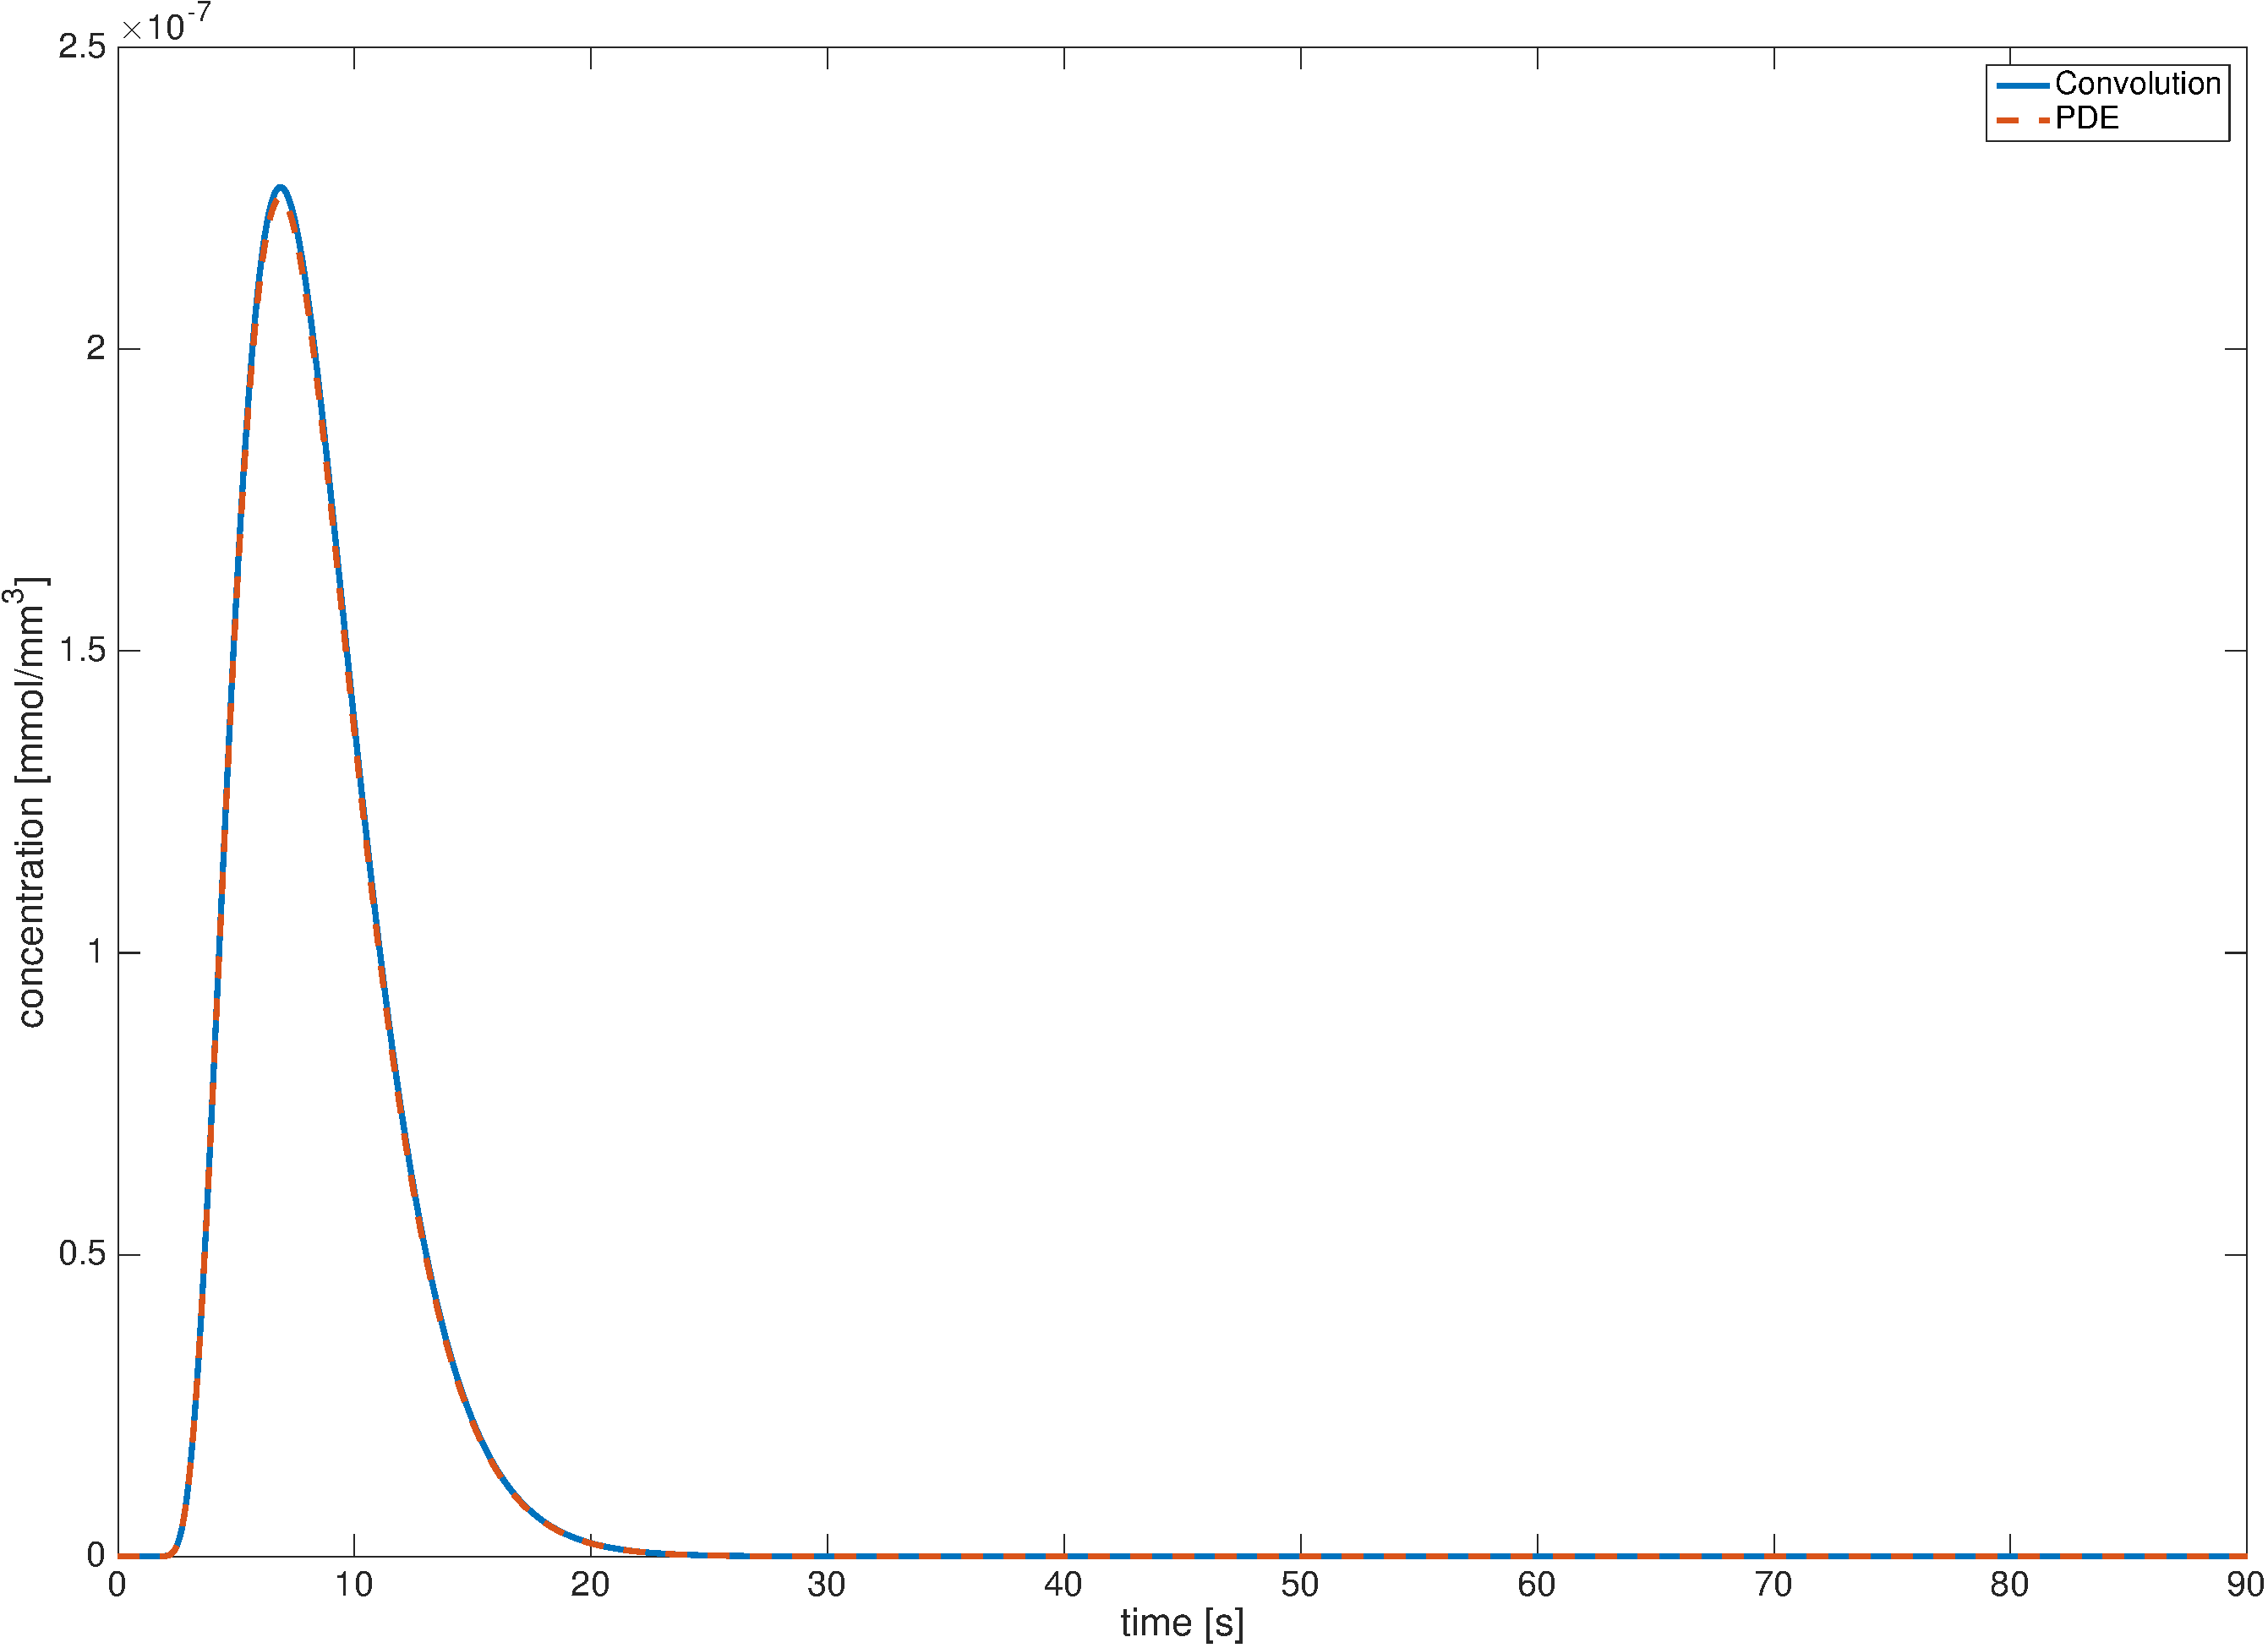
\includegraphics[width=.45\textwidth]{./figs/ConvVsPDE.pdf} \\
			a) Tissue curve at location [32,35]. Simulation using \eqref{eq:voxelcurve} (blue) and transport model (red).\\
			 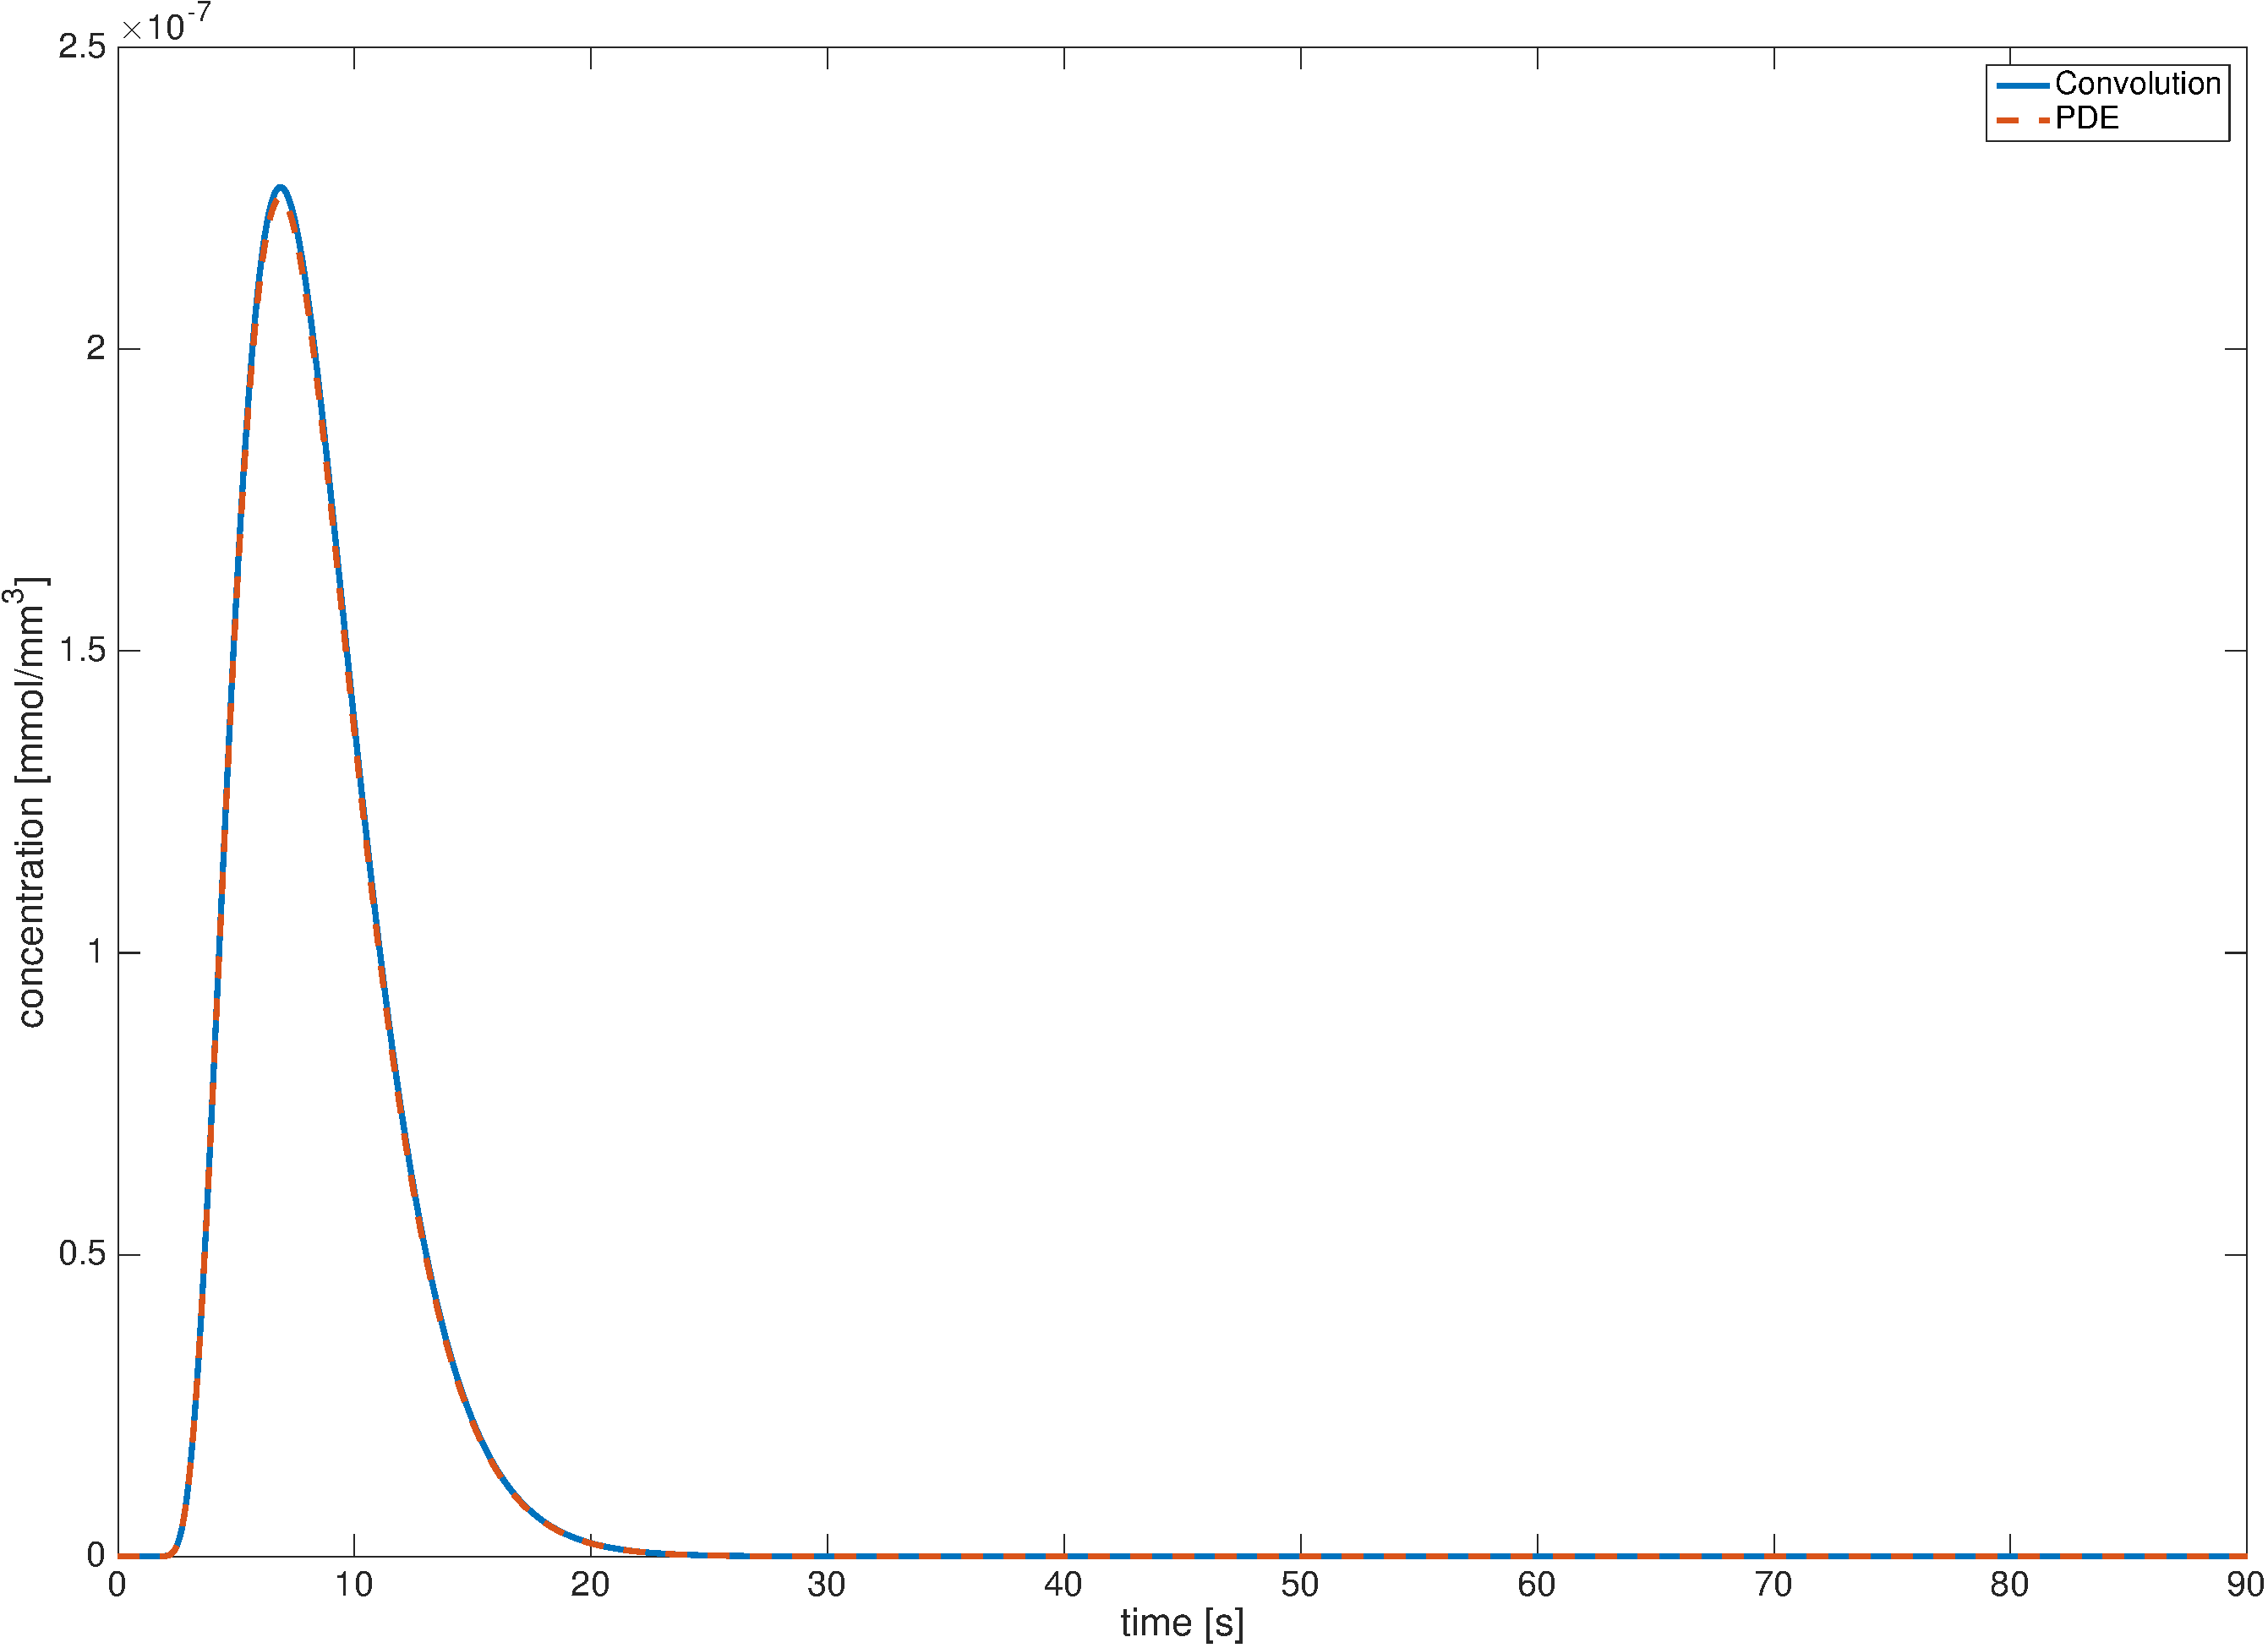
\includegraphics[width=.45\textwidth]{./figs/ConvVsPDE.pdf} \\
		\end{tabular}
		\caption{a) Tissue curve of the 2D phantom at location [32,35]. Simulation using \eqref{eq:voxelcurve} with $P_i=\SI{5328}{\siPml}$ and $c_{\mathrm{in}}$ taken locally from upstream voxels in blue and simulation using the transport model in red. Curves are coinciding perfectly. Note that the perfusion is unrealisticly high. b) Impuls response functions at location [1,20] for the global arterial input function. The analytic function given by \eqref{eq:IAna} is displayed in blue, the function recovered by deconvolution is displayed in red. As outlined in Section~\ref{sec:NewAndOld} both functions are coinciding perfectly. Note that the recovered impuls-response function depends on the perfusion of all upstream voxels and not only the adjacent voxels.}
	\end{figure}
	
	
	%--------------------------------------------------
	% Subsection: Relating New Model with Old Model
	%--------------------------------------------------
% \subsection{Relating the transport equation model with the traditional deconvolution model for perfusion}
% 	\label{sec:relating}
% 	Consider the solute transport equation (\ref{eq:conteqlocal}), and rewrite it as
% 	\begin{equation}
% 		\frac{\partial c}{\partial t} + \frac{q}{\phi} \cdot \nabla c = \frac{(c_{so}-c)Q_{so}}{\phi }.
% 		\label{eq:conteqlocal3}
% 	\end{equation}
% 	for a nonzero $\phi$, and where we used \eqref{eq:syntcontsimp2} and $Q = Q_{so} + Q_{si}$.
% 	We follow the method of characteristics and convert from Eulerian coordinates $(x(t),t)$ to Lagrangian coordinates $(x_0,t)$.
% 	Here $(x_0,t_0)$ corresponds to the beginning of a streamline at point $x_0$ and timepoint $t_0$.
% %	The parameterization parameter for the streamline emerging at $(x_0,t_0)$ is denoted by $s$.
% 	Substituting $x = x(t)$, and denoting $c(t):=c(x(t),t)$, $\Qso(t):=Q_{so}(x(t))$, $\phi(t):=\phi(x(t))$ and $c_a(t):=c_a(t)$  yields the following system of ODEs \cite{evans98}:
% 	\begin{subequations}
% 		\label{eq:ODEs}
% 		\begin{alignat}{2}
% 			\frac{Dc}{Dt} + \frac{\Qso(t)}{\phi(t)}c(t) &= \frac{c_{so}(t)\Qso(t)}{\phi(t)}, & \quad c(0) &= 0 \label{eq:ODEC} \\
% 			x'(t) &= \frac{q(t)}{\phi(t)}, &x(0) &= x_0 \label{eq:ODEx}\\
% 		\end{alignat}
% 	\end{subequations}
% 	The notation $Dc/Dt$ refers to the total derivative (material derivative) of $c$ with respect to the parameterisation $t$.
% 	The solution variable $c(t)$ can be regarded the concentration curve of a particle which originated at $(x_0,t_0)$ and where $(x(t),t)$ is the wavefront at time point $t$.
%
% 	Equation \eqref{eq:ODEC}, which governs the behaviour along the streamline, has the general solution
% 	\begin{equation}\label{eq:Sol}
% 		c(x(t),t) = \int_{0}^{t} e^{-(R(t)-R(s))}c_{so}(s)\frac{\Qso(s)}{\phi(s)} \diff s
% 	\end{equation}
% 	where $R(s)=\int_{0}^s\Qso(x(u))/\phi(x(u)) d u$.
%
% 	We now impose the additional assumptions that $\Qso$ and $\phi$ are constant along the streamline up to timepoint $t$.
% 	Following the path of a particle emerging at timepoint $t_0=0$, one can see that \eqref{eq:Sol} becomes
% 	\begin{equation}\label{eq:Cpdeclassic}
% 		C(x(t),t) = \Qso \int_{0}^t e^{-(t - s)/T}c_{so}(s) \diff s
% 	\end{equation}
% 	where $T := \Qso/\phi$ and $C = c \phi$.
% 	A comparison with \eqref{eq:traditionalperf} shows that these expressions are equal provided $Q_a = Q_{so}$ and $c_{so} = c_{a}$.
% 	We can interpret \eqref{eq:Cpdeclassic} as a so-called Lagrangian description of the the concentration of CA at a wave-front moving through a constant source-field, where at every voxel there is contribution of an arterial input.
% 	Note in contrast, that \eqref{eq:traditionalperf} is typically interpreted as an Eulerian description of contrast agent concentration at a fixed point in space.


	%--------------------------------------------------
	% Subsection: Converting Flow to Perfusion
	%--------------------------------------------------
	\subsection{Converting Flow to Perfusion}\label{sec:flux2perf}
	The model described in \eqref{eq:flowmodel} uniquely determines the flux field $q(x)$. 
	However, in pharmacokinetic modeling the parameter of interest is usually the CBF, which we will denote by $\Perf (x)$ as the voxel wise field of perfusion. The surface flux and perfusion are physically distinct, and there are at least two differences between $q(x)$ and $\Perf (x)$. 
	First, the flux is a vector field and the perfusion is a scalar field. 
	Second, the flux is normalized to a surface area and the perfusion is normalized to a volume. 
	Thus, the surface flux and the perfusion are strictly, mathematically different but still conceptually related. 
	In the following we describe a method for converting flux into perfusion, motivated by the need to compare the ground-truth flux field to the scalar valued perfusion field obtained by traditional methods. The other way around, converting perfusion into flux has no obvious incentive since the vector flux field contains both scalar and directional information compared to the scalar perfusion field.
	

	The common understanding of perfusion or volume flux $\Perf (x)$ is the amount of blood feeding a tissue volume per unit time, with units [\si{\siQmm}]. 
	For inter-subject comparison it is common to scale this quantity to normalized perfusion having units \si{\siPml}. 
	One obvious approach for converting flux into perfusion could be to estimate the perfusion as the total inflow (or outflow) of fluid (e.g. arterial blood) into a control region per unit time, and then normalizing with the control region volume. 
	This is a valid approach only if the control regions are not feeding each other, and is therefore well-founded 
	for the entire organ. 
	Such understanding of perfusion is in line with the theoretical foundation of traditional compartment models for perfusion where a control region has its own source of feeding arterial blood, independent of the neighbor regions. 
	
	On the other hand, if the control region is a single voxel or a sub-division of an organ with sequentially feeding arterial blood, the traditional model assumptions are violated since every control region will feed its neighbours, thus becoming a coupled system of flow. 
	Simply summing the total inflow into a voxel and dividing by the voxel volume will strongly over-estimate the perfusion since the normalization would refer to the wrong volume. 
	The problematic issue is that the incoming blood is feeding more ROIs than the current ROI, and the perfusion values thereby become discretization dependent. 
	This phenomenon is demonstrated in Fig. \ref{fig:perfusion-problem} where the volume on the left has the true perfusion of $\Perf_{1} = \Flow_0 /(2V)$ for an incoming flow $\Flow_0$ [$\si{\siFmm}$] and distribution volume $2V$ [$\si{\simm}$]. 
	However, for another discretization as shown in the middle, the perfusion within each of these sub-volumes becomes $\Perf_{2} = F_0/V = 2\Perf_{1}$. 
	Taking the average across the two sub-volumes, it is clear that the perfusion is over-estimated with a factor of two. 
	A discretization dependent perfusion estimate is not recommendable, and the perfusion estimate of $\Perf_{2}$ is clearly wrong. 


	\begin{figure}[H]
	    \centering
	    \begin{overpic}[scale=0.3]{figs/perfusion-problem.eps}
	    	\put(11,70){\color{black}$F_0$}
			\put(49,70){\color{black}$F_0$}
			\put(85.0,70){\color{black}$\Delta F_0$}
			\put(13,33){\color{black}$2V$}
			\put(50,20){\color{black}$V$}
			\put(50,45){\color{black}$V$}
			\put(91,42){\color{black}$\Delta V$}
		\end{overpic}
	    \caption{Perfusion within a small volume. Left: A compartment with volume $2V$ is exposed to a flow $\Flow_0$ [$\si{\siFmm}$] of fluid. By definition, the perfusion within this compartment becomes $\Perf_{1} = \Flow_0/(2V)$. Middle: The same volume is divided into two compartments (e.g. voxels), and the perfusion for each of the compartments becomes $\Perf_{2} = \Flow_0/V = 2\Perf_{1}$. The discrepancy between the two discretizations occurs because the flow is counted twice as it is fed from one voxel to the other. Right: As a solution to the described problem we rather pick out a true distribution volume $\Delta V$ (area in this 2D sketch), which is a small area around a given streamline along the centre line of the grey area. This is the true distribution volume (area in this 2D sketch) which is fed with arterial blood from the incoming fractional flow $\Delta \Flow_0$. The correct perfusion within $\Delta V$ is therefore $\Delta F_0/\Delta V$. The entire compartment can further be divided into similar infinitesimal distribution volumes, thus providing locally correct perfusion estimates.}
	    \label{fig:perfusion-problem}
	\end{figure}

	The reason for the discrepancy is that $\Perf_{2}$ has been counted twice since the voxels are coupled and we are dividing by the wrong distribution volume. 
%	Instead, we need to consider the traditional definition of perfusion. 
	The concept of perfusion has a very precise meaning, as the amount of arterial blood per time unit delivered to a capillary bed in a biological tissue, and then scaled by the fed tissue volume. 
	Therefore, the incoming flow must be divided by the total distribution volume that is covered by the fluid streamlines. 
	This formulation coincides with the traditional understanding of perfusion, and the correct distribution volume will rather be the volume that the fluid particles within an infinitesimal cross-sectional area around the streamlines are covering. 
	Assuming laminar flow, the streamlines are not crossing each other and we can estimate the true distribution volume that is fed by a given arterial blood flow.

	Let us fix a point $y(s) \in \Omega$ and consider the streamline passing through $y(s)$ for a parameterization $s$ along the streamline, such that $s \in [0,L]$, where $L$ is the length of the streamline passing through $y(s)$. For the time being, denote the flux along this streamline as $q = q(s)$, noting that the direction of the streamline is identical to the direction of the flux.
	Let $A(s)$ be the area of a 2-D infinitesimal small element $\mathbb{A}(s)$ of arbitrary shape surrounding the streamline at position $y(s)$, where any in-plane vector of $\mathbb{A}(s)$ is orthogonal to $q(s)$, and also such that the boundary of $\mathbb{A}(s)$ will never intersect any streamline upon moving $\mathbb{A}(s)$ along the streamlines for varying $s$. This is possible to achieve for a laminar flow field where streamlines will never cross.
	Due to mass balance, the volume flow [\si{\siFmm}] across $\mathbb{A}(s)$ is independent of position along the streamline, and can for any value of $s$ be expressed as
	\begin{equation}
		F(s) = ||q(s)|| A(s)
	\end{equation}
	assuming the area element $\mathbb{A}(s)$ is sufficiently small such that $q(s)$ can be considered constant across $\mathbb{A}(s)$. This is a reasonable assumption as we will later let $A(s) \rightarrow 0$.
	The outer boundaries of the distribution volume for the fluid is aligned with the streamlines, and can in terms of absolute values be expressed as
	\begin{equation}
		V = \int_0^L A(s) ds.
	\end{equation}
	Hence, according to definition of perfusion \cite{Petrella2000}, we can express the perfusion $\Perf$ acting within $V$ for any position along the streamline as
	\begin{equation}
		\Perf(s) = \frac{F(s)}{V} = \lim_{A(s) \rightarrow 0}\frac{||q(s)||A(s)}{\int_0^L A(s)ds} = \frac{||q(s)||}{L}
		\label{eq:flux2perf}
	\end{equation}
	upon letting $A(s) \rightarrow 0$ and applying L'Hopital's rule.
%	Consider now a (unique) streamline passing through $y$ of length $L$ as well as a small tube of radius $\varepsilon(s)$ around the streamline where $s$ is a parameterisation along the streamline. 
%	Provided $q$ is continuous along the streamlines, we know $\exists ~ \tilde{\varepsilon}, 0 \leq \tilde{\varepsilon} \leq \max_s \varepsilon(s)$, such that the volume $V$ of the tube can be expressed as $V = \tilde{\varepsilon}^2\pi L$
%	Hence we can express the perfusion $\Perf_{\varepsilon}$ for the sub volume $V$ as
%	\begin{equation}
%		\Perf_\varepsilon = \frac{F}{V} = \frac{1}{\tilde{\varepsilon}^2 \pi L} \int_{A_{\tilde{\varepsilon}}} \left( q\cdot \frac{q}{\Vert q \Vert} \right) \diffint A. 
%		\label{eq:Pneps}
%	\end{equation}
%%	Letting $\tilde{\varepsilon} \to 0$ and using the relation $F/(\tilde{\varepsilon}^2\pi) \rightarrow \Vert q \Vert$ provided $q$ is continuous, 
%Upon integration, this yields a locally defined value for the perfusion $\Perf (y)$
%	\begin{equation}
%		\Perf(y) = \frac{\Vert q(y) \Vert}{L}.
%		\label{eq:flux2perf}
%	\end{equation}
	%We note that \eqref{eq:Pneps} is valid for any $0 \leq \tilde{\varepsilon} \leq \max_s \varepsilon(s)$ since both $F$ and $V$ are independent of $\varepsilon$, and relation \eqref{eq:flux2perf} is thereby valid for any position along the streamline.
	Equation \eqref{eq:flux2perf} is an explicit formula for converting flux into perfusion and is later used to enable a comparison between the traditional model for perfusion and a corresponding ground-truth flux field. 
	
	
	


	%--------------------------------------------------
	% Subsection: Estimate the Porosity
	%--------------------------------------------------	
	\subsection{A Method to Estimate local Porosity}\label{sec:CBV}
	
	It is known from literature on traditional models for perfusion that CBV for the entire compartment can be expressed as
	\begin{equation}
		\phi = \frac{\int_0^\infty C(t) dt}{\int_0^\infty c_a(t) dt}.
		\label{eq:CBV}
	\end{equation}
	where $C(t)$ are the tracer concentration with respect to a well mixed compartment and $c_a(t)$ is the tracer plasma concentration of the arterial input.
	However, it is not obvious that \eqref{eq:CBV} is valid also for a continuous field model where the voxels are feeding each other. We will now proof that \eqref{eq:CBV} is nevertheless valid.
	
	% mass balance of fluid and tracer particles is described by \eqref{eq:flowmodel} and \eqref{eq:conteqlocal}. 
	Returning to the local definition of fluid tracer concentration as $c(x,t)$, the PDE in \eqref{eq:conteqlocal} is consistent with
	\begin{equation}
		\phi\frac{\partial c}{\partial t}  = - q \cdot \nabla c.
		\label{eq:1cmodel}
	\end{equation}
	for locations $x$ where $Q(x) = 0$.
	Integrating from $t_0$ to $t_1$ results in the model
	\begin{equation}
		\phi [c(x,t_1) - c(x,t_0)]  = - \int_{t_0}^{t_1}q \cdot  \nabla c \diffint t.
	\end{equation}
	Approaching the limit $t_0 = 0, t_1 = \infty$, using the boundary conditions $c(x,0) = c(x,\infty) = 0$ and defining $E(x):= \int_0^\infty c(x,t) \diffint t$ leads to
	\begin{equation}
		0 = q \cdot \nabla  E(x).
		\label{eq:streamlinezero}
	\end{equation}
	We can interpret this equation such that $q$ lies parallel with the level-sets of the function $E(x)$, which means that $E(x)$ is constant along the streamlines of the fluid flow, and thereby also valid when approaching the source $\Omega_{Q_{so}} = \{x: Q_{so}(x) > 0\}$ along the streamlines:
%	Since we assumed that $Q$ has a delta-like structure and since all streamlines are emerging at the arterial-input, we obtain
	\begin{equation}
		\int_0^\infty c(x,t) \diffint t = \lim_{x \rightarrow \Omega_{Q_{so}}}\int_0^\infty c(x,t) \diffint t.
	\end{equation}
	Using $C(x,t) = \phi(x) c(x,t)$ we obtain
	\begin{equation}
		\phi(x) =  \frac{ \int_{0}^{\infty} C(x,t) \diffint t }{\lim_{x \rightarrow \Omega_{Q_{so}}} \int_{0}^{\infty} c(x,t) \diffint t}.
		\label{eq:phi}
	\end{equation}
	For all practical applications with a source field $\Omega_{Q_{so}}$ of limited extension and homogeneous and simultaneous CA input one can replace the denominator by $\int_0^\infty c_a(t) \diffint t$.
	Equation \eqref{eq:phi} for porosity coincides with the traditional formula \eqref{eq:CBV} for $\phi$ and is hereby proven analytically also for local estimations of the porosity $\phi$.
	
	


	

	%--------------------------------------------------
	%--------------------------------------------------
	% Section: Numerical implementation
	%--------------------------------------------------
	%--------------------------------------------------
	




	%--------------------------------------------------
	%--------------------------------------------------
	% Section: Experiments
	%--------------------------------------------------
	%--------------------------------------------------
	\section{Numerical Experiments}\label{sec:NumExp}
Based on the field modes described in Section \ref{sec:synthetic}, we now establish an experimental setup suited to study the performance of the deconvolution methods in a synthetic flow field with a known ground truth.

	\subsection{Parameter settings}
	Based on \eqref{eq:flowmodel} and \eqref{eq:conteqlocal} we set up a forward simulation of blood-flow and indicator dilution through the capillary system. We aimed at creating a transparent synthetic test case and kept all optional parameters as simple as possible. 
	Therefore, permeability and porosity were assumed constant in space and in time. The source term was assigned to the upper left voxel and the sink term was assigned to the lower right voxel. 	We chose a standard arterial input function \cite{ostergaard96}, a gamma-variate \cite{chan04} function
	\begin{equation}
		\ca(t) := D_0(t-t_0)^\alpha e^{-(t-t_0)/\beta}
	\end{equation}
	for $\alpha=3$, $D_0 = 1$, $\beta = \SI{1.5}{\second}$ and $t_0 = \SI{0}{\second}$.

	An overview of parameter settings used for the numeral simulations are shown in Table \ref{tab:par}. Total inflow within the source is denoted $F_{so} = \int_\Omega Q_{so}(x) dx$, and similarly for the sink $F_{si} = \int_\Omega Q_{si}(x) dx$. We chose an average input perfusion of $50$\si{\siPml}, which can be converted into a flow of $F_{so} = 0.83$ \si{\siFmm} for the closed domain $\Omega = \{x = (x_1,x_2,x_3) : 0 \leq x_1 \leq 10mm, 0 \leq x_2 \leq 10mm, 0 \leq x_3 \leq 1 mm\}$.
	\begin{table*}[]
	\scriptsize
		\centering
	  \caption{Parameters used in the numerical experiments, optimized for a slab of the capillary system in the human brain. In order to achieve a transparent simulation, permeability was assumed to be isotropic, and both permeability and porosity were assumed to be constant across the domain. A typical porosity of $\phi = 0.05$ was chosen \cite{Smith00}.}		
		\begin{tabular}{ l  c  c c  r }
		    Description 							&	Type 	& Symbol 			& Value(s) 				& Unit 				\\
			\toprule
			Surface flux 							&	Vector 			& $q$				& - 					& \si{\siq} 		\\
		         Average perfusion within $\Omega$		 &	Scalar & $\overline{\Perf}$ 	& $50$ 					& \si{\siPml}		\\
		         Volume flux/perfusion							 &	Scalar & $\Perf$ 	& - 					& \si{\siQmm}		\\
			Absolute flow in source, derived from $\overline{\Perf}$& 	Scalar	& $F_{so}$ 			& \num{0.83}			& \si{\siFmm} \\
			Absolute flow in sink 						&		Scalar		& $F_{si}$ 			& $-F_{so}$ 		 	& \si{\siFmm}  		\\
			Volume flux in source, derived from $F_{so}$& 	Scalar	& $Q_{so}$ 			& \num{34.13}			& \si{\siQmm} \\
			Volume flux in sink 						&		Scalar		& $Q_{si}$ 			& $-Q_{so}$ 		 	& \si{\siQmm}  		\\
			Concentration w.r.t. fluid space			&	Scalar & $c$				& - 					& \si{\sic} 		\\
			Concentration w.r.t. $\Omega_i$		&	Scalar 			& $C$				& - 					& \si{\sic} 		\\
			% Dynamic viscosity blood \cite{rosencranz06} 	& Scalar & $\mu_b$ 			& $\num{5e-6}$ 			& \si{\simu}  	\\
			Fluid density blood \cite{kenner89} 			& Scalar & $\rho$ 			& $\num{1}$				& \si{\milli\gram\per\cubic\milli\meter} 		\\
			Permeability  							&	Scalar	& $k$ 				& $\num{5e-6}$ 			& \si{\square\milli\meter} 			\\
			Porosity / CBV	\cite{Smith00}						&	Scalar	& $\phi$ 			& $0.05$ 				& \si{\cubic\milli\meter\per\cubic\milli\meter}	\\
			Spatial resolution 						&	Vector	& - 				& $(64,64,1)$ 			& -					\\
			Physical FOV 							&	Vector & - 				& $(10,10,1)$ 			& \si{\milli\meter}				\\
			Voxel size 							&	Vector	& - 				& $(0.156,0.156,1)$ 	& \si{\milli\meter}	\\
	  \end{tabular}
	  \label{tab:par}
	\end{table*}	
	
	Implementation details of \eqref{eq:flowmodel} and the transport equation \eqref{eq:conteqlocal} can be found in Appendix \ref{sec:numsynt}.

%	To solve \eqref{eq:flowmodel} we used the two-point flux approximation finite volume method (TPFA) \missingsource. 
%	The transport equation \eqref{eq:conteqlocal} was solved by first order upwinding \cite{Patankar80} applied to \eqref{eq:conteq}.
	\subsection{Indicator dilution in the porous media and the convolution model}


From the porous media model using  \eqref{eq:flowmodel} and \eqref{eq:conteqlocal}, streamlines were found from tracking of the flux vector field $q$, using a method closely related to FACT \cite{Mori1998} used for tracking within DTI (Diffusion Tensor Imaging) for tractography. Both length and position of the streamlines was during the tracking process assigned. The voxel-wise perfusion field $\Perf$ was calculated according to $\eqref{eq:flux2perf}$ using the computed streamline length and the flux field $q$ from \eqref{eq:syntdarcysimp}. The pressure field, the flux and voxel wise perfusion is displayed in Fig. \ref{fig:flowpressureperfusion}. The flow field visualized in  Fig. \ref{fig:flowpressureperfusion} (b) is vector flux integrated across cell surface, $\int_{\partial \Omega_{ij}}q ds$  with units [\si{\siFmm}].

		\begin{figure*}[]
		\centering
		\begin{tabular}{c c c}
			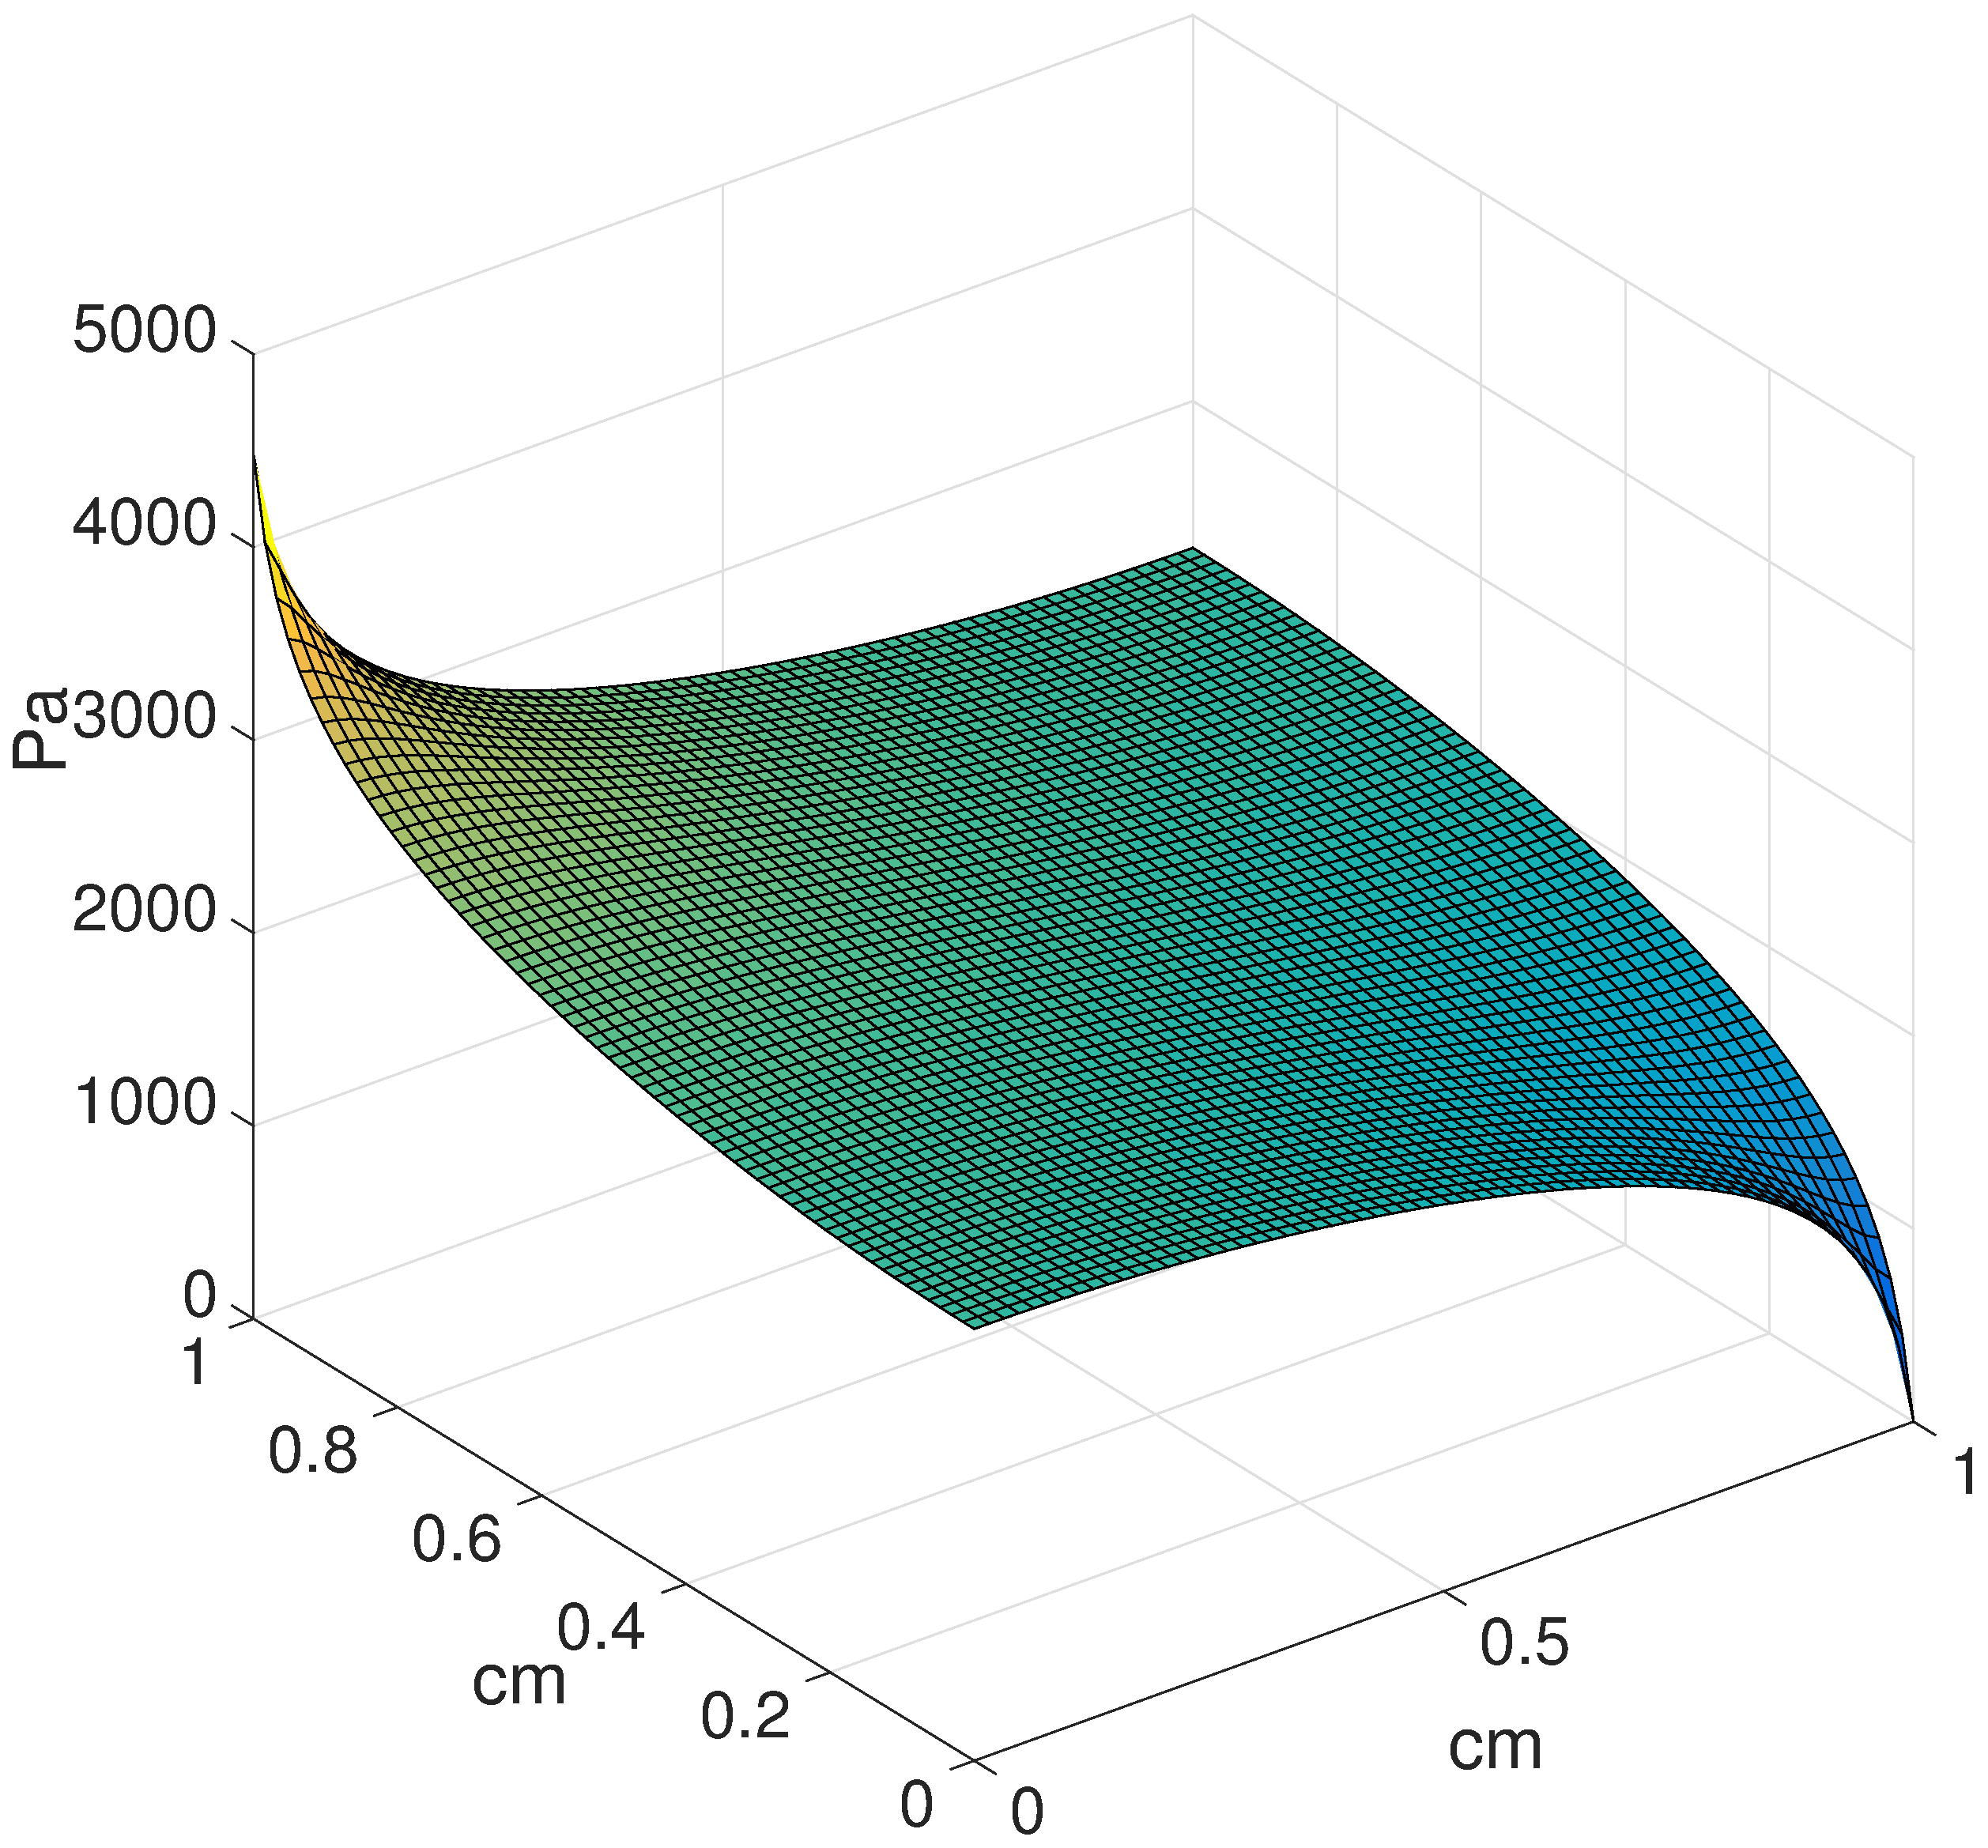
\includegraphics[width=.3\textwidth]{figs/pressure.eps} & 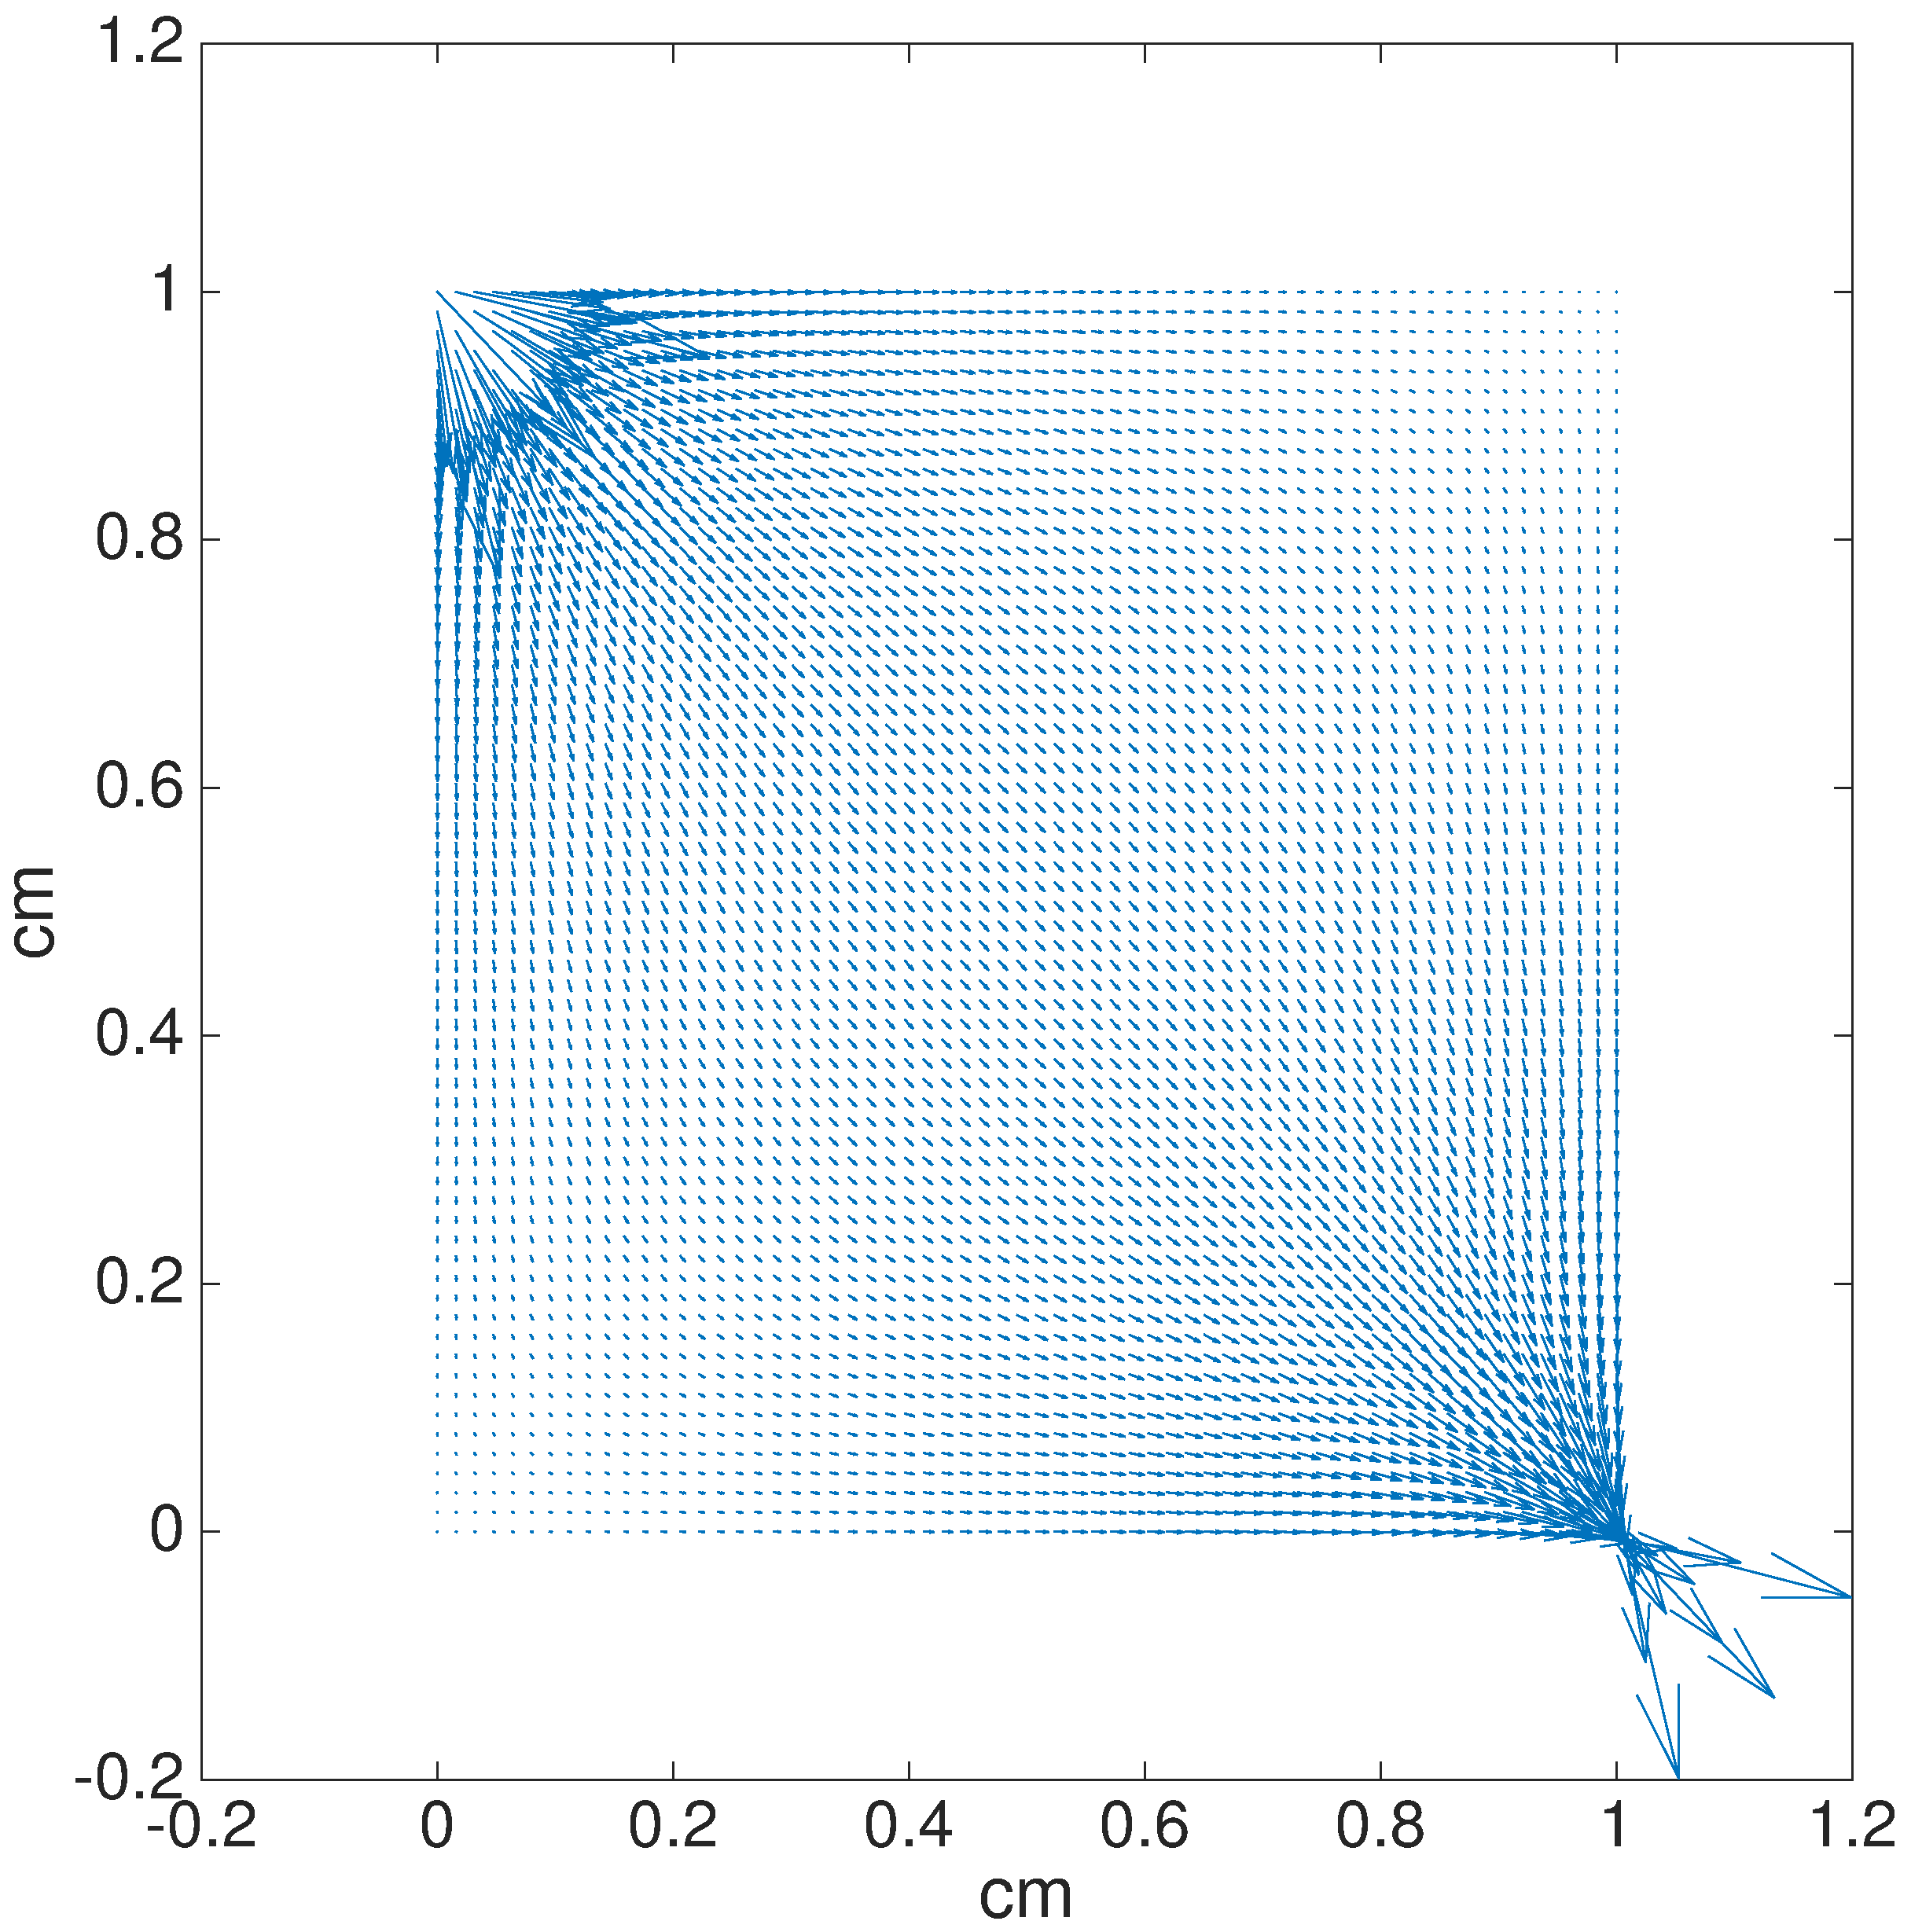
\includegraphics[width=.3\textwidth]{figs/flowQuiver.eps} & 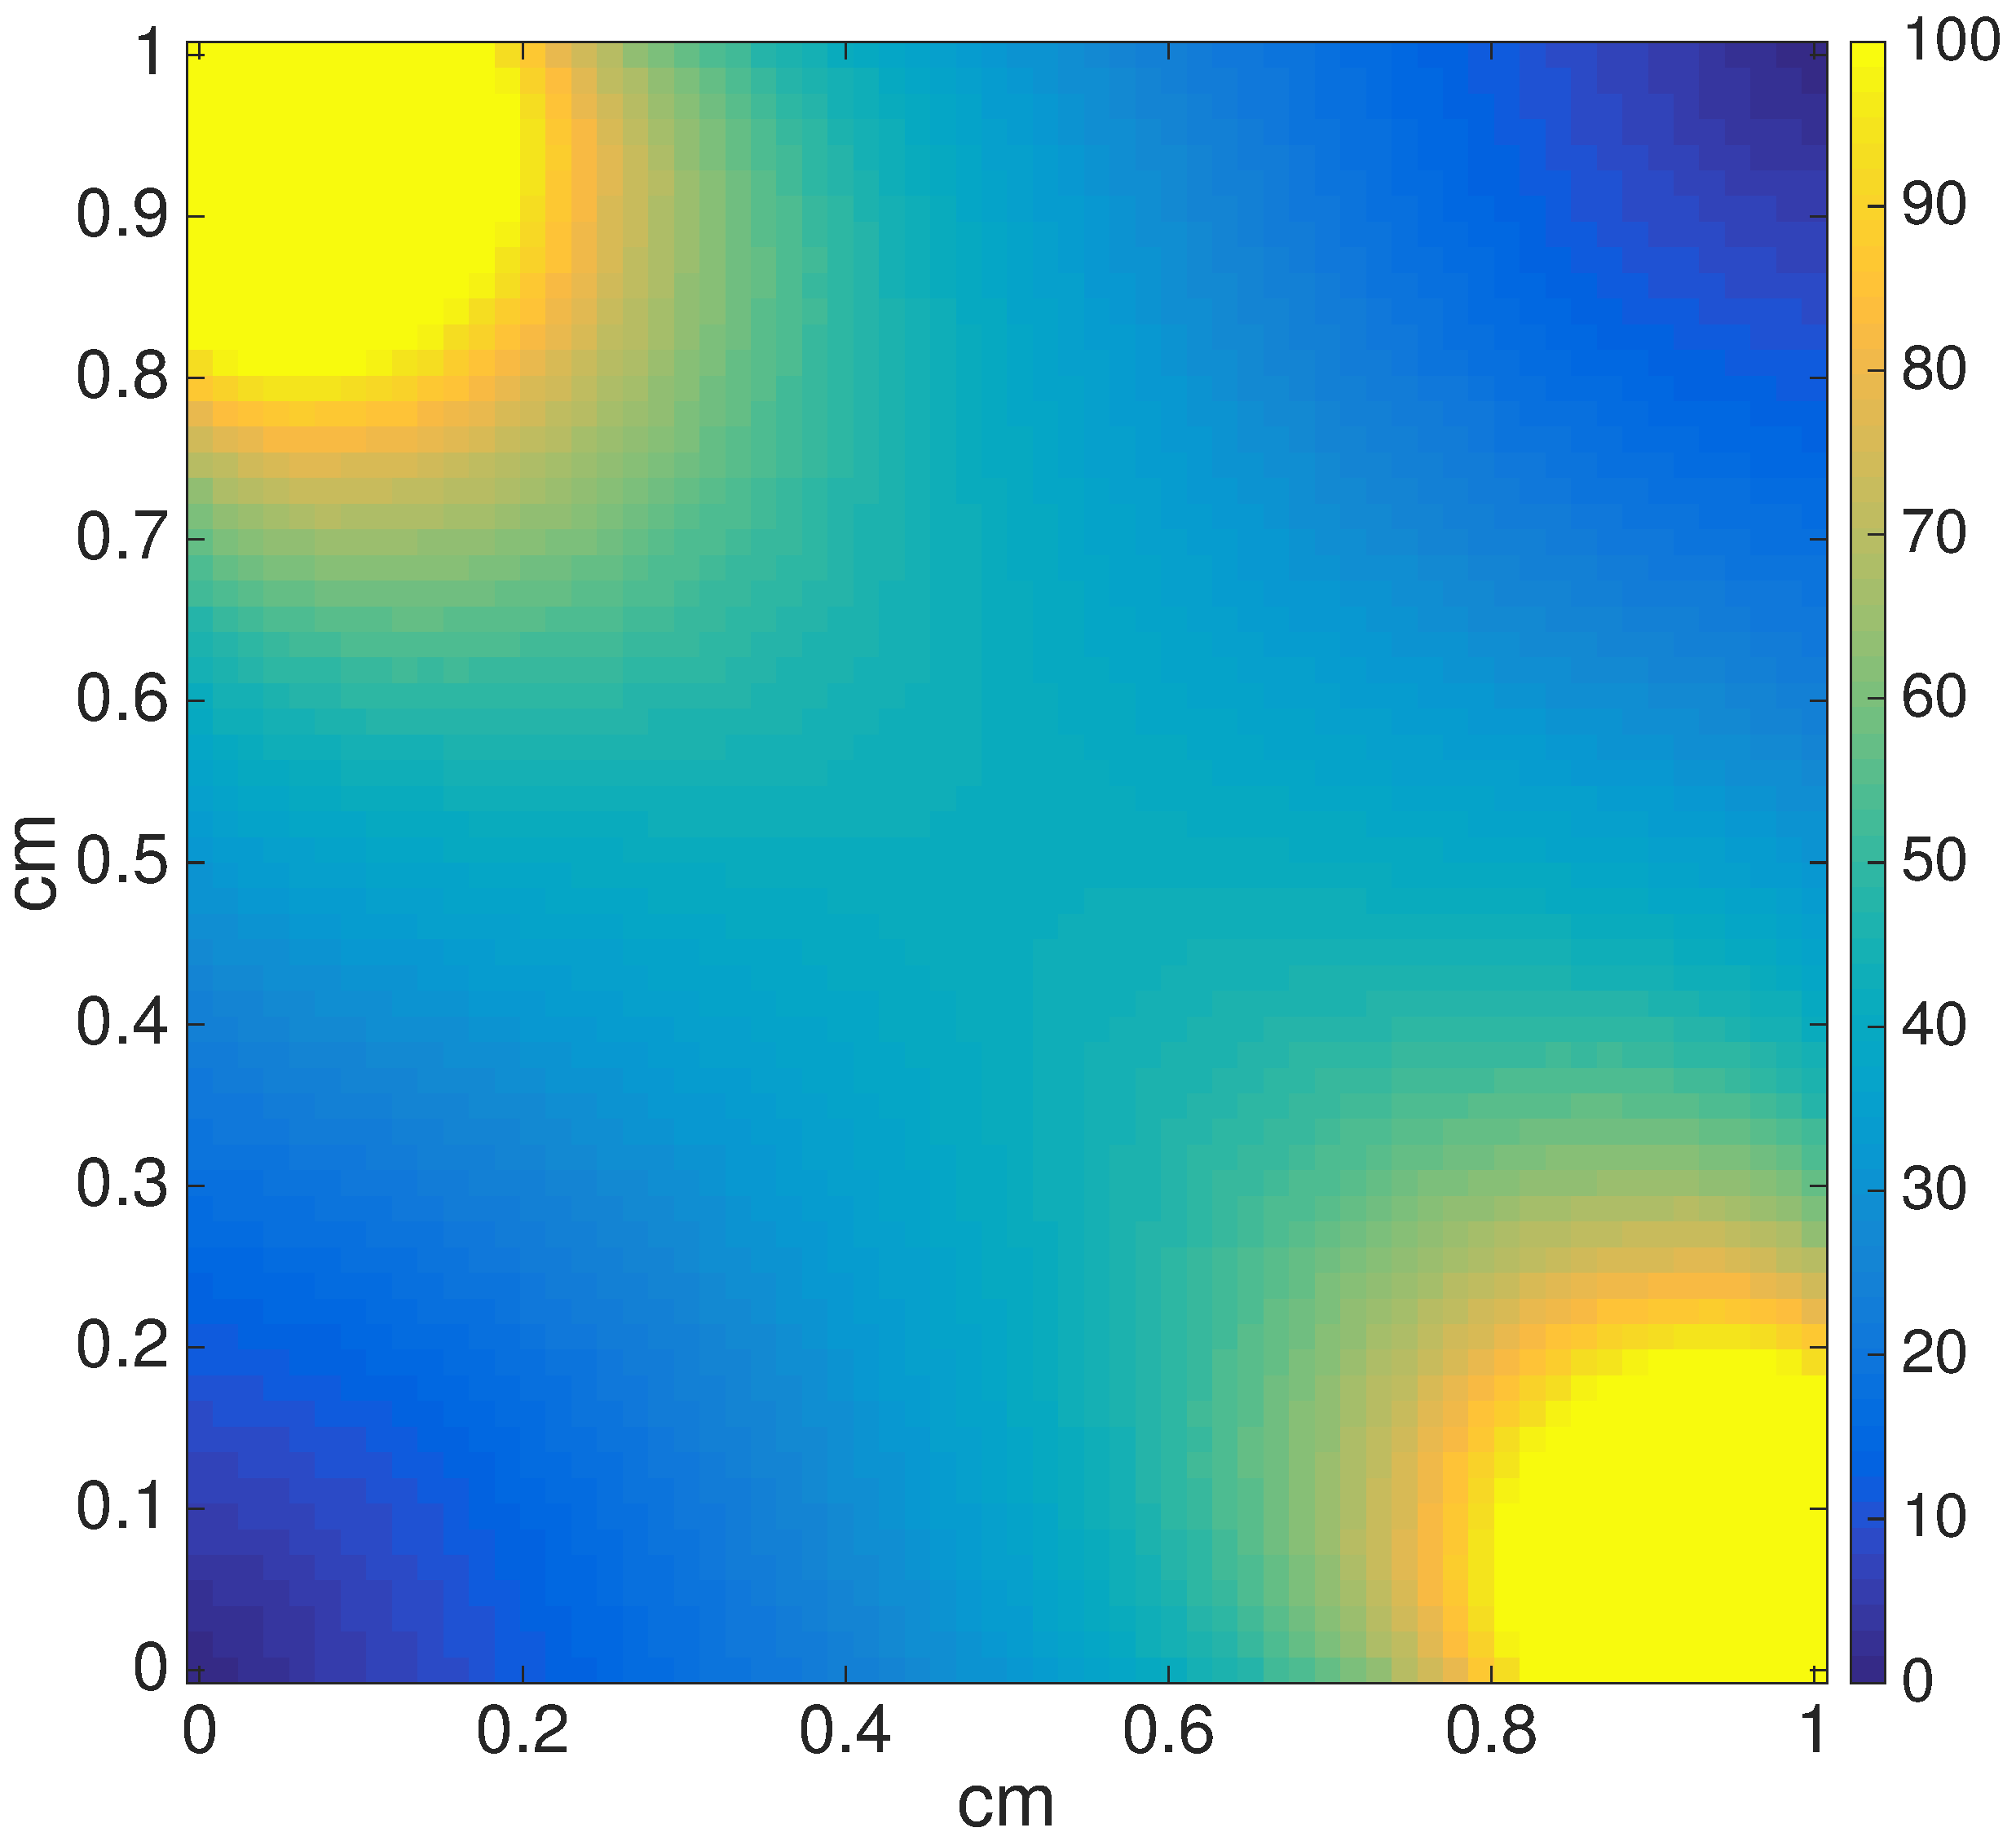
\includegraphics[width=.3\textwidth]{figs/perfusion.eps}\\
			(a) Pressure field $p(x)$ & (b) Flow field & (c) Perfusion field $\Perf(x)$.
		\end{tabular}
    	\caption{Porous media (PM) flow model with a source in the upper left corner and a sink in the lower right corner. (a) Pressure field [\si{\pascal}] from solving the linear system in \eqref{eq:flowmodel} , (b) Flow field $\int_{\partial \Omega_{ij}}q ds$ [\si{\siFmm}], (c) Voxelwise perfusion $\Perf(x)$ [\si{\siPml}] according to \eqref{eq:flux2perf}. Averaging of $P(x)$ yielded an average perfusion of $49.92$ \si{\siPml}, close to the input value of $50$ \si{\siPml}, serving as an internal control of the implementation of TPFA and the flux to perfusion conversion.}
	        \label{fig:flowpressureperfusion}
	\end{figure*}

	Maps of CA concentrations were computed by two means. (i) First, by simulating the transport equation \eqref{eq:conteq}, and (ii) second by the forward convolution model \eqref{eq:traditionalperf}. For (i), known values of flux, porosity, fluid density, and fluid flow within the source and sink were fed into the equation. We refer to this map as $C_T(x,t)$. For the forward convolution model (ii), the estimated voxelwise perfusion $\Perf_i$ and the porosity were used for the simulations with known values of $\Perf_a \leftarrow \Perf_i$. We refer to this map as $C_C(x,t)$. 
	A comparison of the tissue curves between $C_T(x,t)$ and $C_C(x,t)$ at different positions of the tissue can be found in Figure \ref{fig:tissuecomp}. 
%	In order to compare the porous media (PM) model to the forward convolution model Section \ref{sec:conv}, another CA dataset in addition to the PM model was generated using \eqref{eq:traditionalperf} and the known values of $\Perf_a \leftarrow \Perf_i$ as the perfusion for each voxel $i$.
%	The convolution dataset of CA intensities (convM) was set up assuming voxel-wise well-mixed compartments and the perfusion values described in \eqref{eq:flux2perf}.
%	Note that this assumption is in contradiction to the assumptions of the maximum-slope model.
	Note that the convolution dataset was set up under the assumption that each voxel is a well-mixed compartment.
	Since one assumption of the maximum-slope model is that no outflow takes place during the peak of the AIF, we cannot expect the maximum slope model to recover perfusion on a voxel basis for $C_C(x,t)$.

	\begin{figure*}[]
		\centering
		\begin{tabular}{c c}
			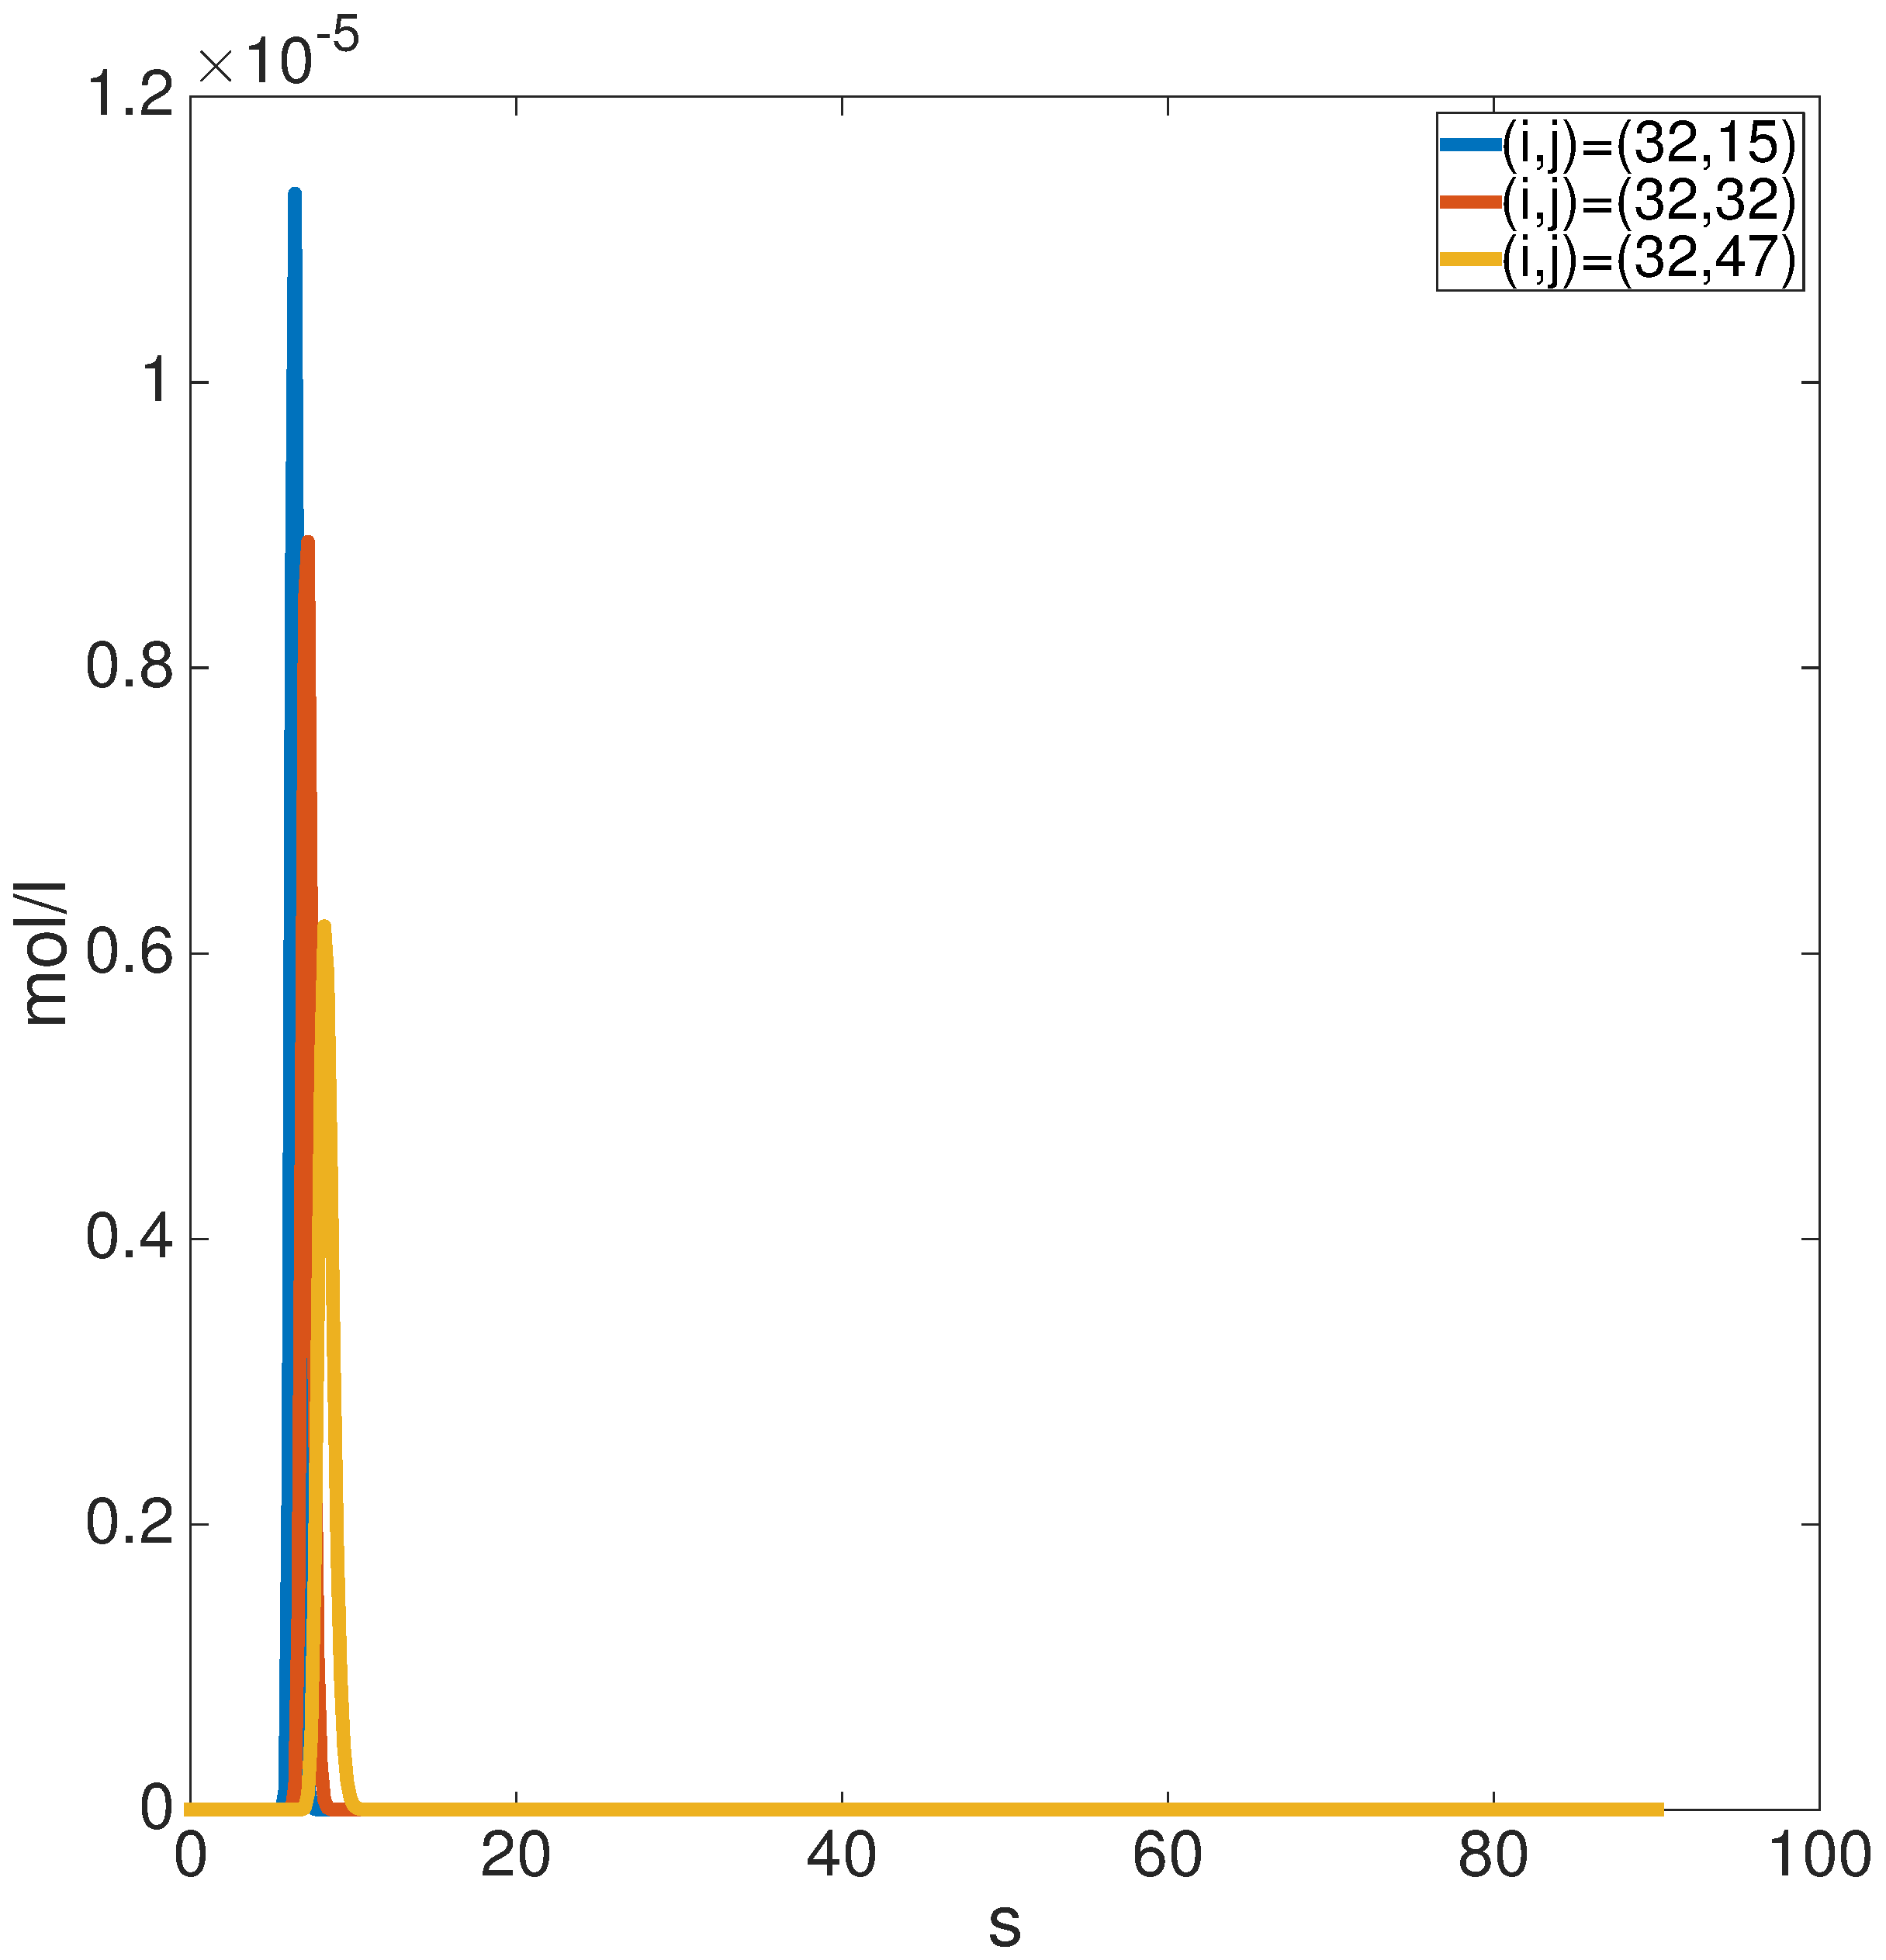
\includegraphics[width=.40\textwidth]{figs/PMM153247.eps} & 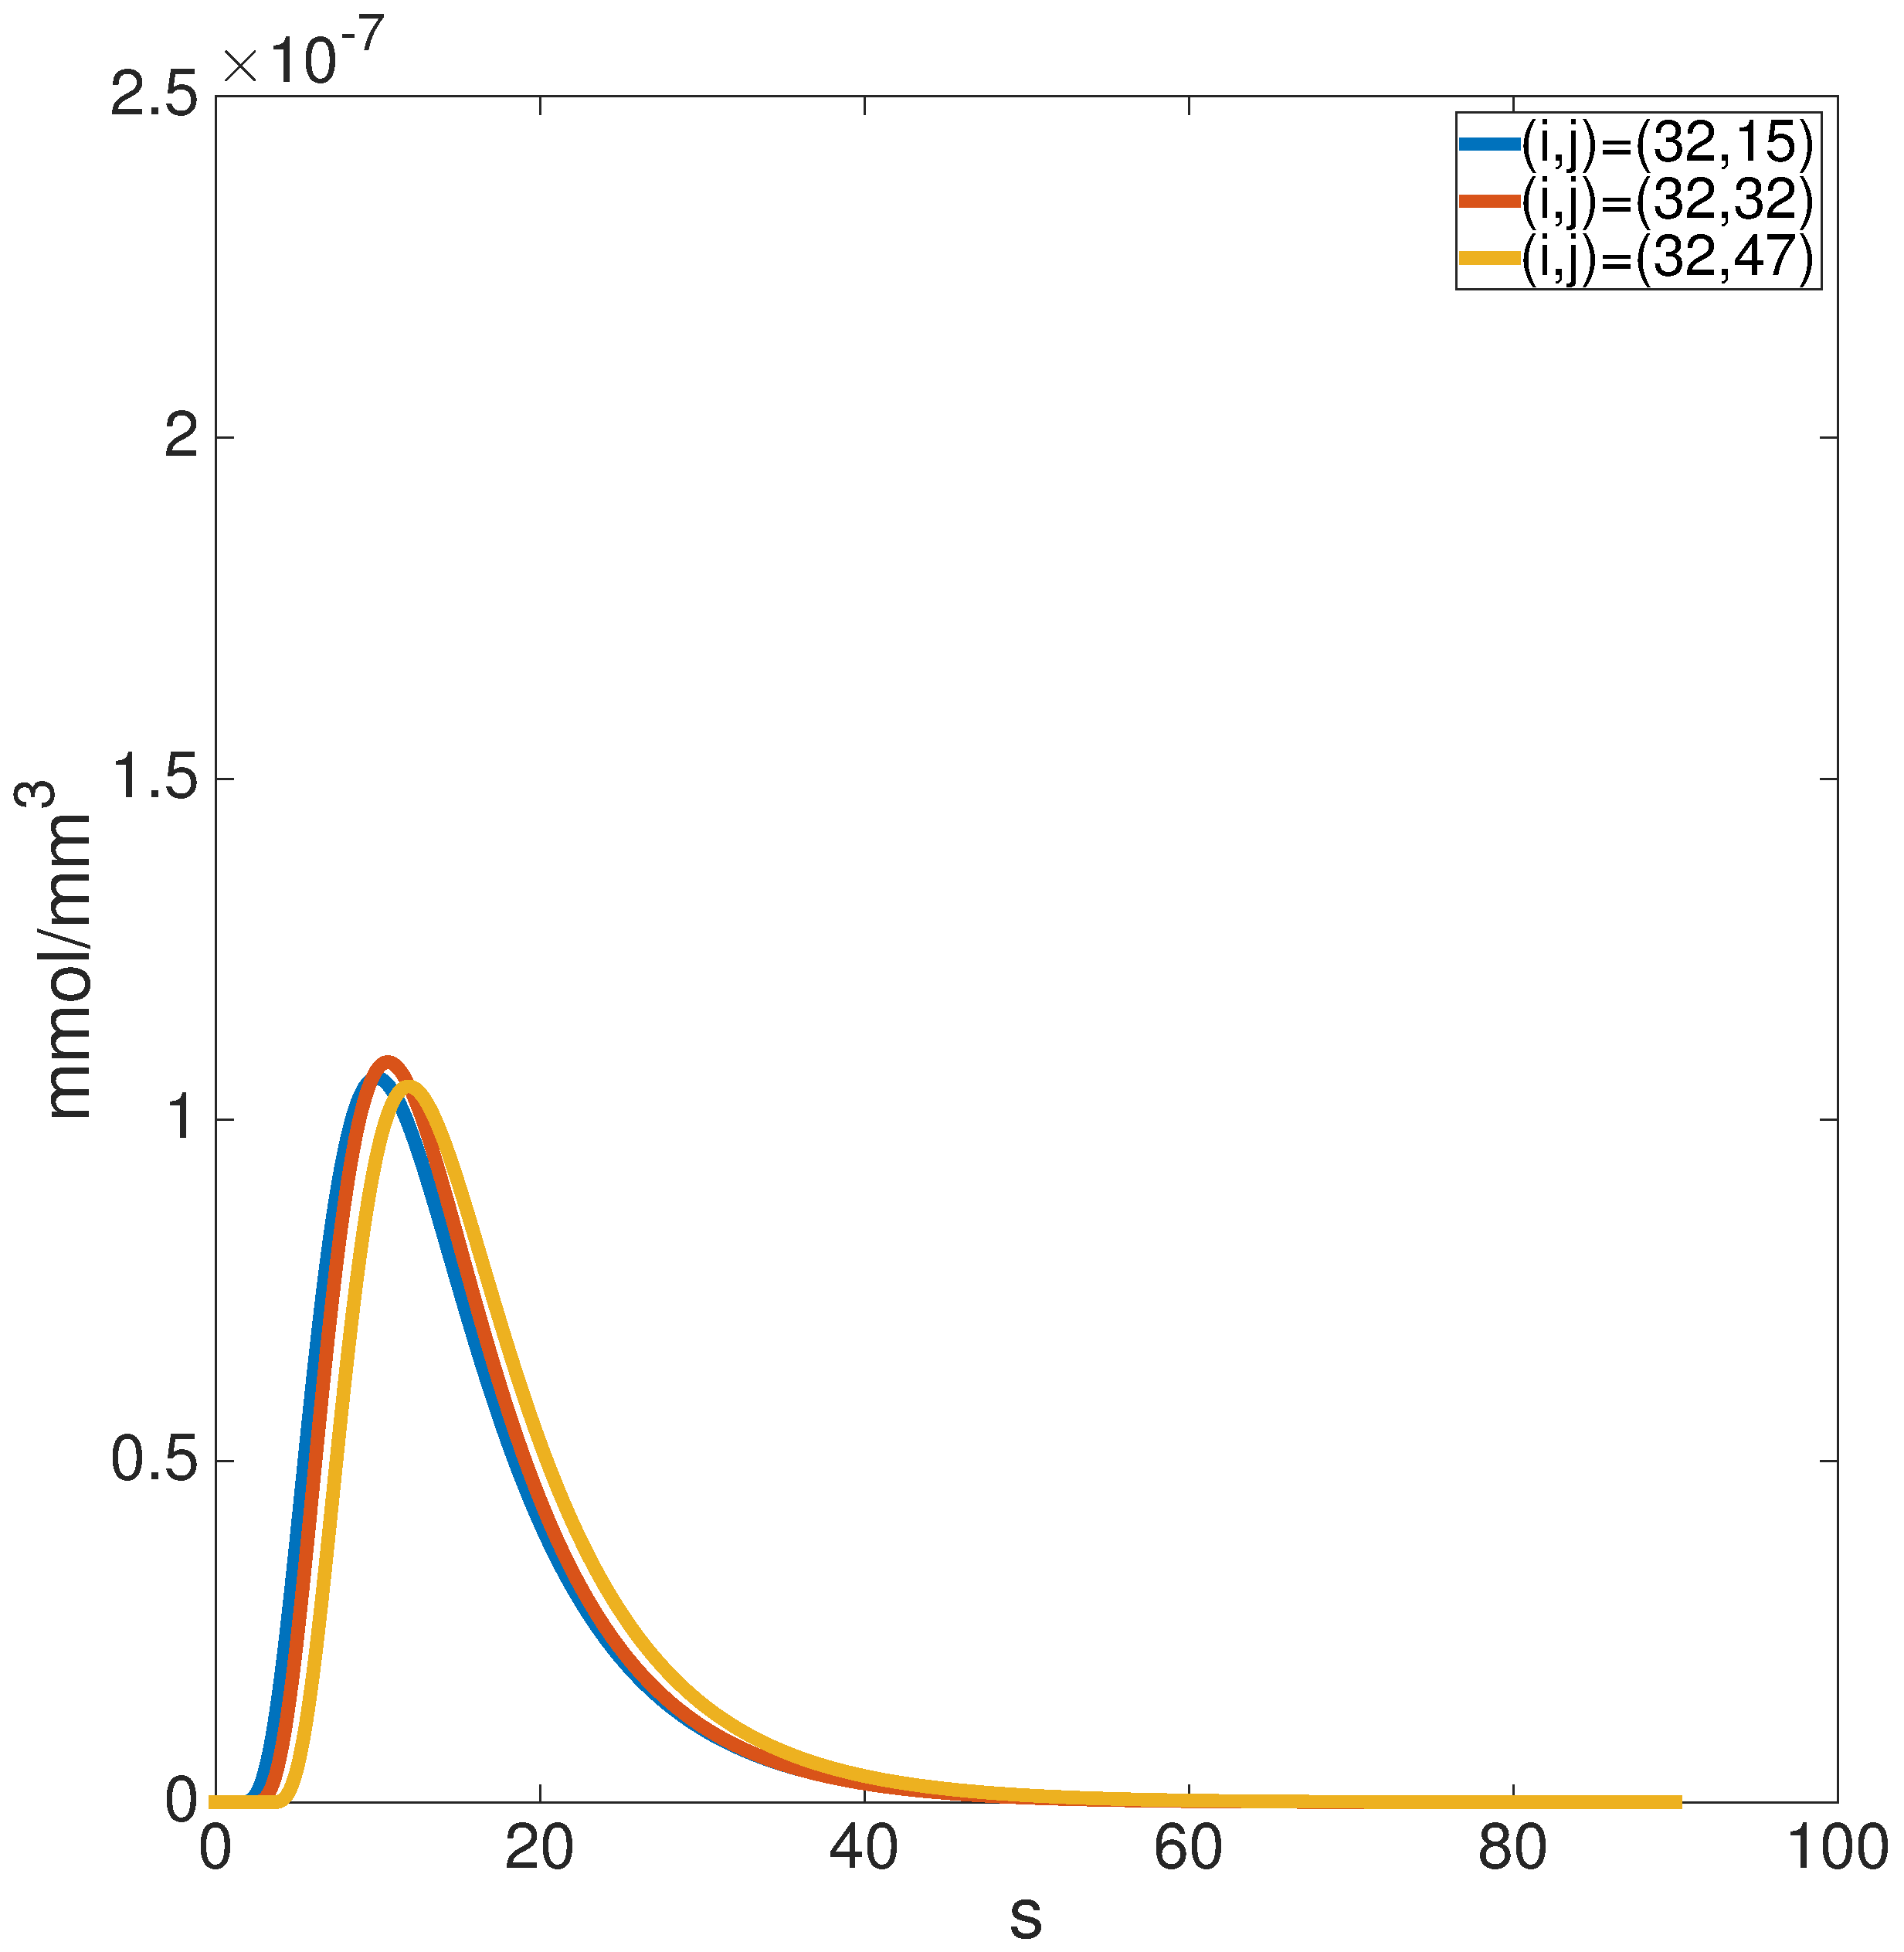
\includegraphics[width=.40\textwidth]{figs/convM153247.eps} \\
			(a) Transport equation $C_T(x,t)$ & (b) Convolution model $C_C(x,t)$
		\end{tabular}
		\caption{Comparison of tissue curves using the transport equation $C_T(x,t)$ (a) and the convolution model $C_C(x,t)$ (b). Curves were sampled in the middle row $i=32$ and columns $j \in \{15,32,47\}$. The convolution model creates a more dispersed signal compared to the transport equation.}
		\label{fig:tissuecomp}
	\end{figure*}
	
	\section{Results}
	
	\subsection{Reconstruction of perfusion within synthetic data}\label{sec:RecPhantom}

%	%--------------------------------------------------
%	%--------------------------------------------------
%	% Section: Results
%	%--------------------------------------------------
%	%--------------------------------------------------
%	\section{Results}\label{sec:results}

	We tested the convolution based traditional model (bSVD) \eqref{eq:conv} as well as maximum-slope (MS) model \eqref{eq:MS} for their capability to recover the perfusion values.
	Success of restoration was measured in terms of the relative error of the recovered perfusion with respect to the true perfusion,
	\begin{equation}
		RE := \frac{\vert \Perf_{\mathrm{rec}} - \Perf_{\mathrm{true}}\vert}{\Perf_{\mathrm{true}}}\cdot 100\%.
	\end{equation}
	Prior to reconstruction, $C_T(x,t)$ and $C_C(x,t)$ of CA in time and space were downsampled to a time-resolution of $\SI{.2}{\second}$ in order to stay within comparable time sampling existing on modern MR equipment for dynamic imaging.
	In order to simulate different spatial resolutions of the scanning process, the data was averaged using different block-sizes ranging from $(1,1)$ pixel to $(64,64)$ pixels.
	Results are displayed in Figure \ref{fig:resultsPMM} as well as in Table \ref{tab:resultsSim}. The deconvolution model (bSVD) and the maximum slope (MS) model resulted in relative errors of up to $859.06\%$, but they perform well for the entire domain as a ROI with a relative error down to $1.25\%$. The deconvolution model (bSVD) was able to recover the pixel wise perfusion field with a relative error of $3.16\%$. Pixel wise restored and ground-truth perfusion values are depicted in Figure \ref{fig:resultsPMM}.
	Impulse response function reconstructed from the transport equation are displayed in Figure \ref{fig:deconvResults}.	
	
	Results from reconstructing $\phi$ are shown in Table \ref{tab:resultsSimphi}, where the relative errors are low for both forward data generated by the transport equation as well as the convolution model.
	
	\begin{table}[]
		\scriptsize
		\caption{Relative error $RE$ (\%) for reconstructing perfusion $\Perf$. Displayed is the median $RE$. Both reconstruction models MS and bSVD are able to restore the perfusion for the entire domain, but fail for smaller block sizes. The bSVD model is fairly well able to restore the voxelwise perfusion when it was generated by the transport equation. However, for smaller block sizes the perfusion is over-estimated for both reconstruction models.}
		\centering
		\begin{tabular}{l c c c c c }
			 & Reconstruction & \multicolumn{4}{c}{Block Size (voxels)}\\
			& model		&  	& 		& 	& Entire \\
			Forward data 		& 		& (1,1) 	& 	(5,5)	& (10,10)	& domain \\			
			\toprule
			\multirow{1}{*}{Transport model } & MS 	& $170.09$ 	& $165.03$ 	& $158.57$	& $2.65$ \\
			\multirow{1}{*}{} 	   & bSVD  & $859.06$ 	& $768.58$ 	& $664.84$	& $1.25$ \\
			\multirow{1}{*}{Convolution model} & MS 	& $23.23$ 	& $24.26$ 	& $25.75$ 	& $63.53$ \\ %results with delay
			\multirow{1}{*}{} 	& bSVD  & $3.16$ 	& $4.53$ 	& $8.80$ 	& $54.32$ \\ %results with delay
			 					 			
		\end{tabular}
		\label{tab:resultsSim}
	\end{table}

	\begin{table}[]
		\scriptsize
		\caption{Median relative error $RE$ (\%) for reconstructing $\phi$. The porosity (CBV) $\phi$ was computed according to the traditional theory of \eqref{eq:CBV}. Relative error was computed block-wise as $RE = \vert \phi_{\mathrm{rec}} - \phi_{\mathrm{true}}\vert / \phi_{\mathrm{true}}\cdot 100\%$. The reconstruction errors are small for all block sizes and both forward models. }
		\centering
		\begin{tabular}{l c c c c }
			 & \multicolumn{4}{c}{Block Size (voxels)}\\
			Forward 		& (1,1) 	& (5,5)		& (10,10)	& Entire \\
			data 		&  	& 		& 	& domain \\
			\toprule
			Transport equation  & $4.37\cdot10^{-5}$      & $4.37\cdot10^{-5}$		& $4.37\cdot10^{-5}$		& $4.37\cdot10^{-5}$ \\											
			Convolution model  & $1.94\cdot10^{-2}$   & $1.93\cdot10^{-2}$		& $2.12\cdot10^{-2}$		& $1.13$ 			
		\end{tabular}
		\label{tab:resultsSimphi}
	\end{table}


	\newcommand{\rbox}[2]{\rotatebox{90}{\hspace{#1}\mbox{\large #2}}}

	\begin{figure*}[]
		\centering
		\begin{tabular}{c c c c}
			 \rbox{0ex}{True perfusion} & 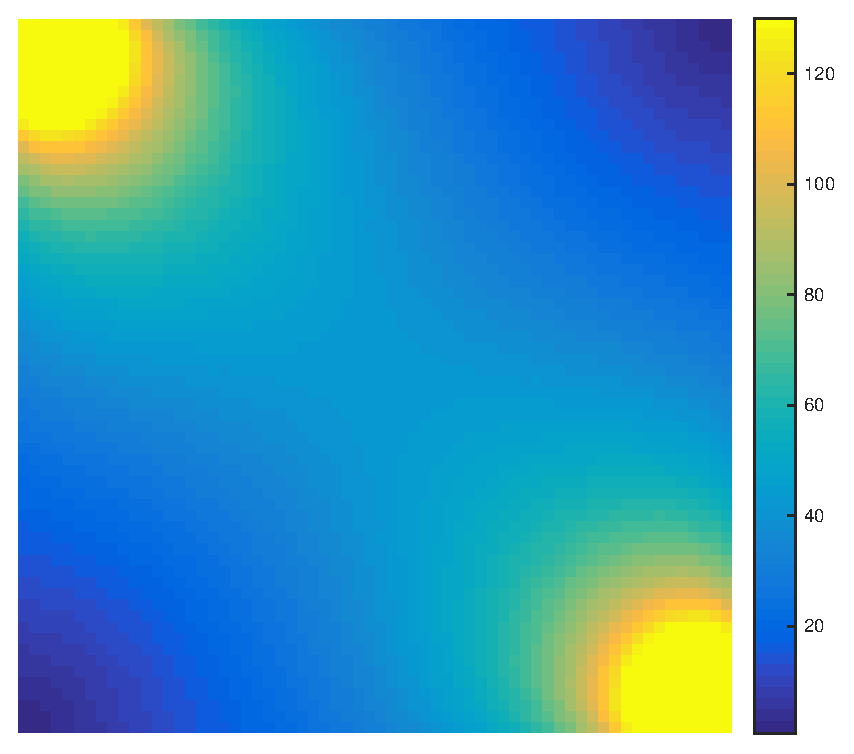
\includegraphics[width = .20\textwidth]{./figs/recTrue-PDE-1.eps} & 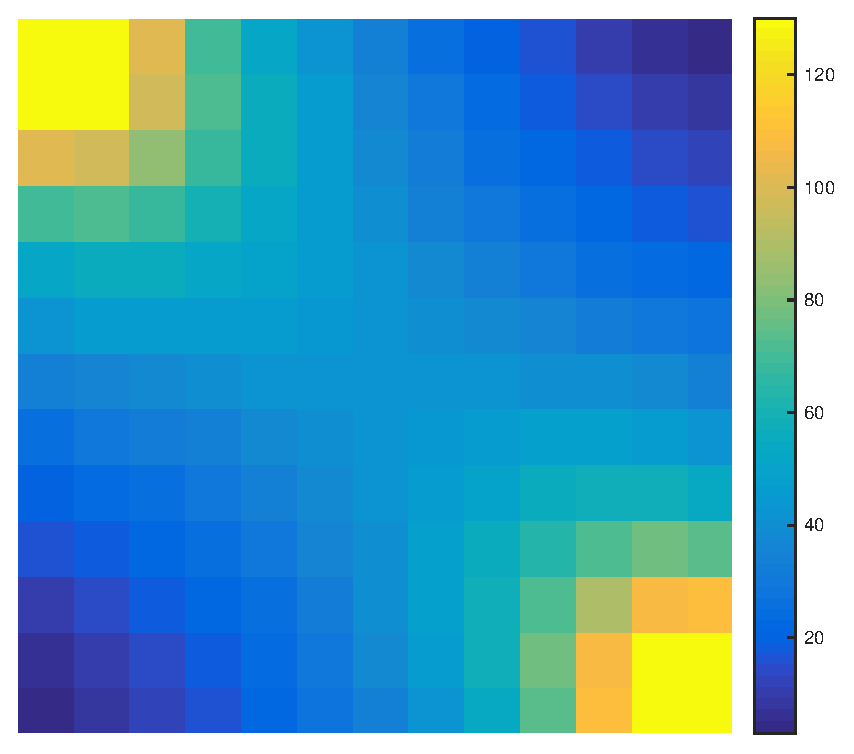
\includegraphics[width = .20\textwidth]{./figs/recTrue-PDE-5.eps} & 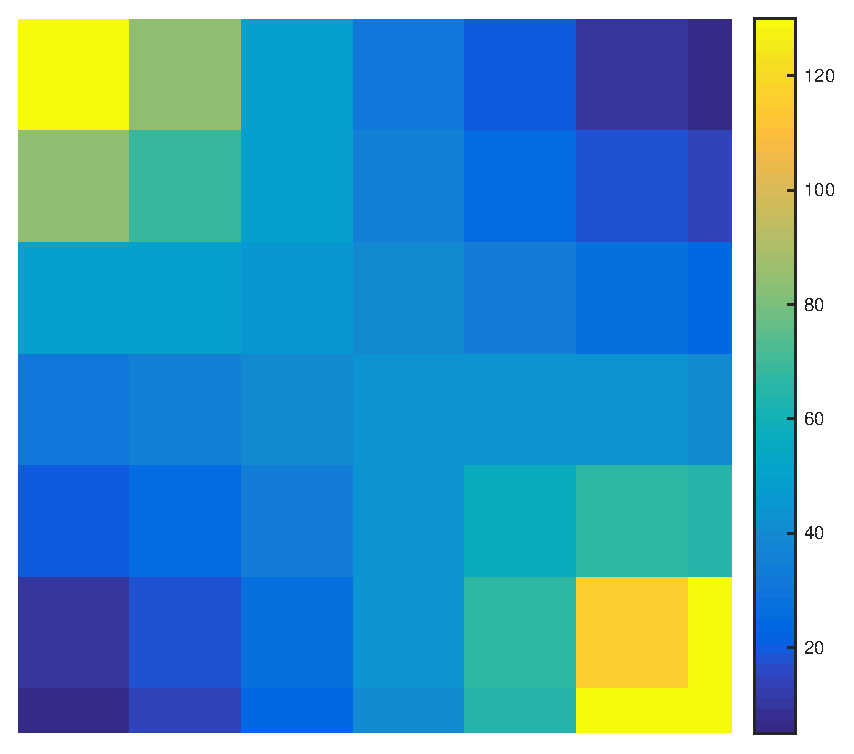
\includegraphics[width = .20\textwidth]{./figs/recTrue-PDE-10.eps}\\
			 \rbox{5ex}{bSVD} & 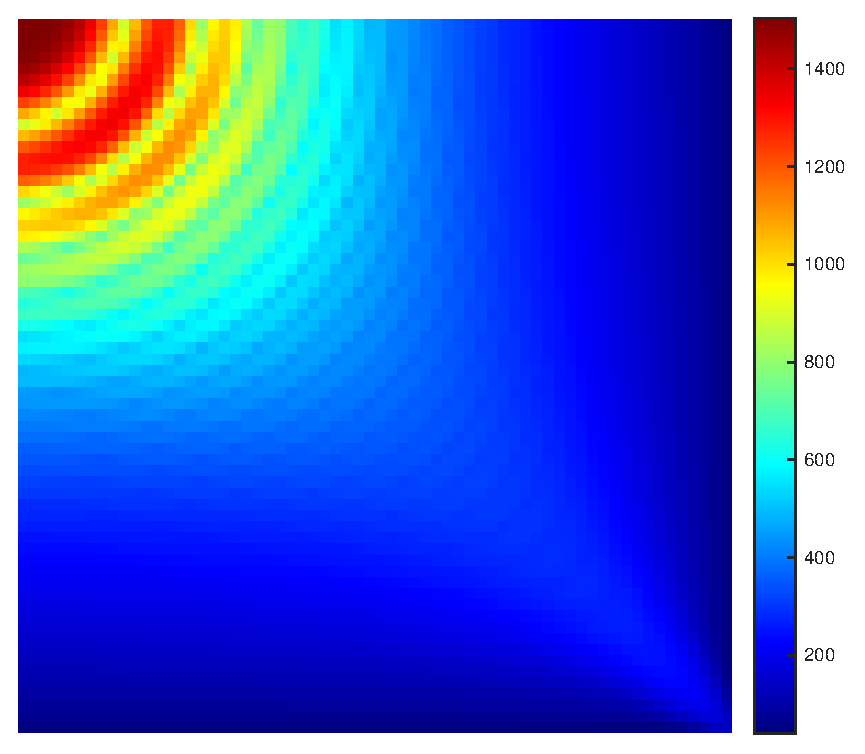
\includegraphics[width = .20\textwidth]{./figs/recCirc-PDE-1.eps} & 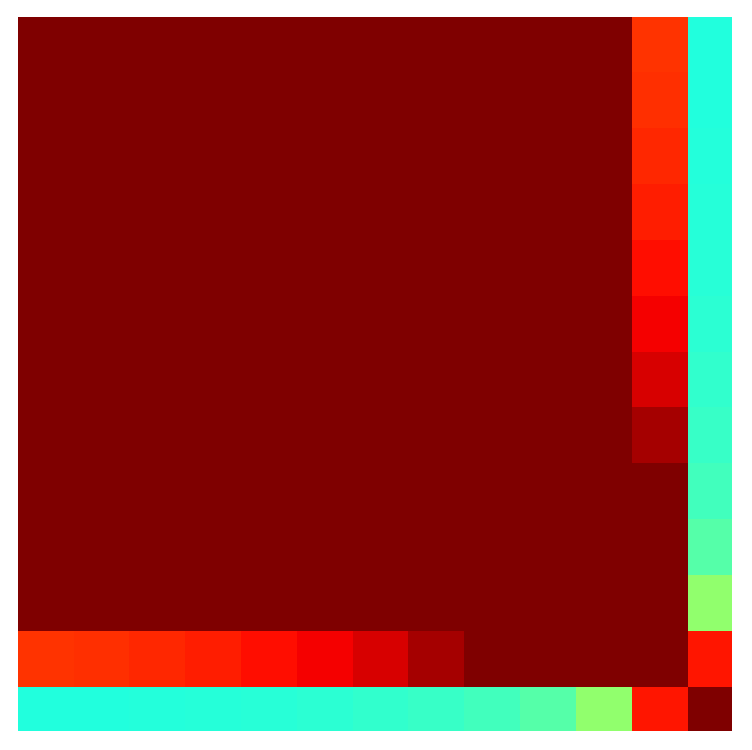
\includegraphics[width = .20\textwidth]{./figs/recCirc-PDE-5.eps} & 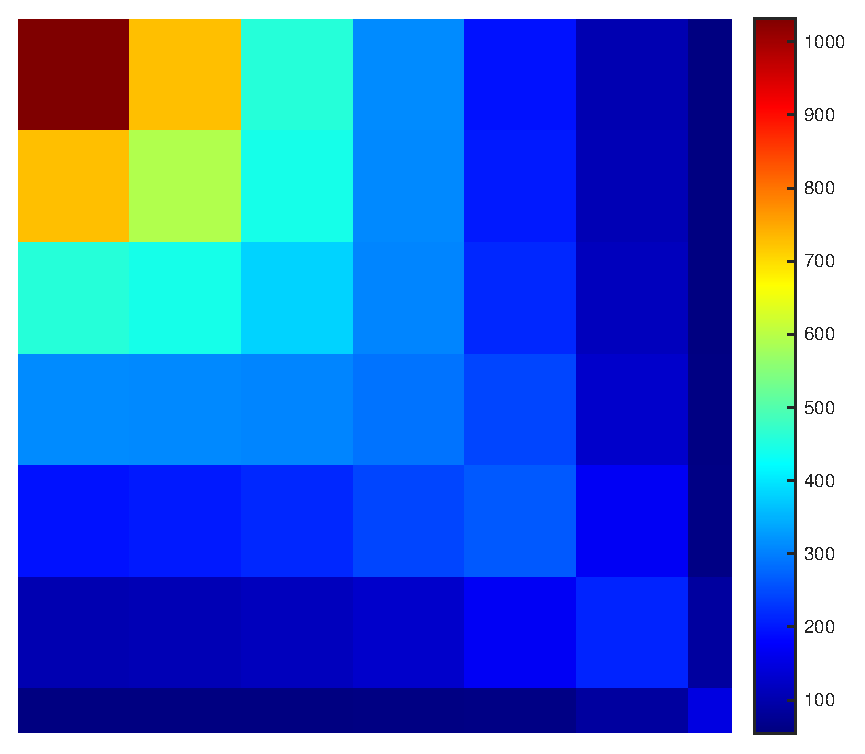
\includegraphics[width = .20\textwidth]{./figs/recCirc-PDE-10.eps}\\
			 \rbox{8ex}{MS} & 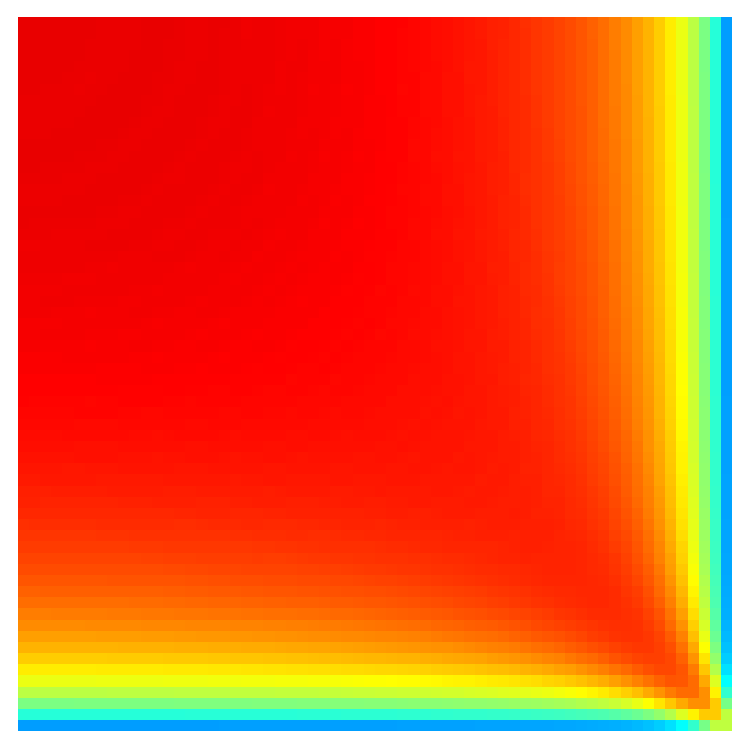
\includegraphics[width = .20\textwidth]{./figs/recMS-PDE-1.eps} & 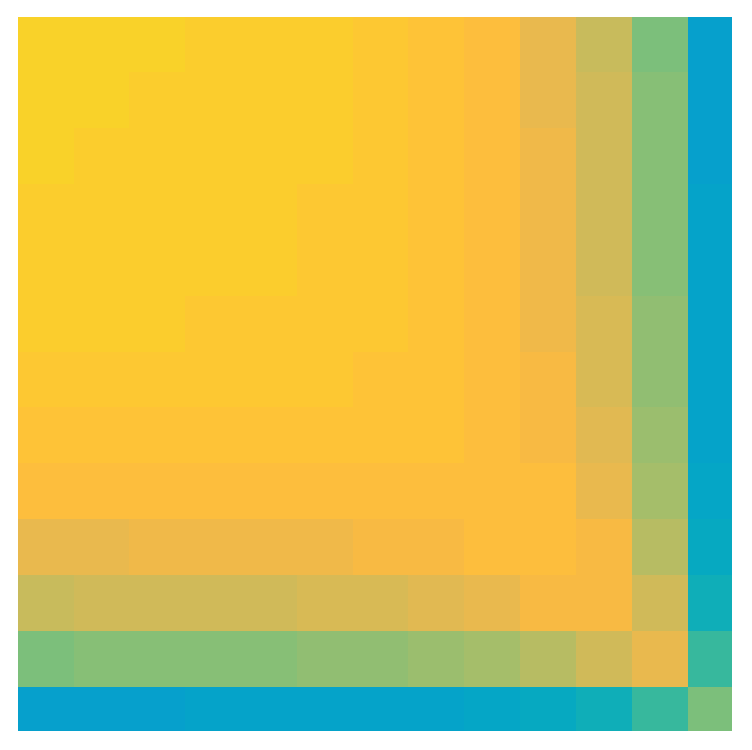
\includegraphics[width = .20\textwidth]{./figs/recMS-PDE-5.eps} & 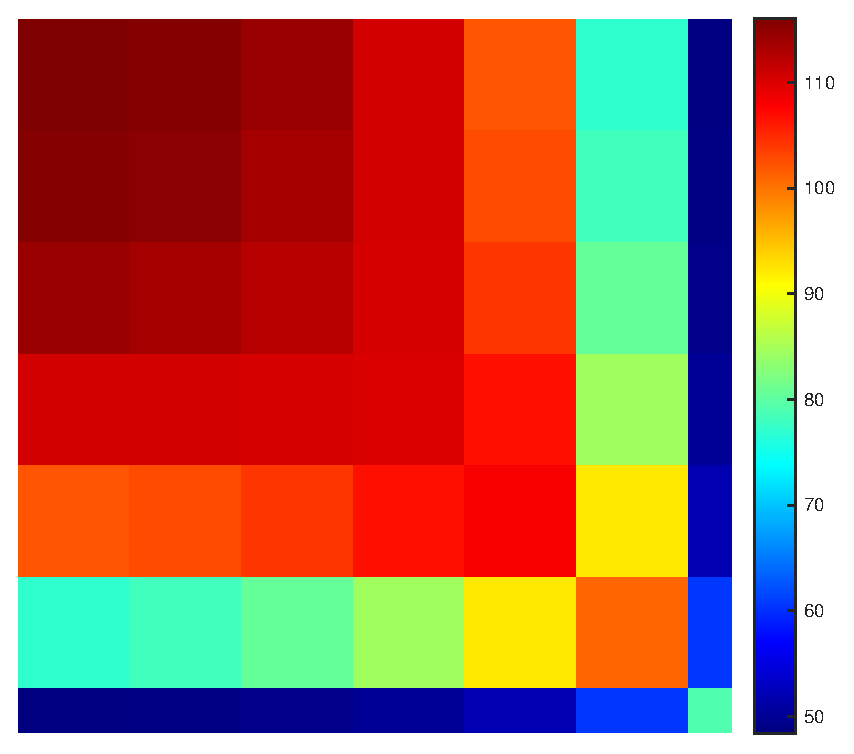
\includegraphics[width = .20\textwidth]{./figs/recMS-PDE-10.eps}\\			 			 			  
			   & (1,1) & (5,5) & (10,10)
		\end{tabular}
		\caption{Restoring the perfusion for different levels of discretization, displayed within the columns. Block size in voxels is shown in brackets. All results are given in [$\si{\siPml}$]. First Row: Ground-truth perfusion (cf. Section \ref{sec:flux2perf}). Second Row: Perfusion as estimated by bSVD. Third Row: Perfusion as estimated by the MS model. Both reconstruction methods fail in restoring the true perfusion, also reflected in the relative errors of Table \ref{tab:resultsSim}.}	
		\label{fig:resultsPMM}			
	\end{figure*}



	\begin{figure*}[]
		\centering
			\begin{tabular}{c c}
				 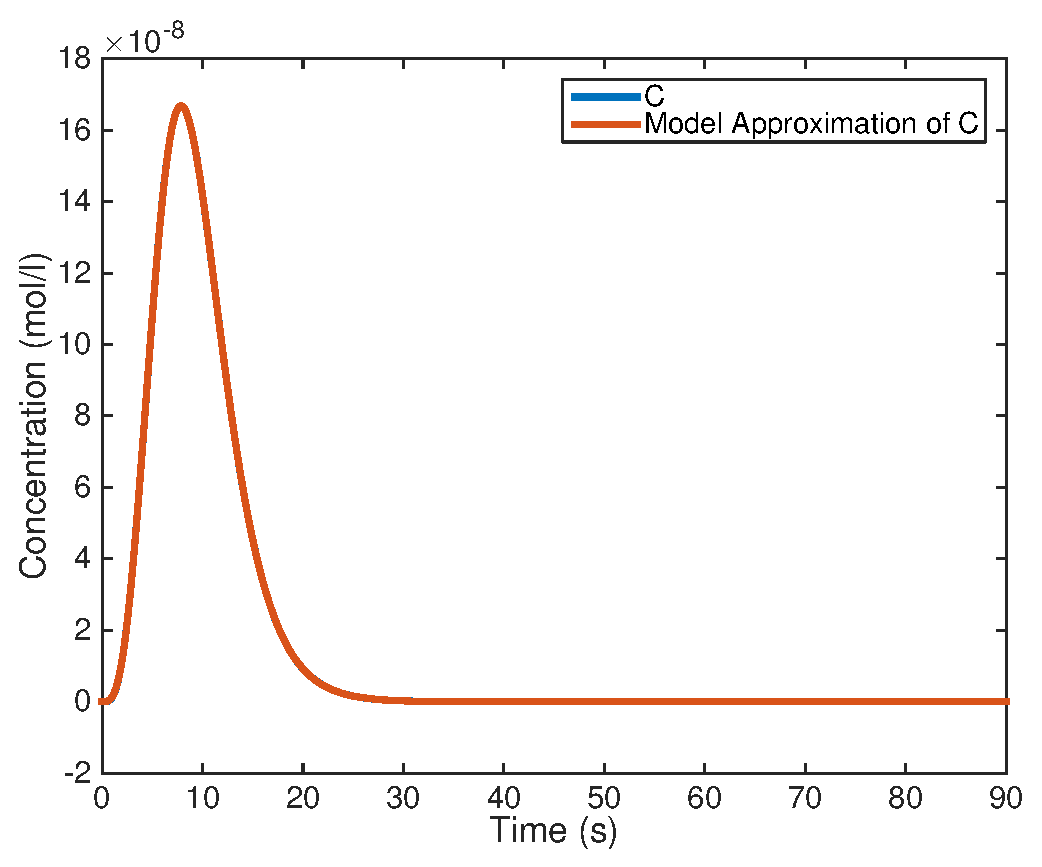
\includegraphics[width = .30\textwidth]{./figs/C-and-Crec.eps} & 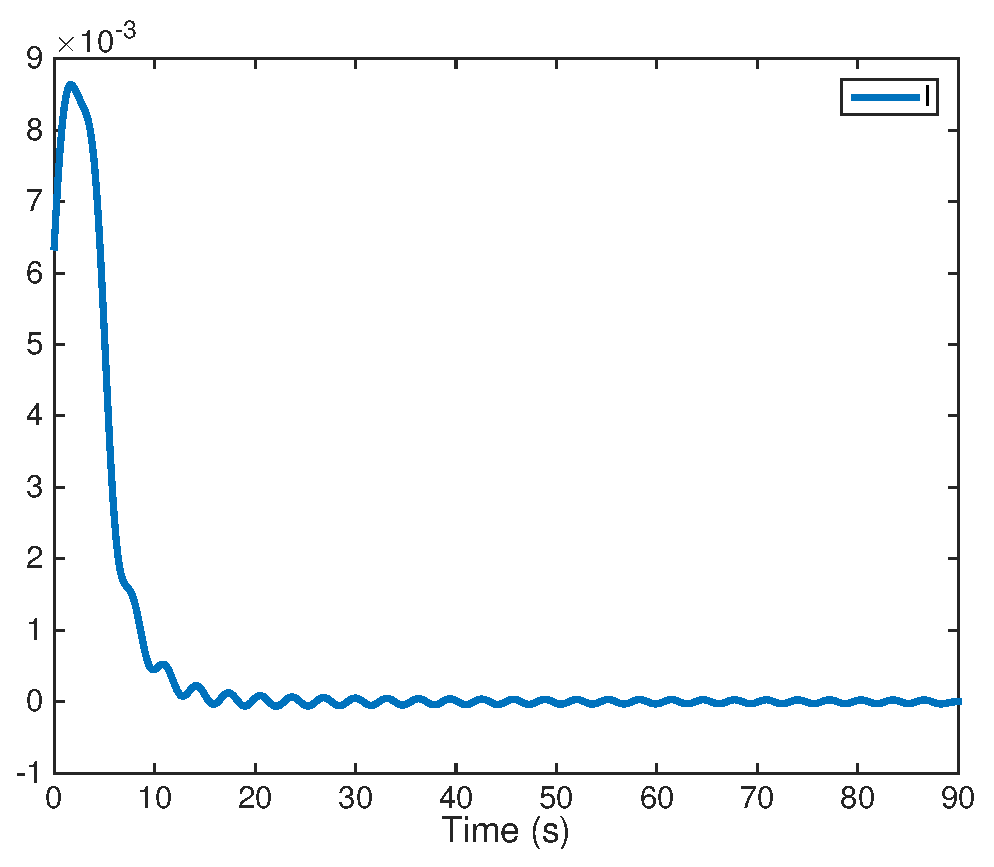
\includegraphics[width = .30\textwidth]{./figs/Irec.eps} \\
				 \multicolumn{2}{ c }{(a) Entire Domain, $C_T(x,t)$} \\
				 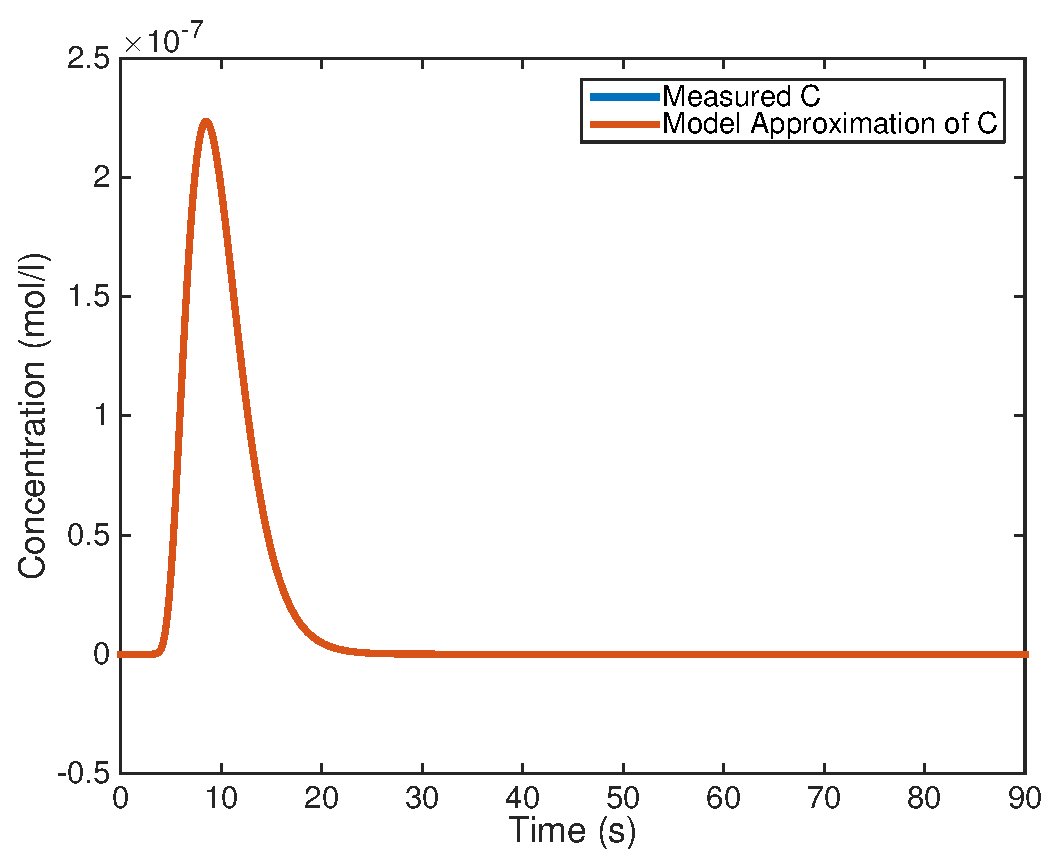
\includegraphics[width = .30\textwidth]{./figs/C-and-Crec-PDE.eps} & 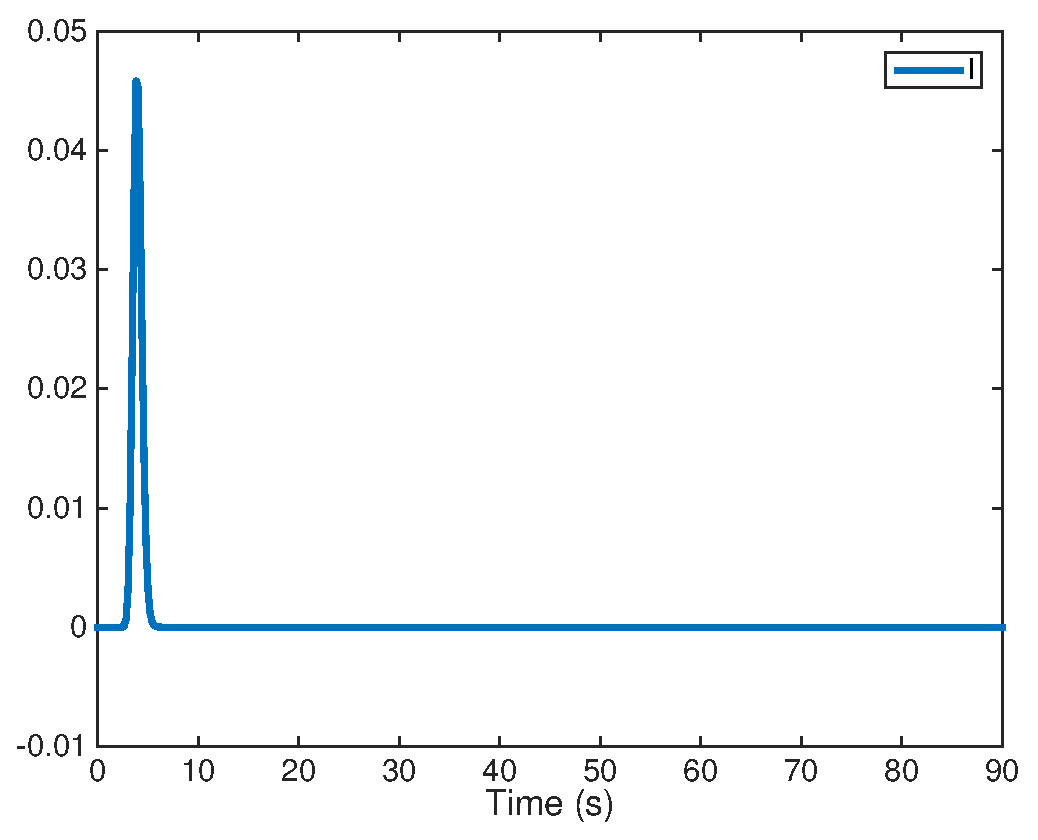
\includegraphics[width = .30\textwidth]{./figs/Irec-PDE.eps} \\			 
				 \multicolumn{2}{ c }{(b) Inside the capillary bed, $C_T(x,t)$ at $(i,j)=(50,50)$} \\				 
				 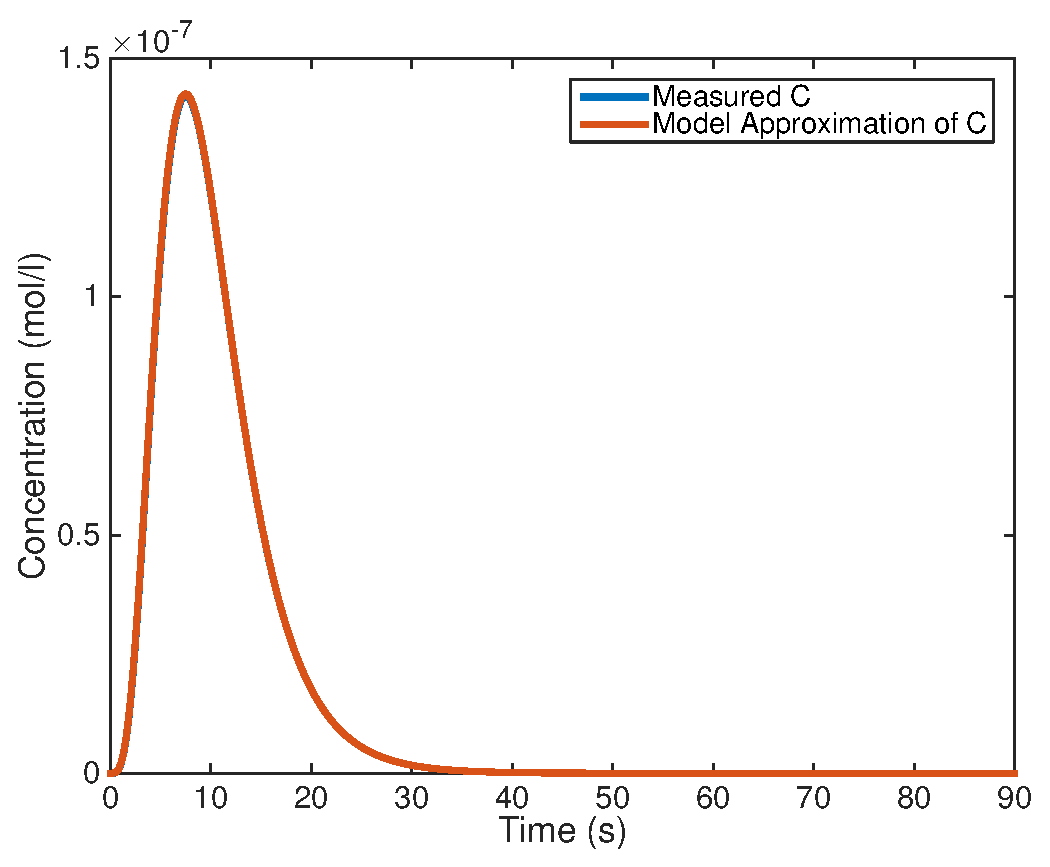
\includegraphics[width = .30\textwidth]{./figs/C-and-Crec-conv.eps} & 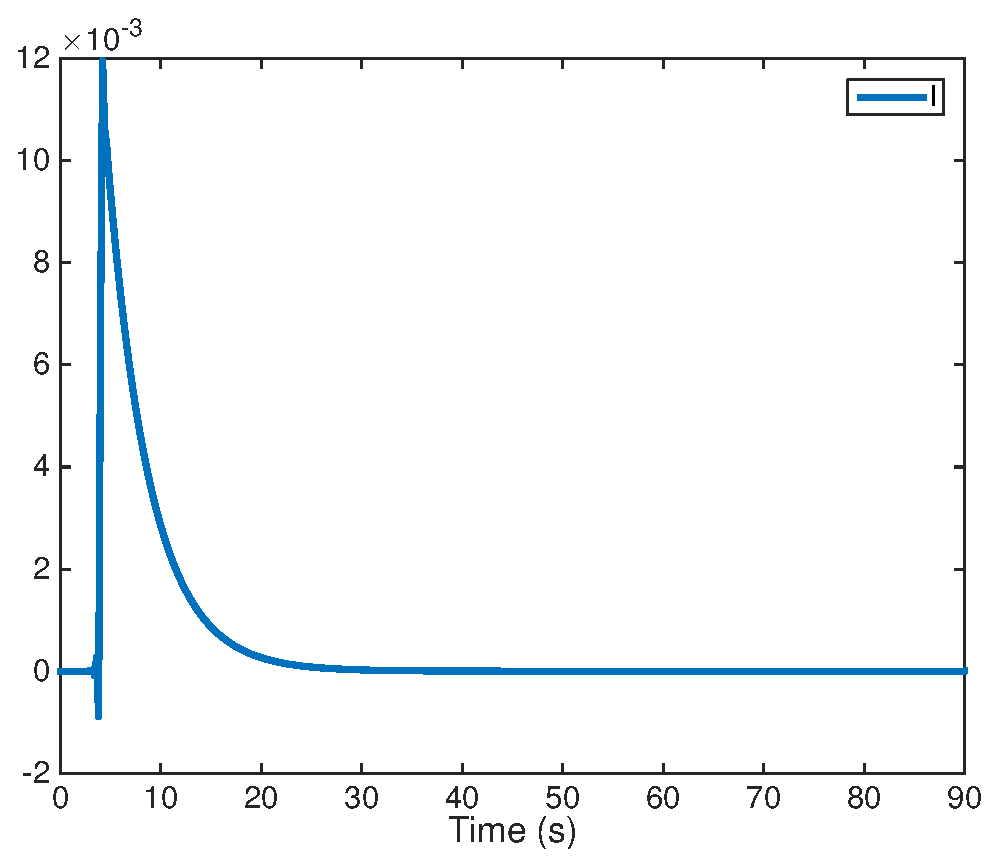
\includegraphics[width = .30\textwidth]{./figs/Irec-conv.eps} \\			 
				 \multicolumn{2}{ c }{(c) Inside the capillary bed, $C_C(x,t)$ at $(i,j)=(50,50)$} \\				 				 
			\end{tabular}
		\caption{Deconvolution by bSVD. First row: Results of bSVD applied to the map $C_T(x,t)$ generated with the transport equation \eqref{eq:conteq} using block-size (64,64) (i.e. entire domain). Second row: Results of bSVD applied to a single voxel of $C_T(x,t)$ in the inside of the domain. 56 row: Results of bSVD applied to a single voxel of the convolution data $C_C(x,t)$ in the inside of the domain. In all cases the model restored the measured concentration curves almost perfectly. Left to right: Reconstructed concentration $C(t)$ (left) and the impuls-response function $I(t)$ (right).}			
		\label{fig:deconvResults}
	\end{figure*}
	
	
	
	%--------------------------------------------------
	%--------------------------------------------------
	% Subsection: Results on Real Data
	%--------------------------------------------------
	%--------------------------------------------------	
	\subsection{Reconstruction of perfusion within real data}\label{sec:RealData}
 	Experimental results from Section \ref{sec:RecPhantom} indicate that application of the deconvolution model to patches of tissues violating the model assumptions would lead to overestimation of blood-flow as compared to the overall flow within the volume of interest.
	In order to validate this guess, we applied the deconvolution model to a clinically acquired human perfusion CT dataset of a 56 years old male male admitted to the University Hospital of Nijmegen with suspicion of stroke.
	The perfusion scan was obtained using a Toshiba Aquilon ONE scanner, pixel-size $\SI{0.43}{\milli\meter}\times\SI{0.43}{\milli\meter}$, slice thickness $\SI{0.5}{\milli\meter}$, contrast agent \SI{50}{\milli\liter} Xentix 300, total scan-time \SI{114}{\second}, time resolution ranging from \SI{2.1}{\second} in the early- to \SI{30}{\second} in the late phase of CA uptake.
	The arterial input function was manually selected by a medical expert within the middle cerebral artery.
	Since we expected to see local overestimation effects mainly for small voxel sizes, the data was processed at full resolution ($512\times512\times320$). 
	However, in order to deal with noise effects it was necessary to apply a prior gaussian smoothing with standard deviation of $1$ voxel.	
	Relative concentrations were estimated from the CT signal assuming a spatially independent proportionality constant.
	CBF was then estimated voxel-wise using the bSVD model, yielding an average CBF of \SI{64.357}{\siPml}.
	After that, we estimated the perfusion for the whole volume of interest by averaging the concentration values first and then performing the bSVD, yielding a total CBF of \SI{24.791}{\siPml}.
	Results are depicted in Fig. \ref{fig:RealData}
	
	
	
	\begin{figure*}[]\label{fig:RealData}
		\begin{tabular}{p{.3\textwidth} p{.3\textwidth} p{.3\textwidth} }
		 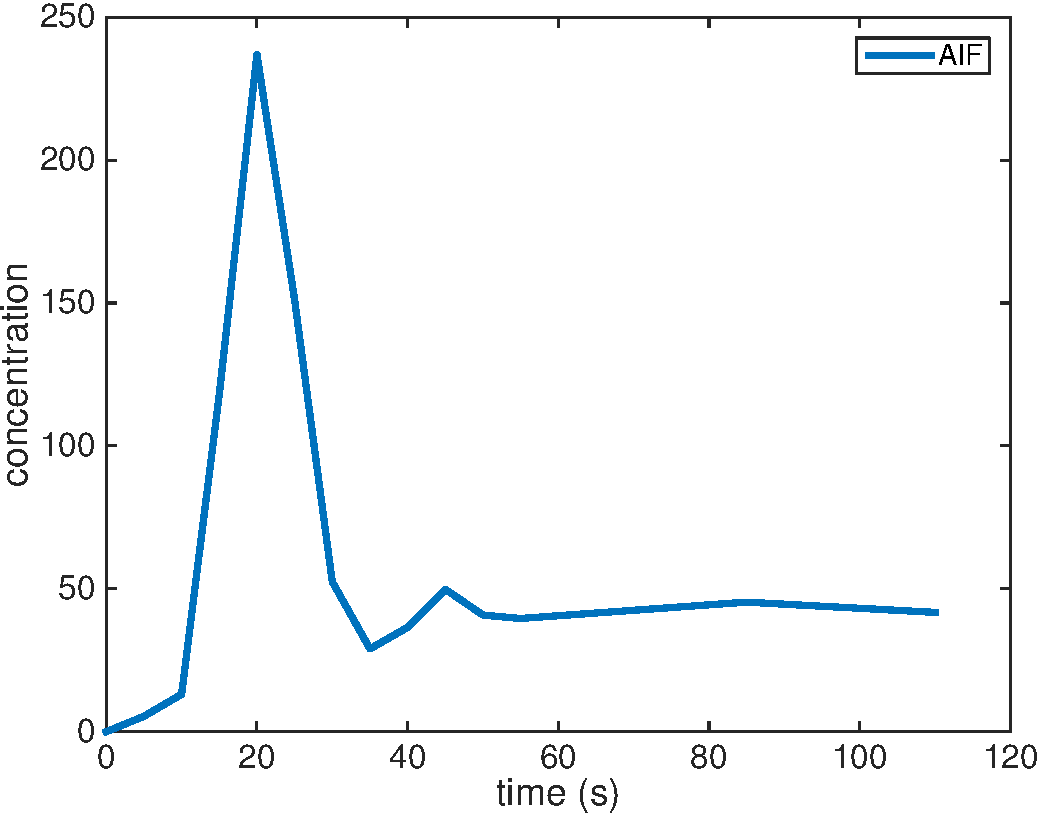
\includegraphics[width = .3\textwidth]{./figs/real_AIF.pdf} & 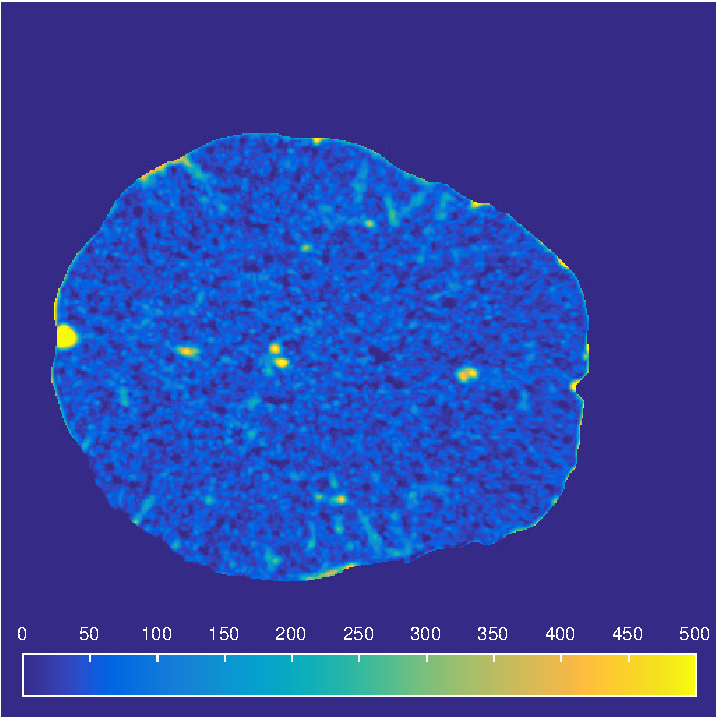
\includegraphics[width = .3\textwidth]{./figs/real_axial160.pdf} & 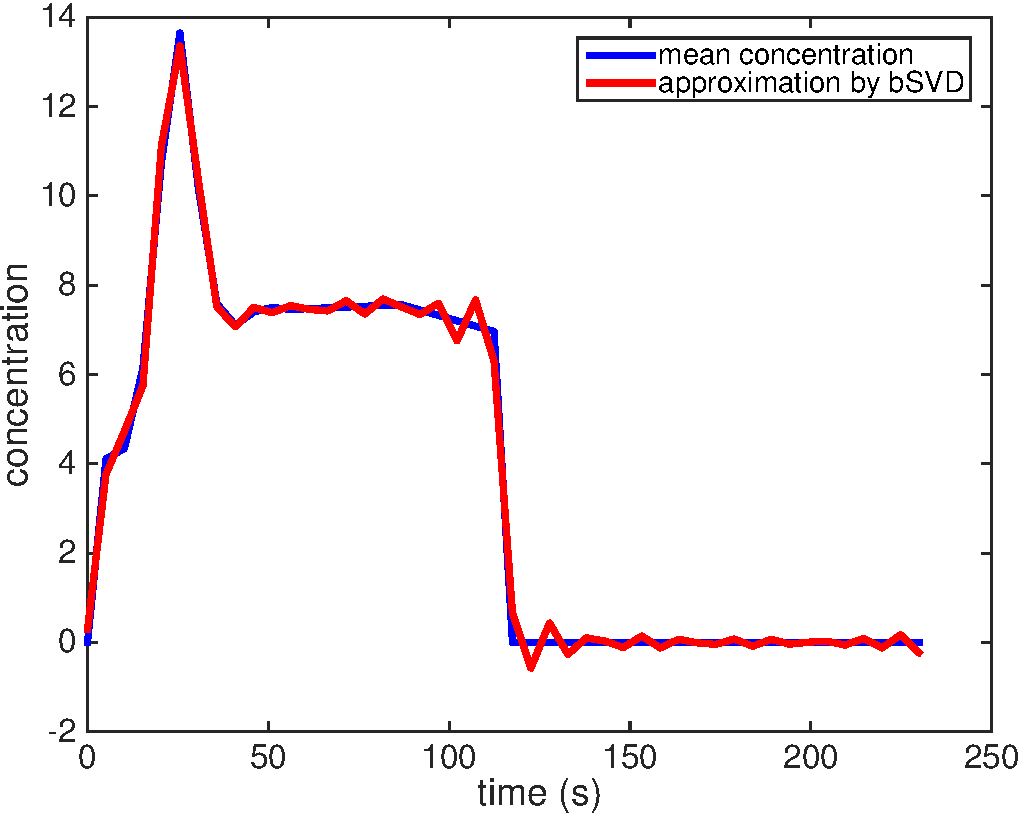
\includegraphics[width = .3\textwidth]{./figs/real_meanC.pdf} \\
		 (a) Arterial input function & (b) One slice of the voxel-wise CBF reconstruction.  & (c) mean concentration curve for the whole volume of interest and reconstruction.
		\end{tabular}
		\caption{Figure with results from the real-data experiments (see Sec. \ref{sec:RealData} for details on the data). The AIF shown in (a) was manually selected from the MCA. In (b) one slice of the voxel-wise CBF-reconstruction for a 3D volume of interest is shown. In (c) the mean-concentration curve for the complete 3D volume of interest and the approximation by bSVD is shown.}
	\end{figure*}
	

	
	
	%--------------------------------------------------
	%--------------------------------------------------
	% Section: Discussion
	%--------------------------------------------------
	%--------------------------------------------------	
	\section{Discussion}\label{sec:conclusion}
	
	Accurate measurements of CBV, CBF and MTT within the brain can provide crucial information used in clinical decision making. Originally, the traditional 1C models providing these parameters were developed for larger ROIs, and their validity for usage in field models has not properly been established. In this work we have developed a digital phantom for simulating blood flow within a slab of the capillary system. From the obtained flux field, we generate a perfusion map that was used to create two data sets of propagating concentration agent. The first data set was created as the solution of a linear transport equation, where every voxel acts as an arterial input to its neighbors. The other data set is based on a forward convolution model, where every voxel is exposed to the same arterial input function. This modeling setup with two distinct forward models has the property of isolating  possible errors caused by the numerical instability of the deconvolution methods.% The latter data set was mainly used to validate the , while the first data set was meant to represent a realistic data set as it can be obtained from a MR examination.
	
	Considering the data set created from the transport equation, $C_T(x,t)$, the results presented in Table \ref{tab:resultsSim} indicate low errors or $RE \leq 2.6 \%$ of both the MS and the bSVD model for restoration of the perfusion when applied to the entire domain. Using an arterial input function valid for the region as a whole is in agreement with physical assumptions required to derive the theory for traditional models. Thus, these results support the usage of traditional compartment models for whole organs with only one inlet and one outlet. 

However, the reconstruction of perfusion using MS and bSVD fails to a large extend with relative errors up to $859 \%$ for other block sizes that the entire domain, the error  apparently increasing for smaller block size. This observation of over-estimation indicates that traditional models for reconstructing perfusion are not valid for a situation where the global arterial input is not the correct arterial input for each of the smaller computational units. These results are also supported by the analytical analysis in Section \ref{sec:relating}, stating that in the continuous context traditional models are describing CA propagation for the Lagrangian setting, whereas traditional models are typically applied in an Eulerian setting. %\textcolor{red}{I'll think about this in more detail during the weekend.}
The observed over-estimation of perfusion is also predicted by the theoretical analysis in Section \ref{sec:flux2perf}, stating that the perfusion will be over-estimated with a factor proportional to the length of the streamlines. 
All these results are supported by the real-data experiments, where we showed local overestimation of perfusion for small voxel-sizes as compared to an averaging of concentrations for the whole volume of interest.
%Thus, in principle, one could apply the traditional methods, and scale the resulting perfusion map by the streamline length. 
%In such situation, assumptions of the traditional models are violated as the arterial input will be dispersed in unpredictable ways on the way from the inlet to the computational unit.

Considering the data set created from convolution, $C_C(x,t)$, from Table \ref{tab:resultsSim} it is clear that the bSVD model for deconvolution has a low error for voxel wise reconstruction. This result is closely related to the previously described "inverse-crime" where we used the same model for constructing the data as for reconstruction. However, in our case it provides evidence that the deconvolution algorithm used, the bSVD, is numerically stable, and that errors in true perfusion are unlikely to arise from numerical instabilities of the deconvolution. This conclusion is also supported by Fig. \ref{fig:deconvResults}, where the measured and the restored concentration curves are more or less identical for various block sizes and various input data. However, despite the success of restoring the concentration curves, the usage of a model in an "inverse-crime" settings can not be used to support the physical validity of the model, but only the numerical stability of the deconvolution in this case. 

Interestingly, the MS model fails in restoring the perfusion for all block sizes of the forward convolution data. The reason for this is probably that within the MS model there is an assumption of no output of CA as the arterial input peaks. This assumption is clearly violated as the forward convolution model assumes an instantaneous transport of CA both into as well as out of the domain due to the assumption of well-mixed compartments.
	 
Regarding the CBV estimates, one can observe from Table \ref{tab:resultsSimphi} that both data sets $C_T(x,t)$ and $C_C(x,t)$ could successfully be used to restore the CBV. Various block sizes also had little impact on the results. These results are in well agreement with the analytical proof of CBV in Section \ref{sec:CBV}, stating that equation \eqref{eq:CBV} is valid for entire organs as well as for single voxels. Thus, these results support the usage of \eqref{eq:CBV} for computing the CBV with high accuracy for any type of block size, including single voxels.
	 
	 
In light of our current findings we want to focus on the usage of traditional compartment models for voxel wise perfusion in the brain. Our results indicate the traditional models should only be used for larger computational units where the arterial input is an actual arterial input for the domain as a whole. The development of new field models for perfusion is therefore highly demanded, in line with approaches described in \cite{sourbron14}. 

With these conclusions in mind, our results are only valid for one-compartment systems like the brain with an intact blood-brain-barrier. For other organs or pathological situations with a leakage of tracer into the extravascular space, the observed effects described in this work are yet to be discovered.
	 
Apparently, the true perfusion in a brain is unknown, and a gold standard is therefore not accessible for real data on a voxel wise basis. As an alternative, we propose to use simulated data sets like ours for benchmarking of new perfusion reconstruction algorithms. Applying various reconstruction methods  to the same data set with a known ground truth would make it easier to compare and evaluate the performance. 
	 
	 
%	We have in this work presented a porous media model for simulating flow in porous tissue. 
%	Results in Tab. \ref{tab:resultsSim} are indicating good performance of both models to restore the perfusion for an entire volume. 
%	Errors are $2.6\%$ for the Maximum-Slope model and $1.3\%$ for the deconvolution model.
%	However, the results of the deconvolution model depend on a heuristic choice of the regularization parameter \missingsource.
%	Results on a voxel-level are looking quite different (see Tab. \ref{tab:resultsSim}).
%	Here the perfusion is grossly overestimated by both the deconvolution model and the the maximum-slope model.
%	Errors are in the range of far over $100\%$, indicating a lack of validity of the classic models.
%	This impression is supported by the recovered impuls-response functions, displayed in Fig. \ref{fig:deconvResults}.
%	Although classic models assume monotonously decreasing residue-functions, the impuls-response functions we obtained are clearly violating this property.
%	These effects might be due to dispersion effects \cite{calamante03} and are subject to current investigations.
%	
%	However, as expected the deconvolution model worked quite good for the ConvM-dataset (see Tab. \ref{tab:resultsSim}). 
%	But results are deteriorating if several volumes are averaged, leading to errors of up to $20\%$.
%	This can be interpreted that even if the assumptions of the traditional models are fulfilled, parameter-estimation will be sensitive with respect to broad resolutions.
%	As already described in Sec. \ref{sec:NumExp}, the maximum-slope model fails to restore perfusion correctly due to the assumption of well-mixed compartments.
%	Taking into account all of these observations we arrive at the following conclusions:
%	If traditional models are valid, a too broad spatial resolution might lead to significant errors in the estimation of perfusion parameters.
%	On the other hand, a too fine resolution might lead to voxels placed inside of the capillary bed and hence to a dramatic overestimation of CBF.
%	A method to determine the appropriate size of voxels is unknown to the authors, as it is coupled to the validity of the assumptions on the models.
	
	Concluding, we have proposed a novel method to validate traditional models for perfusion analysis. We have shown that within the assumption of a common AIF, valid for the entire domain, traditional models for restoring the perfusion are reliable. However, when sub-dividing the computational units into smaller ROIs, even down to voxels, significant errors are introduced. Furthermore, these errors are not likely to be related to the deconvolution method, but are rather related to violation of the physical model assumptions, and the computed perfusion will be over- or under-estimated with a factor proportional to the streamline length. 
	%Still, voxel wise perfusion estimates are extensively reported in the literature \cite{Warwick2008, Arkink2012,White2012,Feng2013,Chen2011}, even though the validity of used methods has not been established. 
	The field models described in this paper are not suited for inverse modelling like perfusion estimation from real imaging data. Nevertheless they will fill the role as a framework for generation of synthetic benchmarks.  In light of these results, future work should focus on the development of field models for perfusion measurements, taking into account the local constellation and neighbourship of voxels. % By these means one could develop reliable models also for voxel wise estimates.   % In this process it is useful to have benchmarking models for judging reliability of the models. We suggest that our simulated flow model could be used for such comparisons.
	 
%	Based on porous media modeling, we described an easily extendable model to simulate CA-flow through a volume of interest.
%	The proposed model assumes stationary and linearity of flow as well as spatially constant blood-volume.
%	In this form it is completely in line with current pharmacokinetic modeling \cite{sourbron14}.
%	In order to connect (medical) volume perfusion with (physical) surface flow, a novel relationship between these two was introduced.
%	For the experiments we have confined to a most simple setup, modeling a volume of interest with one inlet, one outlet and constant porosity.
%	However, a more sophisticated simulation including more inlets and outlets at spatially varying locations as well as porosity can be set up readily.
%	We showed that under these assumptions traditional models are yielding good results for perfusion values and can indeed be used with high reliability.
%	But as soon as the assumptions are violated, which is the case for the capillary bed, significant errors are introduced.
%	Since current validation of deconvolution algorithms is typically performed in the inverse-crime setting, the developed model could be used as an additional reference standard for validation.
%	In the proposed modeling, exact perfusion values for the whole tissue can be modeled. 
%	Using this method it is hence possible to quantify errors introduced by e.g. different numbers of input and output, more complex flow or even leakage.
%	
%	As future work we will further investigate the impuls-response functions of the capillary bed and will simulate more complex phenomena in the tissue.

	
	%--------------------------------------------------
	% Bibliography
	%--------------------------------------------------
	\bibliographystyle{IEEEtran}	
	\bibliography{./bibliography}

	\appendix
	

	
	\section{Numerical Implementations of the Synthetic Model for Capillary Perfusion}
	\label{sec:numsynt}
	
	In this section we describe how the models were implemented numerically.
	For simplicity the domain is discretized by a regular cartesian grid of size $m \times m$ with a regular cell-spacing $h$.
	The proposed method may be extended for non-regular grids in an analogous fashion.	
	
	%----------------------------------------------------------
	% Subsection: Discretization of the singe phase flow model
	%----------------------------------------------------------
	\subsection{Discretization of the Single Phase Flow Model using TPFA} \label{sec:numflow}

	Equation \eqref{eq:flowmodel} was solved using the TPFA method widely used in reservoir mechanics \cite{Aarnes2007}.
	Integrating \eqref{eq:flowmodel} across a small domain (voxel) $\Omega_i \subset \Omega$ and applying the divergence theorem yields
	\begin{equation}
		\int_{\partial \Omega_i}   -(\lambda \nabla p) \cdot n \diffint s = \int_{\Omega_i}Q \diffint x
	\label{eq:TPFAint}
	\end{equation}
	with conductivities $\lambda := k/\mu$.
	Defining $\partial \Omega_{ij}$ as the boundary between neighboring voxels $\Omega_i$ and $\Omega_j$, only the flux component perpendicular to $\partial \Omega_{ij}$ will drive the flow between these voxels.
	The component of $\nabla p$ pointing along the normal vector of $\partial \Omega_{ij}$ can in terms of cell centered pressure values $p_i$ and $p_j$ be replaced by
 	$\Delta p_{ij} := (p_j - p_i)/h$.
	Hence, the total flux across the face $\Gamma_{ij}$ can be approximated by
	\begin{equation}
		\Delta p_{ij} \int_{\partial \Omega_{ij}}\lambda \diffint s \approx (p_i - p_j) \underbrace{\frac{\lambda_{ij} \vert \partial \Omega_{ij} \vert}{h}}_{:=t_{ij}}.
		\label{eq:pressnum}
	\end{equation}
	Here, $\lambda_{ij}$ denotes an approximation of the mean conductivity on $\partial \Omega_{ij}$, where $\lambda_{ij}$ is computed by harmonic averaging from the requirement of continuity in $p$ on the midline of $\partial \Omega_{ij}$.
	The terms in \eqref{eq:pressnum} not depending on the pressure $p$ are collected into the transmissibilities $t_{ij}:=|\partial \Omega_{ij}|\lambda_{ij}/h$.
	Approximating the right hand side of \eqref{eq:TPFAint} as $\int_{\Omega_i}Q \diffint x \approx Q_i |\Omega_{ij}|$ yields a linear system which can be solved for the pressure $p$. Due to the Fredholm alternative, we imposed Dirichlet boundary conditions for one voxel within $\Omega$ to ensure uniqueness.
	Note that $p,k,Q$ and $\mu$ are defined cell-centered whereas the resulting flux $q$ is discretized on a staggered grid, corresponding to the voxel faces.


	%----------------------------------------------------------
	% Subsection: Discretization of the transport equation
	%----------------------------------------------------------
	\subsection{Discretization of the Transport Equation} \label{sec:numtrans}
	The transport described in \eqref{eq:conteq} was implemented using first order upwinding \cite{Patankar80}.
	Let $c_{ij}$ be a cell centered voxel tracer concentration with respect to the fluid volume on the cell face $\partial \Omega_{ij}$ adjacent to voxel $i$ and voxel $j$, and let $n_{ij}$ be the outer normal vector of $\partial \Omega_{ij}$. Also, the cell staggered fluid flux is represented as a vector $q_{ij}$.
	The total CA-flux over the face $\partial \Omega_{ij}$ for any time point was approximated by
	\begin{equation}
	\int_{\partial \Omega_{ij}} c_{ij} (q_{ij}\cdot n_{ij}) \diffint s \approx
	\begin{cases}
	c_i q_{ij,n} \vert \partial \Omega_{ij} \vert & \text{if } q_{ij,n} \geq 0,\\
	c_j q_{ij,n} \vert \partial \Omega_{ij} \vert & \text{if } q_{ij,n} < 0,
	\end{cases}
	\end{equation}
	where $q_{ij,n} = q_{ij} \cdot n_{ij}$ is the normal component of the flux across $\partial \Omega_{ij}$.
	Keeping track of in- and outflow for each voxel yields an explicit discretization scheme to set up the transport simulation. We used a time step of $\Delta t = 0.002 s$ in a forward Euler time stepping of \eqref{eq:conteq}.
	A conversion of $c_i$ into $C_i$ was performed via the relation $C_i = c_i\phi_i$. The overall concentration map $C_i$ was later used for the inverse problem of restoring CBV and CBF.
	
	

\end{document}